%%%% Le fichier lecture.cls n'est pas le fichier original fourni par l'auteur. Changement au niveau du package geometry pour la gestion du oneside
% Teexuds
\documentclass[french,course,oneside,theoremnosection]{lecture}
\usepackage[T1]{fontenc}
\usepackage{lipsum} % Only needed to generate dummy text for sample.tex
\usepackage[french]{babel}
\usepackage{enumerate,hyperref,algorithm,algpseudocode}
\usepackage{comment}

% !!!!! The comment package is used to comment out a LARGE portion of text

%% Defining backmatter to get the reference after the figure in appendice
\makeatletter

\newcommand\frontmatter{%
    \cleardoublepage
  %\@mainmatterfalse
  \pagenumbering{roman}}

\newcommand\mainmatter{%
    \cleardoublepage
 % \@mainmattertrue
  \pagenumbering{arabic}}

\newcommand\backmatter{%
  \if@openright
    \cleardoublepage
  \else
    \clearpage
  \fi
 % \@mainmatterfalse
   }

\makeatother
%%%


%%%% Further box
\usepackage{tcolorbox}
\tcbuselibrary{breakable}
\newenvironment{further}[1]
{\begin{tcolorbox}[colframe=gray!50, colback=gray!5, arc=0pt, outer arc=0pt, boxrule=0.5pt, title=#1, breakable]}
{\end{tcolorbox}}
\usetikzlibrary{matrix}
 %\usetikzlibrary{calc}
%%%






%\usepackage{mparhack}

%%%On règle le problème des notes de marges qui changent de côté même en oneside
\makeatletter
%\reversemarginpar
\@mparswitchfalse%
\makeatother

%%%% Largeur des notes de marges
\setlength\marginparwidth{0.9in}


%
% First, provide some data about this document
\title{Structures mathématiques}
%\subtitle{Mathématique élémentaire}
%\shorttitle{Math. élem.} % For headers; if undefined, the usual title will be used
\ccode{BMATH} % Most of these data are not compulsory
%\subject{Opérations élémentaires, fractions, arithmétique, logique élémentaire, notion de fonction}
\author{Bruno Teheux}
%\spemail{euler@email.com}
\email{bruno.teheux@uni.lu}
%\speaker{Speaker's name}
%\date{14}{00}{2020}
%\dateend{20}{12}{2020}
%\conference{Lecture hall 7}
\place{Université du Luxembourg}
%\flag{An extra line if you need it.}
\attn{Ces notes de cours sont destinées aux étudiant·e·s du premier semestre du Bachelor en mathématiques de l'Université du Luxembourg pour l'année 2023~-~2024. Elles sont complétées par une liste d'exercices dont la résolution fait partie intégrale de la formation.

\medskip

\rule{0.12\textwidth}{0.3pt}
\medskip

Version du \today

\smallskip

\textcolor{red}{Nous tâchons de corriger les erreurs typographiques régulièrement. Les mises à jour seront déposées en ligne, dans le dossier partagé.}

%\medskip
%
%Laissez le hasard venir à moi.
%\medskip
%
%Le Schmilblick est un objet rigoureusement intégral qui ne sert absolument à rien et peut donc servir à tout\ldots~ (Pierre Dac)
}

%\morelink{Nothing}
%
% And then begin your document
\newcommand{\R}{\mathbb{R}}
\newcommand{\N}{\mathbb{N}}
\newcommand{\Z}{\mathbb{Z}}
\newcommand{\Q}{\mathbb{Q}}
\newcommand{\struc}[1]{\langle #1\rangle}
\newcommand{\co}{\mathrm{co}}
\newcommand{\Cl}{\mathrm{Cl}}
\newcommand{\pr}{\mathrm{pr}}
\newcommand{\iimplies}{\Rightarrow}
\newcommand{\ifff}{\Leftrightarrow}
\newcommand{\dom}{\mathrm{dom}}
\newcommand{\im}{\mathrm{im}}
\newcommand{\inco}{\parallel}
\newcommand{\supp}{\mathrm{supp}}
\newcommand{\ppcm}{\mathrm{ppcm}}
\newcommand{\alg}[1]{\mathbf{#1}}


\hyphenation{ma-th\'ema-tique ma-th\'ema-tiques}


\begin{document}
%;;; Principe de substitution;;;
%
%;;;Logique, langage naturel et AI;;;
%
%;;;Metalangue;;;
%
%;;;Voir avec Ann pour les problèmes de français?;;;
%
%;;;Variable muette;;;
%
%;;;Mot définit en italique;;;
%
%;;;Montrer comme synonyme de prouver;;;
%
%;;;Exercice montrer que le produit cartésien est produit au sens catégorie;;;
%
%;;; Sess wikipedia for exercices on Cartesian product;;;
%
%;;;Union, intersection d'une famille d'ensembles (pas nécessairement finie)? Union et intersection du vide?;;;
%
%;;;La restriction d'une fontion injective est injective;;;
%
%;;;Definir l'union de fonctions;;;
%
%;;;Definir nombre decimal;;;
%
%;;;Exercices sur les familles de sous-ensembles;;;
%
%;;;Faire une liste des termes qui évoque une implication et ceux qui évoquent une équivalence';;;
%
%;;;L'union de bijections disjointes est une bijection disjointe;;;
%
%;;;Avec WOP: Tout entier naturel $n>1$ qui n'est pas premier est divisible par un nombre premier;;;
%
%;;;différence entre équation et identité;;;
%
%;;;vous renonce à des privilèges que vous n'avez pas, donc vous ne renoncer à rien;;;
%
%;;;combinaison et triangle de pascal?;;;

\section{Introduction}
Le cours de structures mathématiques a deux objectifs. Le premier est d'introduire petit à petit un certains nombres d'objets mathématiques \og~structurés~\fg{} dont la présence est omniprésente dans le développement des ma\-thé\-ma\-tiques con\-tem\-poraines. Ces structures, vous les utiliserez quotidiennement dans votre vie étudiante, souvent sans vous en rendre compte, ou quand vous serez devenus mathématicien·nes.

Le deuxième objectif est de vous initier à la \emph{structure de la pensée mathématique}. L'objet d'étude des mathématiques est constitué d'idées. Mais contrairement aux autres disciplines qui ont des idées comme champs d'investigation (comme la philosophie, la métaphysique, l'économie\ldots) les idées mathématiques ont la remarquable propriété d'être universelles: une fois validées, elles les sont pour tous, partout et pour toujours. N'est-il pas remarquable que nous utilisons toujours des théorèmes prouvés par Euclide ou Archimède plusieurs siècles avant note ère?

Cette universalité n'est pas arrivée par hasard. Elle est le produit de la rigueur de la pensée mathématique. Pourquoi  les mathématicien·nes sont iels reconnu·es pour leur rigueur? En voici la raison:  pour que tout le monde s'accorde sur une idée, celle-ci doit être précisément énoncée. Formellement, cela passe par l'utilisation d'un (ou plutôt plusieurs) langage mathématique, avec une grammaire précise qui délimite le pouvoir d'expression de ce langage.  

Heureusement, de nombreuses libertés peuvent être prises par rapport à ce langage pour \emph{communiquer} les mathématiques. Pour jouir de ces libertés, il faut en connaître les limites. C'est une apprentissage indispensable durant la première année d'étude en mathématiques. Elle se fait au travers de tous les cours du programme~-~souvent de manière vicariante (\emph{i.e.}, par observation du comportement des professeur·e·s et assistant·e·~s). Dans ce cours, nous nous attacherons particulièrement à la formalisation (ou plutôt la \emph{formulation}, au sens de la mise en mots) de cet apprentissage. Bref, nous espérons que ce cours aura un effet \emph{structurant} sur votre pensée mathématique! 

\subsection{Transition lycée~-université}

Vous êtes étudiant·e à l'université! Que signifie ce nouveau statut? On peut le résumer de la manière suivante: \emph{vous êtes totalement responsable de votre apprentissage}. Dans ce cadre, le rôle de vos enseignant·e·s et encadrant·e·s est de vous fournir différents outils pour apprendre (cours en présentiel, notes de cours, bibliographie, listes d'exercices, Math Forge\ldots) À vous de sélectionner et d'utiliser ceux qui vous conviennent le mieux.

Du point de vue de la quantité de travail, on peut grossièrement estimer que  \emph{quelque soit la quantité de travail que vous déployiez au lycée, elle sera double à l'université}. Ne vous laissez pas dépasser par la quantité de matière!

Du point de vue du contenu mathématique, vous allez découvrir un nouvel univers. Petit à petit, les exercices qui vous seront proposés seront de moins en moins routiniers et demanderont de plus en plus de créativité mathématiques.

Mais ne paniquez pas! Tout est mis en place pour adoucir cette transition et tou·te·s les étudiants qui ont été diplômés sont passés par là avant vous!


\subsection{Comment lire ces notes?}
Ces notes servent de référence pour le cours de Structure Mathématiques. Elles font foi\footnote{Il s'agit de la première édition, et elles contiennent sans doute encore de nombreuses erreurs et fautes de frappe.} en ce qui concerne les définitions, énoncés de théorèmes\ldots~Elles doivent être consultées régulièrement, après chaque cours. Elles sont écrites dans une optique d'apprentissage: elles ne sont pas succinctes (surtout au début) afin de mettre en évidence les pièges connus dans les premiers pas d'un apprenti mathématicien·ne. Parfois, elles ouvrent des perspectives sur la matière couverte.

Elles constituent un complément à la participation au cours théorique, auquel elles ne pourraient se substituer, et servent de base à la participation \emph{active} aux séances d’exercices.

\subsection{Théorème, lemme, conjecture...}
 La terminologie mathématique (plus noblement appelé \emph{métalangue}) regorge de mots pour qualifier le statuts des énoncés mathématiques: on parle de théorème, corollaire, lemme, proposition, conjecture (mais aussi d'hypothèse, de contre exemple, axiome, scolie, prolégomènes, preuves\ldots) Nous donnons ci-dessous un bref panorama des éléments les plus importants de ce bestiaire destiné à classifier (de manière arbitraire) les énoncés selon leur importance, leur utilisation ou leur statut logique (sont-ils démontrés ou pas?)
\begin{itemize}%\renewcommand{\itemsep}{0.5em}

\item \emph{Proposition (n. f.)}: Une proposition (mathématique) est un énoncé mathématique qui a été démontré comme vrai. Dans la construction d'une théorie mathématique, une proposition est un énoncé intéressant mais dont la portée n'est pas suffisante pour qu'elle soit considérée comme un jalon ou un résultat essentiel du domaine.

\item \emph{Théorème (n. m.)}: Un théorème est  une proposition dont l'importance en fait un résultat fondamental du domaine mathématique dans lequel il est énoncé. Cette importance peut tenir à la portée du résultat, la difficulté de la preuve (à relativiser par rapport à l'époque à laquelle le théorème a été prouvé), aux nombres d'années qu'il a été nécessaire pour en obtenir une preuve ou pour son rôle de jalon dans un domaine mathématique. Certains théorèmes sont à ce point centraux dans une théorie mathématique qu'on leur a attribué le qualificatif de \emph{fondamental} (on parle de Théorème fondamental de l'algèbre, ou de Théorème fondamental de l'arithmétique par exemple).

\item \emph{Corollaire (n.m.)}: Un corollaire est un énoncé dont la preuve découle facilement d'un autre énoncé déjà prouvé (théorème ou proposition). Du point de vue du contenu mathématique, il n'apporte pas grand chose de neuf mais la manière dont il est formulé le rend parfois plus accessible que le théorème ou la proposition dont il est issu (parfois, un corollaire énonce un cas particulier ).

\item \emph{Lemme (n. m.)}: Le Lemme est un résultat technique qui est utilisé dans la preuve d'un résultat dont l'importance est plus universelle (proposition ou théorème). Un lemme énonce donc un résultat qui n'est pas très intéressant en soi, mais qui est un outil dans la construction d'un domaine mathématique. Parfois, certaines parties de preuves de théorèmes sont isolées dans des lemmes, soit pour simplifier la structure de la preuve du théorème (et la rendre plus lisible), soit parce qu'elles constituent un outil qui sera utilisé plusieurs fois à l'avenir. Certains lemmes sont si souvent utiles qu'on leur donne un  nom (on parle du Lemme de la pompe en théorie des langages réguliers, du Lemme des poignées de mains en théorie des graphes, du Lemme de la vérité en logique mathématique\ldots)



\item \emph{Conjecture (n. m.)}: Une conjecture est un énoncé mathématique qui n'a pas encore été prouvé mais dont (une partie au moins) de la communauté mathématique pense qu'il est vrai. Seuls les énoncés importants sont dignes d'être qualifié de conjecture, le cas échéant.

% Add examples

\item \emph{Axiome (n. m.)}: Dans un un système de déduction, un axiome (ou \emph{postulat}) est un énoncé considéré comme vrai par convention. L'axiome le plus célèbre est peut-être le \emph{cinquième postulat} d'Euclide, ou \emph{axiome des parallèles} qui stipule que (en géométrie euclicienne) par un point il ne passe qu'une et une seule droite parallèle à une droite donnée\footnote{Il s'agit ici d'un énoncé équivalent à l'énoncé original}.

%Un système de déduction est un système formel de preuves, basé sur un langage mathématique utilisé pour écrire des formules et qui contient des axiomes et des règles de déduction. Dans ce cadre, un axiome est une formule (un énoncé) considéré comme vrai par convention. Les règles de déduction permettent de générer dans le système des énoncés (formules) 

%\item \emph{Hypothèse (n. m.)}: 

\item \emph{Contre-exemple (n. m.)}: Un contre exemple est un modèle (objet mathématique) qui illustre qu'une assertion est fausse. Par exemple, si l'assertion a la forme 
\begin{quotation}
Si $\varphi$ alors $\psi$,
\end{quotation}
un contre-exemple de cette assertion est un objet mathématique qui satisfait $\varphi$ mais pas $\psi$.

\end{itemize}



\section{Logique propositionnelle classique}

Un·e mathématicien·e, ça raisonne énormément. Et ça raisonne bien. Mais qu'est-ce qu'un raisonnement? Est-ce qu'on peut identifier les raisonnements valides des raisonnements fallacieux? Mieux, est-ce qu'on peut considérer les raisonnements comme des objets mathématiques? C'est-à-dire, les imaginer comme un objet d'étude des mathématiques, alors même que la pratique de celles-ci reposent précisément sur les raisonnements ? 

Oui, on le peut et c'est l'objet d'une discipline appelée \emph{logique mathématique}. Dans cette section, nous allons considérer les éléments les plus rudimentaires de la logique, matérialisés dans la \emph{logique propositionnelle classique}~-~abrégée par LPC. Celle-ci ne s'occupe que du Vrai et du Faux, et des liens logiques entre ceux-ci. Il s'agit donc du rouage fondamental du raisonnement mathématique, et plus généralement de toute discipline scientifique, ou de tout discours basé sur la notion de déduction et de raisonnement valide.

\subsection{Assertions et connecteurs}

Commençons par définir l'objet d'étude de LPC.
\begin{definition} Une \emph{assertion} est un énoncé (mathématique ou en langage naturel) qui est soit vrai soit faux, et cela de manière absolue.
\end{definition}
\begin{example}
\begin{enumerate}¸
\item L'énoncé $1 < 4$ est une assertion vraie. L'énoncé $4<1$ est une assertion fausse.
\item L'énoncé \og~En 2023, les élections communales se sont déroulées le 11 juin au Luxembourg~\fg{}~est une assertion vraie. L'assertion \og~Xavier Bettel est plus jeune que Taina Bofferding~\fg{}~est une assertion fausse (Xavier Bettel est né en  1973 et Taina Bofferding est née en 1982).
\item L'énoncé \og~Aujourd'hui, il pleut~\fg{}~ n'est pas une assertion. En effet, elle n'est ni absolument vraie ni absolument fausse. Sa véracité dépend de l'endroit où elle est énoncée, et il se peut qu'il n'y ait eu qu'une averse sur la journée.
\item L'énoncé \og~Je suis plus intelligent que Keanu Reeves~\fg{}~ n'est pas une assertion. Sa véracité dépend de nombreux facteurs (interlocuteur, type d'intelligence), elle n'est  pas constante dans le temps et est relative.
\item L'énoncé \og~Le 14 juillet 2023, il faisait froid à Belval~\fg{}~n'est pas une assertion. En effet, la notion \og~faire froid~\fg{} est une notion floue, dont l'interprétation dépend d'ailleurs de l'interlocuteur.
\end{enumerate}
\end{example}

LPC s'occupe donc des énoncés dont la véracité ne laisse aucune place à l'arbitraire. C'est en cela qu'elle est la logique de base des raisonnements mathématiques (et informatique, scientifique, politique...)

\begin{notation}
Nous allons génériquement noter les assertions par des lettres grecques $\varphi, \psi, \rho\ldots$ Chaque assertion a \emph{une valeur de vérité}. Par convention, on dit qu'une assertion $\psi$ a la valeur de vérité $1$ si elle est vraie, et la valeur de vérité $0$ si elle est fausse.
\end{notation}

Voilà. Nous savons ce qu'est une assertion. Mais nous sommes dans la position d'un charpentier qui n'aurait pas d'outils: devant son tas de bois, il n'est pas bien avancé. Il nous faudrait un moyen de donner un peu de structure aux assertions. Ou plus précisément, il serait utile de pouvoir construire de nouvelles assertions à partir d'assertions existantes. Un peu comme on assemble des briques de Lego\textregistered. C'est ci qu'interviennent les connecteurs logique.


\begin{definition}
Soient $\varphi$ et $\psi$ des assertions.
\begin{enumerate}[(1)]
\item L'assertion $\varphi \vee \psi$ (lire  \og~\emph{$\varphi$ ou $\psi$}~\fg{}) est l'assertion qui est vraie si au moins une des assertions $\varphi$, $\psi$ est vraie. On appelle $\varphi \vee \psi$ la   
\emph{disjonction de $\varphi$ et $\psi$}.
\item L'assertion $\varphi \wedge \psi$ (lire  \og~\emph{$\varphi$ et $\psi$}~\fg{}) est l'assertion qui est vraie si les deux assertions $\varphi$, $\psi$ sont vraies. On appelle $\varphi \wedge \psi$ la   
\emph{conjonction de $\varphi$ et $\psi$}.
\item L'assertion $\neg \psi$  (lire  \og~\emph{non $\psi$}~\fg{}) est l'assertion qui est vraie si $\psi$ est faux\footnote{On voit apparaître ici une convention d'écriture en mathématiques: les symboles mathématiques sont masculins. On écrit ainsi \og~$\psi$ est faux~\fg{}~ et non pas \og~$\psi$ est fausse~\fg{}~. Bien sûr, on continue d'écrire \og~L'assertion $\psi$ est fausse.~\fg{}}. On appelle $\neg\psi$ la  \emph{négation de $\psi$}.
\end{enumerate}
\end{definition}
Remarquez que pour définir les nouvelles assertions ci-dessus, il nous a suffit de préciser sous quelles conditions elles sont vraies ou fausses. Ces définitions sont synthétisées dans la Fig.~\ref{fig:veri}.
\begin{figure}
\[
\begin{array}{c|c|c|c}
\varphi & \psi & \varphi \vee \psi & \varphi \wedge \psi\\\hline
0 & 0 & 0 & 0\\
0 & 1 & 1 & 0 \\
1 & 0 & 1 & 0 \\
1 & 1 & 1 & 1
\end{array}
\]
\[
\begin{array}{c|c}
\psi & \neg \psi\\\hline
0 & 1\\
1 & 0
 \end{array}
 \]
 \caption{Tables de vérités des connecteurs $\vee$, $\wedge$ et $\neg$.}\label{fig:veri}
\end{figure}

Les symboles $\vee, \wedge$ et $\neg$ sont appelés \emph{connecteurs} (ou \emph{opérateurs}) logiques. Les connecteurs $\vee$ et $\wedge$ sont \emph{binaires} (car ils ont deux arguments, c'est-à-dire qu'ils connectent deux assertions pour en former une autre) tandis que le connecteur $\neg$ et \emph{unaire}. On peut imaginer des tas d'autres connecteurs (et on en introduira de nouveaux pas la suite). Vous pouvez vous amuser à introduire votre propre connecteur logique!

\begin{remark}
Le connecteur $\vee$ est une version \emph{inclusive} du \og~ou~\fg{}. Il faut le distinguer du \og~ou~\fg{}~\emph{exclusif}, noté $\oplus$, qui est défini de la sorte que l'assertion $\varphi \oplus \psi$ est vraie si exactement une des assertions $\varphi,  \psi$ est vraie. C'est la version exclusive du  \og~ou~\fg{}~que l'on trouve par exemple dans les menus de restaurant, où on peut lire \og~Fromage ou dessert~\fg{}~(le client est invité à prendre le fromage ou le dessert, mais pas les deux).
\end{remark}

Nous allons distinguer les assertions qui sont obtenues en \og~connectant~\fg{} des assertions existantes des autres assertions. C'est l'objet de la définition suivante.

\begin{definition}
On appelle \emph{assertion composée} une assertion qui est obtenue à partir d'une (ou plusieurs) autre·s assertions à l'aide d'un connecteur.
On appelle \emph{variable propositionnelle} ou \emph{assertion atomique} une assertion qui n'est pas composée.~

On introduit l'assertion atomique $\top$ (qui peut aussi être vu comme un connecteur $0$-aire) comme l'assertion dont la valeur de vérité est 1 et sa negation $\bot$ qui est l'assertion dont la valeur de vérité est 0. 
\end{definition}

\begin{example}
L'assertion $(5<4) \wedge (3+3=9)$ est une assertion composée qui est fausse, tandis que $3+3=6$ est assertion atomique qui est vraie.
\end{example}

Ainsi, les assertions atomiques se comportent un peu comme les atomes en chimie: ce sont des entités insécables qui permettent de créer de nouvelles assertions par assemblage via les connecteurs logiques.

\begin{notation}
\begin{enumerate}[(1)]
\item Si on veut insister sur le caractère atomique de certaines assertions, on utilisera les symboles $p, q, r, \ldots, p_1, p_2\ldots$ au lieu des lettres grecques $\varphi, \psi\ldots$ Si $\varphi$ est une assertion composée, on utilisera la notation $\varphi(p_1, \ldots, p_n)$ pour indiquer que les assertions atomiques qui la composent se trouvent parmi $p_1, \ldots p_n$.
\item Dans l'algèbre des nombres réels, l'opération $\times$ a priorité sur le $+$. Ainsi, on écrit $3\times 4 +9$ pour $(3\times 4) +9$. De manière similaire, en logique, l'opérateur $\neg$ a priorité sur les autres. On écrit $\neg p  \vee q$ au lieu de $(\neg p) \vee q$.
\end{enumerate}

\end{notation}

\begin{example}

Les assertions  $(p\vee q) \wedge \neg r$ et $(\neg p \vee r) \vee q$ sont des assertions composées à partir des assertions atomiques $p,q$ et $r$.
\end{example}

Ainsi, la valeur de vérité d'une assertion composée s'obtient à partir des valeurs de vérité des assertion atomiques qui la composent. On peut emboîter un nombre indéterminé d'assertions à l'aide des connecteurs, et construire des assertions composées extrêmement complexes, avec un nombre arbitraire d'assertions atomiques. Mais comment déterminer la valeur de vérité d'une telle assertion?  On procède de proche en proche\footnote{par \emph{induction} sur le nombre de connecteurs de l'assertion} en commençant par la valeur de vérité des assertions atomiques. On construit ainsi la table de vérité de l'assertion composée.

\begin{definition}
Soit $\psi(p_1, \ldots, p_n)$ une assertion composée. La \emph{table de vérité de $\psi$} est un tableau qui donne la valeur de vérité de $\psi$ en fonction des $2^n$ valeurs possibles du tuple $(p_1, \ldots, p_n)$.
\end{definition}
On a coutume de synthétiser la définition de ces connecteurs logiques en en donnant leur \emph{table de vérité}, c'est-à-dire  un tableau donnant la valeur de vérité de l'assertion composée en fonction des valeurs de vérités des connecteurs qui la compose.

\begin{example} On construit la table de vérité de $(p\vee q) \wedge \neg r$, on commençant par construite la table de $p \vee q$, puis celle de $\neg r$, puis en connectant les deux à l'aide de la table de $\wedge$. Voir Fig.~\ref{fig:vera01}
\begin{figure}
\[
\begin{array}{ccc|c|c||c}
  p & q & r & (p\vee q) & \neg r & (p\vee q) \wedge \neg r \\
  \hline
  0 & 0 & 0 & 0 & 1 & 0 \\
  0 & 0 & 1 & 0 & 0 & 0 \\
  0 & 1 & 0 & 1 & 1 & 1\\
  0 & 1 & 1 & 1 & 0 & 0 \\
  1 & 0 & 0 & 1 & 1 & 1 \\
  1 & 0 & 1 & 1 & 0 & 0 \\
  1 & 1 & 0 & 1 & 1 & 1 \\
  1 & 1 & 1 & 1 & 0 & 0 \\
\end{array}
\]\caption{Table de vérité de $(p\vee q) \wedge \neg r$ }\label{fig:vera01}
\end{figure}

De manière similaire, on construit la table de vérité de $(\neg p\vee r) \vee q$, on commençant par construiee la table de $\neg p \vee q$, en la connectant avec celle de $r$ grâce à la table du connecteur $\vee$. Voir Fig.~\ref{fig:vera02}
\begin{figure}
\[
\begin{array}{ccc|c||c}
  p & q & r & \neg p \vee r & (\neg p \vee r) \vee q \\
  \hline
  0 & 0 & 0 & 1 & 1  \\
  0 & 0 & 1 & 1 & 1  \\
  0 & 1 & 0 & 1 & 1  \\
  0 & 1 & 1 & 1 & 1  \\
  1 & 0 & 0 & 0 & 0  \\
  1 & 0 & 1 & 1 & 1  \\
  1 & 1 & 0 & 0 & 1  \\
  1 & 1 & 1 & 1 & 1  \\
\end{array}
\]\caption{Table de vérité de $(\neg p\vee r) \vee q$ }\label{fig:vera02}
\end{figure}
\end{example}

\begin{definition}
On appelle \emph{tautologie} une assertion composée $\psi$ qui est vrai quelles que soient les valeurs de vérité des assertions atomiques qui la composent. 
On appelle contradiction une assertion $\psi$ telle que $\neg \psi$ est une tautologie. 

Une formule composée $\psi$ pour laquelle il possible d'assigner les valeurs de vérité de ses assertions atomiques de telle sorte que $\psi$ soit vrai est dite \emph{satisfaisable}.
\end{definition}

\begin{example}
On vérifie facilement que $p \vee \neg p$ est une tautologie tandis que $p \wedge \neg p$ est une contradiction. L'assertion $p \vee q$ est satisfaisable sans être une tautologie.
\end{example}

Ainsi, une tautologie est une assertion qui est tout le temps vrai \emph{de part sa construction}. Une contradiction est une assertion dont la négation est une tautologie.

\begin{further}{SAT~-~Problème de satisfaisabilité booléenne}
Dans une assertion atomique $\psi(p_1, \ldots, p_n)$ à $n\geq 1$ variables propositionnelles, chaque variable propositionnelle peut prendre 2 valeurs de vérité (vrai ou faux). Ainsi, la table de vérité de $\psi$ contiendra $2^n$ lignes. Cette taille grandit exponentiellement avec $n$, ce qui rend très vite ingérable la manipulation d'une telle table, même pour un ordinateur.

Par exemple, pour stocker la table d'une formule à 40 variables il faudrait une mémoire à  $2^{40}\simeq 10^{12}$ bits, c'est à dire 1 térabit. Et pour les applications industrielles, représenter un problème de contraintes en une assertion à 40 variables est un problème de petite dimension\ldots

Le problème \emph{SAT} (\emph{Boolean SATisfcation Problem}) est défini de la manière suivante:
\begin{quotation}
Étant donné une assertion composée, trouver une affectation de ses variables propositionnelles qui rend la formule vraie.
\end{quotation}
Du point de vue algorithmique, c'est un problème en général très difficile. On ne connaît pas d'algorithme en temps polynomial pour le résoudre. Mieux, il s'agit d'un problème NP-complet. Informellement, cela signifie que
\begin{itemize}
\item on peut vérifier facilement (\emph{i.e.}, en temps polynomial) qu'une solution proposée et effectivement une solution; un tel problème fait partie de la classe NP;
\item tout problème de la classe NP peut être réduit en un temps polynomial au problème SAT.
\end{itemize}

Ainsi, un problème NP est un problème dont il est facile de vérifier les solutions, mais dont les solutions sont peut-être difficiles à trouver. Il y a un grand problème en mathématiques et en informatiques (dont la résolution procurerait à son auteur·e la coquette somme de $\$10^6$ offert par l'Institut Clay) qui consiste à déterminer si P=NP, c'est-à-dire si les problèmes qu'on peut résoudre en un temps polynomial sont exactement ceux dont on peut vérifier la solution en un temps polynomial (la plupart des mathématiciens espèrent que ce n'est pas le cas).
\end{further}

\subsection{Équivalence sémantique et algèbre de Boole des assertions}

En logique mathématique, on distingue deux aspects:
\begin{itemize}
\item les aspects  \emph{syntaxiques} qui concernent la manière dont sont \emph{écrites} les formules (ou les assertions dans notre cas),
\item les aspects \emph{sémantiques} qui concernent la manière dont sont  \emph{interprétées} les formules (\emph{via} les tables de vérités dans notre cas).
\end{itemize}

Pour faire simple, on pourrait dire que la syntaxe s'occupe de \emph{la forme} alors que la sémantique s'occupe du \emph{sens}. Bien sûr, les deux aspects ne sont pas indépendants, puisque la syntaxe (la manière dont s'écrit une assertion dans notre cas) influe sur la sémantique (sous quelles conditions l'assertion est vraie). 

Ainsi, le contenu informatif logique se trouve du côté de la sémantique, ce qui justifie la définition suivante.

\begin{definition}
Deux assertions composées $\varphi(p_1, \ldots, p_n)$ et $\psi(p_1, \ldots, p_n)$ sont \emph{sémantiquement équivalentes}, ce qu'on l'on note $\varphi \equiv \psi$, si elle ont la même table de vérité. On dit que $\varphi \equiv \psi$ est \emph{une identité propositionnelle}.
\end{definition}

Autrement dit, les assertions $\varphi(p_1, \ldots, p_n)$ et $\psi(p_1, \ldots, p_n)$ sont sémantiquement équivalente si  pour toute affection des variables $p_1, \ldots, p_n$ à des valeurs de vérité, la valeur de vérité de $\varphi$ et $\psi$ coïncident. Ainsi, si $\varphi \equiv \psi$ alors $\varphi$ et $\psi$ sont indiscernables du point de vue logique (au sens sémantique), même si elles ont une écriture (syntaxe) différente. 

\begin{example}
Les assertions $p\vee (q \wedge r)$ et $(p \vee q) \wedge (p \vee r)$ sont sémantiquement équivalentes. En effet, leur table de vérité (donnée dans la Fig.~\ref{fig:equiv}) coïncident.
\begin{figure}
\[
\begin{array}{ccc|c|c||c|c|ccc}
  p & q & r & q \wedge r & \color{red}p \vee (q \wedge r)\color{black} & p \vee q & p \vee r & \color{red}(p \vee q) \wedge (p \vee r)\color{black} \\
  \hline
  0 & 0 & 0 & 0 & 0 & 0 & 0 & 0 \\
  0 & 0 & 1 & 0 & 0 & 0 & 1 & 0 \\
  0 & 1 & 0 & 0 & 0 & 1 & 0 & 0 \\
  0 & 1 & 1 & 1 & 1 & 1 & 1 & 1 \\
  1 & 0 & 0 & 0 & 1 & 1 & 1 & 1 \\
  1 & 0 & 1 & 0 & 1 & 1 & 1 & 1 \\
  1 & 1 & 0 & 0 & 1 & 1 & 1 & 1 \\
  1 & 1 & 1 & 1 & 1 & 1 & 1 & 1 \\
\end{array}
\]
\caption{Les assertions $p \vee (q \wedge r)$ et $(p \vee q) \wedge (p \vee r)$ sont sémantiquement équivalentes}\label{fig:equiv}
\end{figure}
\end{example}

L'important, c'est que si $\varphi \equiv \psi$ alors on peut remplacer toute occurrence de $\varphi$ par une occurrence de $\psi$ tout en gardant un contenu logique équivalent. On peut par exemple remplacer une assertion par une assertion sémantiquement équivalente mais plus courte (en terme de nombre de connecteurs), donc plus facile à manipuler.


\begin{definition}
L'\emph{algèbre de Boole des assertions} est l'ensemble des formules considérées à l'identification des formules sémantiquement équivalentes près.
\end{definition}

C'est une définition un peu abstraite qui fait en réalité apparaître la notion de relation d'équivalence et de quotient que nous verrons plus tard. À ce stade, on va se contenter de lister les identités propositionnelles les plus utiles (on peut même montrer qu'elles permettent de générer toutes les autres).

\begin{proposition}
La Fig.~\ref{fig:ide} liste des identités propositionnelles.
\begin{figure}
\[
\begin{array}{ll}
\textbf{Identité} & \textbf{Nom} \\
\hline
p \wedge q \equiv q \wedge p & \text{Commutativité de } \wedge \\
p \vee q \equiv q \vee p & \text{Commutativité de } \vee \\
(p \wedge q) \wedge r \equiv p \wedge (q \wedge r) & \text{Associativité de } \wedge \\
(p \vee q) \vee r \equiv p \vee (q \vee r) & \text{Associativité de } \vee \\
p \wedge (q \vee r) \equiv (p \wedge q) \vee (p \wedge r) & \text{Distribution de } \wedge \text{ sur } \vee \\
p \vee (q \wedge r) \equiv (p \vee q) \wedge (p \vee r) & \text{Distribution de } \vee \text{ sur } \wedge \\
\neg (p \vee q) \equiv \neg p \wedge \neg q & \text{Loi de De Morgan pour } \vee \\
\neg (p \wedge q) \equiv \neg p \vee \neg q & \text{Loi de De Morgan pour } \wedge \\
p \wedge (p \vee q) \equiv p & \text{Loi d'Absorption} \\
p \vee (p \wedge q) \equiv p & \text{Loi d'Absorption} \\
p \vee \neg p \equiv \top& \text{Principe du tiers exclu} \\
p \wedge \neg p \equiv \bot& \text{Principe de contradiction} \\
\neg (\neg p) \equiv p & \text{Double négation} \\
p \vee \bot \equiv p & \text{$\bot$ est neutre pour $\vee$}\\
p \wedge \top \equiv p &\text{$\top$ est neutre pour $\wedge$}
\end{array}
\]\caption{Identités propositionnelles}\label{fig:ide}
\end{figure}
\end{proposition}
\begin{proof}
Pour chaque identité, la preuve consiste à montrer que les deux membres de l'identité ont même table de vérité et est laissée aux lecteur·rice·s à titre d'exercice.
\end{proof}
%%%
% Appendice
%%%

%\begin{further}{George Boole}
%George Boole est le père de la logique mathématique. Ce fut le premier qui pensa à mettre la logique sous forme d'algèbre [;;;Développer;;;].
%\end{further}

\subsection{Implication et équivalence syntaxique}

Pour le moment, nous avons à notre disposition des assertions atomiques (ou variables propositionnelles) et des connecteurs $\wedge$, $\vee$ et $\neg$ pour les assembler en des assertions composées. 

Ne nous manque-t-il pas quelque chose pour mettre en musique les aspects élémentaires du raisonnement mathématique? Si bien sûr! Il nous manque la possibilité de formuler des assertions du type \og~Si [$\cdots$] alors [$\cdots$]~\fg{}~ qui sont au coeur de la majorité des énoncés des théorèmes mathématiques, ou  des tests dans les langages de programmation. Pour y remédier, nous alons introduire un nouveau connecteur binaire $\iimplies$, appelé \emph{implication} et qui servira à capturer le 
\og~Si [$\cdots$] alors [$\cdots$]~\fg{}~ mathématique. Pour le définir, nous savons qu'il suffit d'en donner sa table de vérité. Nous allons essayer d'en inférer sa forme (qui est une convention) à partir d'un exemple concret.

\begin{example}\label{ex:imp}
Partons de l'observation que l'assertion 
\begin{quotation}
Si $x\geq 5$ alors $x\geq 3$.
\end{quotation}
est vraie, que que soit la valeur de $x$. En admettant que le connecteur $\iimplies$ a pour but de traduire le \og~Si [$\cdots$] alors [$\cdots$]~\fg{}~mathématique, nous avons donc les contraintes suivantes sur la table de vérité de $\iimplies$
\[
\begin{array}{c|c|c|c}
x & x\geq 5& x\geq 3 & (x \geq 5) \iimplies (x \geq 3)\\\hline
1 & 0 & 0 & 1\\
4 & 0 & 1 & 1\\
6 & 1 & 1 & 1
\end{array}
\]
Trois des quatre lignes de la table de vérité de $\iimplies$ sont donc fixés par cet exemple. La table complète est donnée dans la définition suivante. 
\end{example}

\begin{definition}
Si $\varphi$ et $\psi$ sont des assertions, l'assertion $\varphi \iimplies \psi$ (lire \emph{Si $\varphi$, alors $\psi$} ou \emph{$\varphi$ implique $\psi$}) est l'assertion dont la table de vérité est donnée dans la figure Fig.~\ref{fig:imp}. 

Dans $\varphi \iimplies \psi$, on dit que $\varphi$ est une \emph{condition suffisante} à $\psi$ et que $\psi$ est une condition nécessaire à $\varphi.$
\begin{figure}
\[
\begin{array}{c|c||c}
\varphi & \psi & \varphi \iimplies \psi\\\hline
0 & 0 & 1\\
0 & 1 & 1\\
1 & 0 & 0\\
1 & 1 & 1.
\end{array}
\]
\caption{Table de vérité de $\varphi \iimplies \psi$.}\label{fig:imp}
\end{figure}
\end{definition}

Lorsqu'on la rencontre pour la première fois, la table de vérité de l'implication peut sembler contre-intuitive. L'exemple \ref{ex:imp} montre pourtant qu'il s'agit de la table qui modélise le \og~Si [$\cdots$] alors [$\cdots$]~\fg{}~mathématique. Voici un moyen mnémotechnique de retenir cette table:
\begin{quotation}
La seule situation pour que l'assertion $\varphi \iimplies \psi$ soit fausse est que $\varphi$ soit vrai et $\psi$ soit faux. 
\end{quotation}

\begin{example}
Donnons un exemple en langage naturel pour mieux appréhender l'implication. Considérons l'assertion $\rho$ donnée par
\begin{quotation}
S'il pleut, alors je prends mon parapluie.
\end{quotation}
La condition \emph{il pleut} est suffisante à \emph{je prends mon parapluie}. La condition \emph{je prends mon parapluie} est nécessaire (\emph{i.e., s'ensuit nécessairement à}) \emph{il pleut}.

La seule manière pour cette assertion $\rho$ d'être fausse est qu'il pleuve \emph{et que je n'ai pas mon parapluie}. Dans toute autre situation, l'assertion $\rho$ est vraie.
\end{example}

La proposition suivante illustre que l'implication est une abréviation pour une formule composée à partir des connecteurs $\vee$ et $\neg$

\begin{proposition}
Les assertions $\varphi \iimplies \psi$ et $\psi \vee \neg \varphi$ sont sémantiquement équivalentes.
\end{proposition}
\begin{proof}
Il suffit de montrer que les tables de vérité de $\varphi \iimplies \psi$ et celle de $\psi \vee \neg \varphi$ sont identiques, ce qui est laissé à titre d'exercice.
\end{proof}

Nous en déduisons un corollaire évident, mais très important dans les techniques de preuve.
\begin{corollary}
Si $\varphi$ est une assertion fausse, alors $\varphi \iimplies \psi$ est une assertion vraie, quelque soit la valeur de vérité de $\psi$.
\end{corollary}
\begin{example}
L'assertion 
\begin{quote}
Si $3$ est un nombre pair, alors moi je suis le Pape.
\end{quote}
est vraie. Il s'agit d'une application du corollaire précédent avec $\varphi$ défini comme \emph{3 est un nombre pair} et $\psi$ définit comme \emph{moi je suis le Pape}.
\end{example}

Le résultat suivant montre qu'on peut en fait définir le connecteur $\neg$ en utilisant uniquement les connecteurs $\iimplies$ et $\bot$. Il nous sera utile lorsque nous apprendrons les différentes techniques de preuve.

\begin{proposition}
Pour toute assertion $\psi$, on a 
\[\neg \psi \quad \equiv \quad \psi \iimplies \bot.\]
\end{proposition}
\begin{proof}
Il suffit de montrer que la table de vérité de $\psi \iimplies \bot$ est égale à celle de $\neg \psi$. Une autre preuve consiste à utiliser une suite d'équivalence syntaxique. On a successivement
\[
\psi \iimplies \bot \quad \equiv \quad \bot \vee \neg \psi \quad \equiv \quad \neg \psi,  
\]
ce qui conclut la preuve.
\end{proof}

On associe à l'implication $\varphi \iimplies \psi$ deux autres assertions définies ci-dessous.

\begin{definition}
Soient $\varphi$ et $\psi$ deux assertions. La \emph{réciproque} de $\varphi \iimplies \psi$ est l'assertion $\psi \iimplies \varphi$. La \emph{contraposée} de $\varphi \iimplies \psi$ est l'assertion $\neg \psi \iimplies \neg \varphi$.
\end{definition}

\begin{example}
Considérons l'assertion $\rho$ suivante:
\begin{quotation}
Si tu finis le projet, alors tu as une prime.
\end{quotation}
On peut l'écrire en langage symbolique par $\varphi \iimplies \psi$ si $\varphi$ est l'assertion \emph{tu as fini le projet} et $\psi$ est l'assertion \emph{tu as une prime}.

La réciproque de $\rho$ est
\begin{quotation}
Si tu as une prime, alors tu as fini le projet
\end{quotation}
et la contraposée est
\begin{quotation}
Si tu n'as pas de prime, alors tu n'as pas fini le projet.
\end{quotation}

\end{example}


Le grand intérêt de la contraposée d'une implication est qu'elle contient exactement le même contenu logique que l'implication de départ, comme exprimé dans le résultat suivant.
\begin{proposition}
Pour toutes assertions $\varphi, \psi$ on a 
\[
\varphi \iimplies \psi \quad \equiv \quad \neg \psi \iimplies \neg \varphi.
\]
\end{proposition}
\begin{proof}
Il suffit de vérifier que la table de vérité de $\neg  \psi \iimplies \neg \varphi$ est égale à celle de $\varphi \iimplies \psi$, ce qui est laissé à titre d'exercice.
\end{proof}

Nous verrons plus tard dans le cours à quel point cette simple observation peut être utile: pour démontrer une implication $\varphi \iimplies \psi$ il est parfois plus simple de démontrer sa contraposée $\neg \psi \iimplies \neg \varphi$ (qui lui est sémantiquement équivalente).

Dans la panoplie des connecteurs logiques, il nous manque encore le plus célèbre. J'ai nommé la \emph{bi-implication} (ou \emph{équivalence syntaxique}) $\ifff$.

\begin{definition}
Soient $\varphi, \psi$ deux assertions. L'assertion $\varphi \ifff \psi$ (lire \emph{$\varphi$ si et seulement si $\psi$} ou \emph{$\varphi$ équivalent à $\psi$}) est définie comme une abréviation de $(\varphi \iimplies \psi) \wedge (\psi \iimplies \varphi)$. 
\end{definition}
Cette définition signifie qu'on définit $\varphi \ifff \psi$ comme l'assertion dont la table de vérité est celle de $(\varphi \iimplies \psi) \wedge (\psi \iimplies \varphi)$. Elle est indiquée dans la Fig.~\ref{fig:equiv}. Ainsi, l'assertion $\varphi \ifff \psi$ signifie que $\varphi$ est \emph{une condition nécessaire et suffisante} à $\psi$, et aussi que $\varphi$ est \emph{une condition nécessaire et suffisante} à $\psi$.
\begin{figure}
\[
\begin{array}{cc|c|c||c||c|c}
  \varphi & \psi & \varphi \iimplies \psi & \psi \iimplies \varphi & (\varphi \iimplies \psi) \wedge (\psi \iimplies \varphi) &\color{red} \varphi \iimplies \psi\color{black} \\
  \hline
  0 & 0 & 1 & 1 & 1 & 1 \\
  0 & 1 & 1 & 0 & 0 & 0\\
  1 & 0 & 0 & 1 & 0 & 0\\
  1 & 1 & 1 & 1 & 1 & 1\\
\end{array}
\]\caption{Table de vérité de $\varphi \ifff \psi$}\label{fig:equiv}
\end{figure}

On observe que l'assertion $\varphi \ifff \psi$ est vrai exactement sous la condition que $\varphi$ et $\psi$ ont la même valeur de vérité.

\begin{example}
Soit $\varphi$ l'assertion \emph{tu finis le projet} et $\psi$ l'assertion \emph{tu as une prime}. L'assertion $\varphi \equiv \psi$ signifie que \emph{tu as une prime} exactement dans les situations ou \emph{tu as une prime}.
\end{example}

La proposition suivante établit une relation ente l'\emph{équivalence sémantique} et \emph{l'équivalence syntaxique}.

\begin{proposition}\label{prop:eq}
Soient $\varphi(p_1, \ldots, p_n)$ et $\psi(p_1, \ldots, p_n)$ deux assertions. Les conditions suivantes sont équivalentes.
\begin{enumerate}[(i)]
\item $\varphi \ifff \psi$ est une tautologie.
\item $\varphi \equiv \psi$.
\end{enumerate}
\end{proposition}
\begin{proof}
L'énoncé signifie précisément que $(i) \ifff (ii)$ est une tautologie, ou encore que $(i) \iimplies (ii)$ et $(ii) \iimplies (i)$.

Démontrons que $(i) \iimplies (ii)$. Si $\varphi \ifff \psi$ est une tautologie, alors dans toutes les situations où $\varphi$ est vrai, l'assertion $\psi$ l'est aussi, et inversement. Autrement dit, les tables de vérité de $\varphi$ et $\psi$ coïncident.

Démontrons que $(ii) \iimplies (i)$. Si $\varphi \equiv \psi$, alors $\varphi$ et $\psi$ ont même table de vérité. En particulier, dans toute situation où $\varphi$ est vrai, il en est de même pour $\psi$. Ceci prouve que $\varphi \iimplies \psi$ est une tautologie. Un raisonnement similaire indique que $\psi \iimplies \varphi$ est également une tautologie. Au final $(\varphi \iimplies \psi) \wedge (\psi \iimplies \varphi)$, c'est-à-dire $\varphi \ifff \psi$, est une tautologie.
\end{proof}

La proposition précédente nous permet d'identifier l'\emph{équivalence sémantique} et l'\emph{équivalence syntaxique}. Dès lors, on écrira $\phi \ifff \psi$ au lieu de $\phi \equiv \psi$ si on le souhaite.

\subsection{Fonctions et polynômes Booléens}

Dans cette section, nous allons comprendre pourquoi on a basé la construction des ordinateurs sur l'assemblage de portes logiques (c'est-à-dire la réalisation physique de connecteurs logiques).

\begin{definition}
Une \emph{fonction booléenne $f$ à $n\geq 1$ variables booléennes} est une loi\footnote{Nous définirons formellement la notion de fonction ultérieurement.} qui à tout $n$-uplet\footnote{Un \emph{$n$-uplet} est une suite ordonnée de $n$ éléments.} $(p_1, \ldots, p_n)$ constitués d’éléments de $\{0,1\}$ associe un et un seul élément de $\{0,1\}$, appelé la \emph{valeur} de $f$ en $(p_1, \ldots, p_n)$ et noté $f(p_1, \ldots, p_n)$. 
\end{definition}

Par exemple, toute assertion composée $\psi(p_1, \ldots, p_n)$ définit une fonction booléenne à $n$ variables booléenne. Pour connaître la valeur de la fonction en un $n$-uplet $(p_1, \ldots, p_n)$, il suffit de regarder la valeur correspondante dans la table de vérité.

\begin{example}
Considérons l'assertion $\psi$ définie comme $(p_1 \iimplies \neg p_2) \wedge (\neg p_2 \iimplies p_3)$. Cette assertion $\psi$ définit une fonction $f_\psi$ à trois variables booléennes. On a par exemple
\begin{align*}
f_\psi(0,0,0) = (0 \iimplies 1) \wedge (1 \iimplies 0) = 1 \wedge 0 = 0,\\
f_\psi(0,1,0) = (0 \iimplies 0) \wedge (0 \iimplies 0) = 1 \wedge 1 = 1,\\
f_\psi(1,1,1) = (1 \iimplies 0) \wedge (0 \iimplies 1) = 0 \wedge 1 = 0.
\end{align*}
\end{example}

Nous allons considérer le problème réciproque, à savoir
\begin{quotation}
Étant donné une fonction booléenne à $n$-variables booléennes $f$, existe-t-il un assertion composée $\psi(p_1, \ldots, p_n)$ telle que $f(p_1, \ldots, p_n) = \psi(p_1, \ldots, p_n)$ pour tous $p_1, \ldots, p_n \in \{0,1\}$?
\end{quotation}

La réponse à cette question est positive. Avant d'en donner la preuve en toute généralité, introduisons la technique sur un exemple illustratif.

\begin{example}
Considérons la fonction booléenne $f$ à trois variables booléennes définie par la table suivante.
\[
\begin{array}{c|ccc|c}
  \# &p & q & r & f(p, q, r) \\
  \hline
  0& 0 & 0 & 0 & 0 \\
  1& 0 & 0 & 1 & 0 \\
  2& 0 & 1 & 0 & 1 \\
  3& 0 & 1 & 1 & 1 \\
  4& 1 & 0 & 0 & 0 \\
  5& 1 & 0 & 1 & 1 \\
  6& 1 & 1 & 0 & 0 \\
  7& 1 & 1 & 1 & 0 \\
\end{array}
\] 
où on a indiqué les numéros de ligne par simplicité. La fonction $f(p,q,r)$ est vraie si et seulement si $(p,q,r)$ prend des valeurs qui correspondent à la ligne 2, 3 ou 5, c'est dire si et seulement si
\[
(p=0 \wedge q=1 \wedge r=0) \vee (p=0 \wedge q=1 \wedge r=1) \vee (p=1 \wedge q=0 \wedge r=1).
\]
De manière équivalente, on a que $f(p,q,r)=1$ si et seulement si\footnote{Le symbole $:=$ signifie que le membre de gauche est défini comme égal au membre de droite. Autrement dit, l'expression à gauche de $:=$ est un raccourci d'écriture pour l'expression qui se trouve à droite. L'asymétrie visuel du symbol $:=$ est là pour indiquer qu'il s'agit d'une \emph{identité par définition}. Il rappelle les symboles d'affectation de variables dans certains langages de programmation.}
\[\psi(p,q,r):=(\neg p \wedge q \wedge \neg r) \vee (\neg p \wedge q \wedge r) \vee (p \wedge \neg ^q \wedge r)\]
est vraie. Cela signifie que $\psi(p,q,r) = f(p, q, r)$ pour tous $p,q,r\in \{0,1\}$.
\end{example}

Cet exemple se généralise sous la forme du résultat suivante.

\begin{theorem}\label{thm:prog}
Soit $f$ une fonction booléenne à $n\geq 1$ variables booléennes. Il existe une assertion composée $\psi_f(p_1, \ldots, p_n)$ telle que $f(q_1, \ldots, q_n)=\psi_f(q_1, \ldots, q_n)$ pour tous $q_1, \ldots, q_n\in \{0,1\}$.
\end{theorem}
\begin{proof}
Désignons par $\mathcal{I}_f$ la collection des $n$-uplets $(p_1, \ldots, p_n)$ d'éléments de  $\{0,1\}$ tels que $f(p_1, \ldots, p_n)=1$. Pour tout élément $(p_1, \ldots, p_n)$ de $\mathcal{I}_f$, définissons l'assertion $\psi_{(p_1, \ldots, p_n)}$ par 
\[
q_1^{\epsilon_1} \wedge \cdots \wedge q_n^{\epsilon_n},
\]
où pour tout $i\leq n$, on pose $q_i^{\epsilon_i}:=q_i$ si $p_i=1$ et $q_i^{\epsilon_i}:=\neg q_i$ si $q_i=0$. 
Finalement, définissons $\psi_f$ comme la disjonction des $\psi_{(p_1, \ldots, p_n)}$ pour ${(p_1, \ldots, p_n)}$ dans $\mathcal{I}$, ce qui s'écrit
\[
\psi_f := \bigvee_{(p_1, \ldots, p_n) \in \mathcal{I}} \psi_{(p_1, \ldots, p_n)}.
\]
L'assertion $\psi_f$ satisfait aux conditions de l'énoncé.
\end{proof}
On appelle \emph{forme normale disjonctive} de $f$ l'assertion $\psi_f$ définie dans l'énoncé précédent. 

\begin{exercise}
Procédez de manière analogue pour définir la forme normale conjonctive (qui est une disjonction de conjonction de variables propositionnelles ou de leur négation).
\end{exercise}

\begin{further}{L'ordinateur: une grosse machine logique}
Les ordinateurs ont été conçus comme de grosses machines implémentant LPC. Essayons de préciser un peu cette assertion. D'un point du vue rudimentaire et abstrait, un ordinateur peut à tout instant être caractérisé par l'état de sa mémoire. Celle ci est constituée d'un certains nombres de bits (de l'ordre de $10^9$ bits par exemple), chacun desquels pouvant prendre deux états (0 ou 1). Un programme qui tourne sur l'ordinateur peut donc être vu comme une fonction qui fait passer un état de la mémoire à un autre (plusieurs millions de fois par seconde). Il peut donc être vu comme une fonction booléenne à $10^9$ variables booléennes.
\medskip

Ce que dit le Théorème \ref{thm:prog} de ce point de vue, c'est que si on est capable de réaliser physiquement, au sein d'un ordinateur (typiquement le CPU) un grand nombre de connecteurs logiques, alors on est capable d'implémenter toutes les fonctions booléennes à $10^9$ variables booléennes possibles, c'est-à-dire tous les programmes imaginables.
\medskip

En résumé, les connecteurs logiques sont suffisamment riches pour permettre de réaliser tous les programmes!
\end{further}

%%%%%
% Théorie des ensembles
%%%%%%

\newpage

\section{Théorie naïve des ensembles}

La notion d'ensemble peut-être vue comme le concept de base de la totalité des mathématiques. La théorie des ensembles est donc un fondement des mathématiques contemporaine\footnote{Les mathématiques peuvent être développée à partir d'autres fondements, comme la théorie des types. Les mathématiques obtenues sont essentiellement identiques, ce qui rend arbitraire la question du choix des fondements.}.

La théorie des ensembles est une discipline axiomatique. Tout comme la géométrie ne définit pas la notion de \emph{point}, mais spécifie un ensemble de règles pour les utiliser, la théorie des ensembles ne définit pas la notion d'ensemble, mais donne un ensemble de règles spécifiant comment les utiliser.

La théorie des ensembles est une théorie mathématique à part entière qui dépasse largement le cadre de ce cours. La grande majorité des mathématicien·ne·s ne sont pas experts en théorie des ensembles, mais tous et toutes, sans exception, sont capables de manipuler les ensembles dans le cadre d'une utilisation \emph{en bon·ne père/mère de famille}. Les ensembles sont essentiels à leur travail quotidien. On qualifie de \emph{naïve} le fragment de la théorie des ensembles qui fait partie de la connaissance commune des mathématicien·ne·s.~ Nous en esquissons ici les rudiments.

\subsection{Ensemble et appartenance}
On a naturellement envie de définir la notion d'ensemble comme une collection d'objets. Mais cette définition est bien trop naïve donne rapidement lieu à des paradoxes, comme illustré dans l'exemple suivant.
\begin{example}[Paradoxe de Russel]
Considérons l'ensemble $E$ des ensembles qui ne se contiennent pas comme élément. Est-ce que $E$ est un élément de $E$? On constate facilement que $E$ ne peut pas appartenir à $E$ mais aussi qu'il ne se peut pas que $E$ n'appartienne pas à $E$. Paradoxal!
\end{example}

Ce genre de paradoxes ont fait trembler les mathématiciens et les philosophes à la fin du XIXe siècle et au début du XXe siècle. Si la théorie des ensembles sert de fondement aux mathématiques, elle ne peut pas souffrir de tels paradoxes! C'est ce qu'on a appelé \emph{la crise des fondements}.

Heureusement, des solutions ont été trouvées pour renforcer les fondations. Sans entrer dans les détails, le paradoxe de Russell est par exemple évité en considérant qu'uniquement certaines collections sont \emph{dignes} d'être des ensembles. C'est  \emph{grosso modo} le paradigme que nous allons utiliser dans ces notes, en ne développant notre théorie naïve des ensembles que pour des ensembles usuels en mathématiques.

Ainsi, nous ne considérons que les ensembles suivants:
\begin{enumerate}[(1)]
\item l'ensemble vide,
\item les ensembles de nombres,
\item les ensembles définis par extension,
\item les ensembles définis par compréhension,
\item les ensembles définis par union, intersection, complémentaire et les ensembles de parties.
\end{enumerate}

Ces termes paraissent bien mystérieux pour le moment. Nous les explicitons dans la première partie de cette section.

D'abord, nous introduisons le \emph{principe d'extensionnalité}, fondamental en théorie (naïve) des ensembles. Il indique que c'est la relation d'appartenance qui définit complètement un ensemble.

\begin{notation}
Soit $A$ un ensemble. On note $x\in A$ pour indiquer que \emph{$x$ est un élément de $A$}.
\end{notation}

Il n'y a pas de raison particulière pour indiquer les éléments par des lettres minuscules $x, \ldots$ et les ensembles par des lettres majuscules $A, \ldots$ En fait, les éléments d'un ensemble peuvent être de nature arbitraire: nombres, fonctions, chaînes de caractères\ldots ~ voir des ensembles eux-même\footnote{Un des principes fondamentaux de la théorie axiomatique des ensemble est justement de considéré que tout objet mathématique est un ensemble.} (c'est-à-dire qu'on peut considérer des ensembles d'ensemble\footnote{L'objet d'étude de base de la \emph{topologie générale} (cours du 3e semestre) est la notion de \emph{topologie} qui est un ensembles d'ensembles qui vérifie certaines propriétés}!

\begin{definition}[Principe d'extensionnalité]
Deux ensembles $A$ et $B$ sont égaux si et seulement ils ont les mêmes éléments.
\end{definition}

Ainsi, les ensembles $A$ et $B$ sont égaux si et seulement si pour tout $x\in A$
  on a $x\in B$, et inversement\footnote{\emph{Inversement} est ici un synonyme de réciproquement. La phrase \emph{Si $\varphi$ alors $\psi$, et \emph{inversement}} signifie en fait $\varphi \ifff \psi$.} (c'est-à-dire, pour tout $x\in B$ on a $x\in A$). On peut aussi écrire le principe d'extensionnalité de la manière suivante:
  \begin{quotation}
$A=B$ si et seulement si pour tout $x$, on a $x\in A \iff x\in B$.
\end{quotation} 
Parfois, on applique le principe d'extensionnalité de la manière suivante:
\begin{quotation}
Pour montrer que $A=B$, il suffit de montrer que tout élément de $A$ est un élément de $B$, et qu'il n'existe aucun élément de $B$ qui n'est pas un élément de $A$.
\end{quotation}

Nous devons ensuite faire œuvre de foi et admettre, sans preuve (il s'agit d'un axiome\footnote{Un axiome est une assertion acceptée comme vrai sans preuve.} de la théorie des ensembles) l'existence de l'ensemble vide.

\begin{definition}
Il existe un ensemble qui ne contient aucun élément. On l'appelle l'\emph{ensemble vide} et on le note $\varnothing$.
\end{definition}

\begin{proposition}
L'ensemble vide $\varnothing$ est l'unique ensemble qui ne contient aucun élément.
\end{proposition}
\begin{proof}
Soit $B$ un ensemble qui n'a aucun élément. On a donc, pour tout $x$
\[
x \in B \iff x \in \varnothing.
\]
Il s'ensuit que $B=\varnothing$ par le principe d'extensionnalité.
\end{proof}

\begin{definition}
On dit qu'un ensemble $A$ est \emph{inclus dans} (ou est \emph{une partie de}) un ensemble $B$, et on écrit $A\subseteq B$, si tous les éléments de $A$ sont aussi des éléments de $B$.
\end{definition}

Il est crucial de bien distinguer les relation $\subseteq$ et $\in$ qui ne sont pas équivalentes. Par exemple, on a $1\in \{1, 2\}$ alors que $\{1\}\subseteq \{1,2\}$. 

\begin{proposition}\label{prop:mpo}
\begin{enumerate}[(1)]
\item\label{it:mlk01} Si $B$ est un ensemble, alors $\varnothing \subseteq B$.
\item\label{it:mlk02} Soient $A$ et $B$ deux ensembles. On a $A=B$ si et seulement si $A\subseteq B$ et $B \subseteq A$.
\item\label{it:mik03} Si $A$ est un ensemble, on a $A\subseteq A$.
\end{enumerate}
\end{proposition}
\begin{proof}
\ref{it:mlk01}. Pour tout $x$ on doit montrer que
\[
x\in \varnothing \implies x \in B.
\]
Comme $x\in \varnothing$ est toujours faux, l'implication précédente est toujours vraie.

2. C'est une reformulation du principe d'extensionnalité.
\end{proof}

Même s'il s'agit d'une reformulation élémentaire du principe d'extensionnalité, la Proposition  \ref{prop:mpo} 2 indique une stratégie à suivre pour montrer que deux ensembles $A$ et $B$ sont égaux: il suffit de montrer que $A\subseteq B$ et $B \subseteq A$.

\subsection{Ensembles de nombres}
Les premières collections non vides que nous allons considérer comme ensembles sont les ensembles de nombres. Des nombres, il y en a de différents types (nombres entiers, rationnels, réels\ldots), et ils forment donc différents ensembles. Chaque type de nombre a une définition mathématique bien précise. Les constructions successives par \og~enrichissement~\fg{}~ de ces différents types de nombres est passionnante, mais sort largement du cadre introductif de ce cours. Nous nous contenterons de définitions informelles et non rigoureuses des différents ensembles de nombres, ainsi que d'une connaissance \og~de travail~\fg{} les concernant et qui a été acquise au fil des ans, par une utilisation régulière à l'école. Ces définitions sont suffisantes pour travailler avec les nombres sans arriver à des paradoxes. 

\begin{definition}
On désigne par $\N$ l'ensemble des \emph{nombres entiers naturels} (ou \emph{entiers positifs}) $0, 1, 2, 3, \ldots$

On désigne par $\Z$ l'ensemble des \emph{nombres entiers relatifs} $0, 1, -1, 2, -2, \ldots$ 

On désigne par $\Q$ l'ensemble des \emph{nombre rationnels}, qui s'obtiennent à partir des entiers relatifs en ajoutant les fractions $\frac{m}{n}$ où $m, n \in \Z$ et $n\neq 0$. Ce sont les nombres qui ont une écriture décimale finie ou périodique à partir d'un certain rang.

On désigne par $\R$ l'ensemble des nombres réels, qui ont une écriture décimale quelconque (éventuellement infinie).
\end{definition}
On a donc
\[
\N \subseteq \Z \subseteq \Q \subseteq \R.
\]

Bien sûr, il existe d'autres ensembles de nombres, comme les nombres complexes, les nombres irrationnels (\emph{i.e.}, les nombres réels qui ne sont pas rationnels) ou les nombres transcendants (\emph{i.e.}, les nombres réels qui ne peuvent pas être obtenus comme racine d'un polynôme non nul à coefficients entiers).

\subsection{Ensembles définis par extension}
La manière la plus simple de définir un ensemble est d'en donner précisément ses éléments.

\begin{definition}
Un ensemble $A$ est défini \emph{par extension} si $A$ est défini en donnant ses éléments. On écrit $\{a_1, \ldots, a_n\}$ l'ensemble constitué des éléments $a_1, \ldots, a_n$.
\end{definition}

N'oubliez pas les symboles $\{$ et $\}$ lorsque vous définissez un ensemble par extension. Ils sont là pour indiquer que vous définissez un objet mathématique de type ensemble. Sans eux, il est impossible de distinguer un ensemble de la liste des éléments.

\begin{notation}
Un ensemble ne peut pas contenir plusieurs fois un élément donné. Par convention, on considère donc que $\{2,2\}$ et $\{2\}$ sont les mêmes ensembles.
\end{notation}

Des exemples d'ensembles définis par extension sont donnés par
\[
\{1, 2\}, \quad \{``\text{Pierre}'',``\text{Papier}'', ``\text{Ciseau}'' \}, \quad \{\varnothing, \{\varnothing\}\}.
\]
Le premier est un ensemble de nombres, le deuxième un ensemble de chaînes de caractères et le troisième est un ensemble d'ensembles.

Il y a une limitation majeure dans la technique de définition d'ensembles par extension: elle ne permet que de définir des ensembles qui ne contiennent qu'un nombre fini d'éléments\footnote{Définir un ensemble infini par extension prendrait beaucoup trop de temps car, comme le disait Woody Allen, l'infini c'est long, surtout vers la fin.}.

Pour remédier à ce problème, nous allons introduire la technique de définition d'ensembles par \emph{compréhension}. Pour cela, nous devons introduire le concept de \emph{prédicat}.

\subsection{Logique des prédicats}
Nous allons introduire la notion de prédicat de manière informelle.

\begin{definition}
Un \emph{prédicat à une variable $x$ sur un ensemble $A$} est une assertion $P(x)$ dont la valeur de vérité dépend de l'interprétation de $x$ par un éléments de $A$.
\end{definition}

En quelque sorte, un prédicat sur $A$ est une propriété qui peut être satisfaite par certains éléments de $A$ mais pas d'autres.

\begin{example}\label{ex:predi}
Examinons quelques exemples de nature variée.
\begin{enumerate}[(1)]
\item L'assertion $P_0(x)$ définie sur $\R$ par 
\[
x\geq 2
\]
est un prédicat sur $\R$. On a $P(3)$ est vrai alors que $P(1)$ est faux.

\item L'assertion $P_1(x)$ définie sur $A:=\{\{1\}, \{2,1\}, \{3\}\}$ par
\[
\{1\} \subseteq x
\]
est un prédicat sur $A$. On a $P_1(\{1\})$ est vrai tandis que $P(\{3\})$ est faux. 
\item L'assertion $P_3(x)$ définie par 
\[
x \text{ est une ville de Luxembourg }
\]
est un prédicat sur $\{\text{Wiltz}, \text{Schifflange}, \text{Arlon}\}$. On a que $P_3$ est vrai en Schifflange et Wiltz, mais est faux en Arlon.
\end{enumerate}
\end{example}

La définition de prédicat s'étend naturellement à plusieurs variables. Par exemple 
\[
x\geq y
\]
est un prédicat à deux variables $x, y$ sur $\R$. De plus, elle va de pair avec la notion de \emph{quantificateur} que nous introduisons maintenant.

\begin{definition}
Soit $P(x)$ un prédicat sur un ensemble $A$. 
\begin{enumerate}[(1)]
\item L'assertion $\forall x P(x)$ (le symbole $\forall$ se lit \emph{pour tout} est est appelé \emph{quantificateur universel}) est définie comme l'assertion qui est vraie si et seulement si $P(a)$ est vraie pour tous les choix de $a$ pour interpréter $P(x)$ dans $A$.

\item L'assertion $\exists x P(x)$ (le symbole $\exists$ se lit \emph{il existe} et est appelé \emph{quantificateur universel}) est définie comme l'assertion qui est vraie si et seulement si il existe une interprétation $a$ de $x$ dans $A$ telle que $P(a)$ est vraie.
\end{enumerate}

L’occurrence de la variable $x$ qui apparaît dans $\exists x P(x)$ ou dans $\forall x P(x)$ est qualifiée  de \emph{liée} (par le quantificateur). Dans une assertion avec quantificateur, une variable qui a au moins une occurrence non liée est qualifiée de \emph{libre}. 
\end{definition}
\begin{example}
%Pour illustrer ces définitions, utilisons les notations introduites dans l'exemple \ref{ex:predi}.
\begin{enumerate}[(1)]
\item L'assertion $\exists x \ x\geq 2$ est vraie sur $\R$ mais l'assertion $\forall x \ x\geq 2$ ne l'est pas. En revanche l'assertion $\forall x \ x\geq 2$ est vrai sur $[2, +\infty[$.

\item L'assertion $\exists n \exists k \ n=2k$ est vraie sur $\N$, tout comme l'assertion $\exists n \forall k \ n=kn$ (pourquoi?) Mais l'assertion $\exists n\ \forall k n=2k$ est fausse sur $\N$.

\item La variable $y$ est libre dans $\forall x \ x\geq y$, tandis que $x$ ne l'est pas. Ainsi, l'assertion $Q(y):=\forall x \ x\geq y$ devient elle même un prédicat (sa valeur de vérité va dépendre de la manière dont on interprète $y$).
\end{enumerate}
\end{example}

\begin{notation}
Dans une assertion avec quantificateur, on s'autorise parfois à spécifier dans quel ensemble sont interprétées les variables qui apparaissent quantifiés. On écrit par exemple
\[
\forall x\in \Z \ x^2\geq 0
\] 
Cette notation n'est pas strictement conforme au langage de la logique des prédicats, mais on s'autorise cette petite liberté car on ne se sert pas du langage des prédicats comme d'un langage formel pur, mais comme un élément de la méta-langue qui nous permet de parler des mathématiques.
\end{notation}

Étant donné un prédicat $P(x)$, on dispose de deux nouvelles assertions, à savoir $\exists x P(x)$ et $\forall x P(x)$. Quelles sont les négations de ces deux assertions? Avant de donner la règle générale qui permet de les obtenir, considérons les deux exemples suivants.
\begin{enumerate}[(1)]
\item La négation de \og~À Belval, tous les chats sont gris~\fg{} est \og~À Belval, il existe un chat qui n'est pas gris~\fg{}. En effet, je veux vous prouver que la phrase \og~À Belval, tous les chats sont gris~\fg{} est \emph{fausse}, il faut et il suffit que je vous montre à Belval un chat qui n'est pas gris.
\item La négation de la phrase \og~À l'uni.lu, tous les étudiants sont majeurs~\fg{} est \og~À l'uni.lu, il existe un étudiant mineur~\fg. En effet, si je veux vous prouver que la phrase  \og~À l'uni.lu, tous les étudiants sont majeurs~\fg{} esy fausse, il faut et il suffit que je trouve à l'uni.lu un étudiant mineur.
\end{enumerate}

\begin{definition}
Soit $P(x)$ un prédicat sur un ensemble $A$.
\begin{enumerate}[(1)]
\item La négation de $\forall x P(x)$ est $\exists x \neg P(x)$.
\item La négation de $\exists x P(x)$ est $\forall x \neg P(x)$.
\end{enumerate}
\end{definition}
\begin{example}
La négation de 
\[
\forall x\ \big(x^2 \neq 0 \implies  \exists y (y <0 \wedge y^2=x^2)\big)
\]
est
\[
\exists x\ \big(x^2\neq 0 \wedge \forall y (y\geq 0 \vee y^2\neq x^2)\big)
\]
\end{example}

\subsection{Ensembles définis par compréhension}
En gros, définir un ensemble par compréhension consiste à constituer cet ensemble en sélectionnant des éléments dans un autre ensemble en suivant un critère spécifique donné. Définir $B$ par compréhension\footnote{La \emph{compréhension} désigne en français la capacité de comprendre. Définir un ensemble par compréhension, c'est donc comprendre la manière dont sont sélectionnés les éléments de cet ensemble.}, c'est donner un règle qui détermine quels sont les éléments qui  \og~ont le droit et l'obligation~\fg{} d'être dans $B$. Par exemple, vous pourriez créer un ensemble de nombres entiers en ne sélectionnant que les nombres pairs.

Sous quelle forme donner cette règle de sélection? Sous la forme d'un prédicat! Formalisons cette approche.

\begin{definition}[Définition d'un ensemble par compréhension]
Soit $A$ un ensemble et $P(x)$ un prédicat sur $A$. On désigne par
\[
\{x \mid P(x)\}
\]
et on lit \emph{l'ensemble des $x$ tels que $P(x)$}, l'ensemble constitué des éléments $a$ de $A$ tels que $P(a)$ es vrai.
\end{definition}

\begin{example}
\begin{enumerate}[(1)]
\item Considérons le prédicat $x\geq 2$ sur $\R$. Alors $\{x \mid x\geq 2\}$ est égal à l'interval $[2, +\infty[$.
\item Considérons le prédicat binaire $n=2k$ sur $\N$. Alors $\exists k \ n=2k$ est une prédicat unaire sur $\N$ et $\{n \mid n=2k\}$ est l'ensemble des nombres pairs.
\item Considérons le prédicat $P(x)$ définit par \emph{$x$ est une ville du Luxembourg} sur l'ensemble $\{\text{Wiltz}, \text{Luxembourg}, \text{Arlon}\}$. Alors, l'ensemble $\{x \mid P(x)\}$ est égal à $\{\text{Wiltz}, \text{Luxebourg}\}$.
\end{enumerate}
\end{example}

Un des grands avantages de la définition par compréhension est qu'on peut maintenant définir des ensembles infinis!

\begin{notation}
Si $P(x)$ est un prédicat sur un ensemble $A$, on écrit parfois $\{x \in A \mid P(x)\}$ au lieu de $\{x \mid P(x)\}$.
\end{notation}

\subsection{Opérateurs ensemblistes}
Tout comme nous avons définis des opérateurs logiques pour connecter des assertions pour en créer de nouvelles, nous définissons des connecteurs ensemblistes pour créer de nouveaux ensembles en connectant des ensembles existants.

\begin{definition}\label{def:ensop}
Soient $A$ et $B$ deux ensembles.
\begin{enumerate}[(1)]
  \item L'\emph{intersection de $A$ et $B$}, notée $A \cap B$, est l'ensemble des éléments qui appartiennent à la fois à $A$ et à $B$. Formellement, \[A \cap B = \{x \mid x \in A \wedge x \in B\}.\]
  
  \item \emph{L'union} de $A$ et $B$, notée $A \cup B$, est l'ensemble des éléments qui appartiennent à l'un des ensembles $A$ ou $B$ (voire aux deux puisque nous n'utilisons pas le \emph{ou} exclusif). Formellement, \[A \cup B = \{x \mid x \in A \vee x \in B\}.\]
  
  \item Si $A \subseteq B$, le \emph{complémentaire de $A$ dans $B$}, noté $B\setminus A$ ou $\overline{A}$, est l'ensemble des éléments de $B$ qui ne sont pas dans $A$. Formellement,  \[B\setminus A  = \{x \mid x \in B \wedge x \notin A\}.\]
\end{enumerate}
\end{definition}

\begin{example}
Considérons les ensembles $A=\{1,2,3\}$, $B=\{3,5,7\}$ et $C=\{n \in \N \mid \exists k \ n=2k+1\}$.
On a 
\[
A\cap B=\{3\} \quad \text{et} \quad A \cup B=\{1,2,3,5,7\}.
\]
Par ailleurs, il vient
\[
C\setminus B = \{n \in \N \mid \exists k (k\not\in\{1, 2, 3\} \wedge n=2k+1)\}.
\]
\end{example}
D'après la définition \ref{def:ensop}, l'intersection est une forme ensembliste du $\wedge$, l'union une forme du $\vee$ et le complémentaire une forme de négation. Grâce à cette correspondance, on montre facilement que chaque identité propositionnelle de la Fig.~\ref{fig:ide} a un équivalent au niveau des ensembles (on parle d'ailleurs d'\emph{algèbres de Boole d'ensembles}).
\begin{proposition}
Les identités de la Fig.~\ref{fig:ens} sont vraies pour tous ensembles $A$, $B$ et $C$.
\end{proposition}
\begin{figure}
\[
\begin{array}{l|l}
\textbf{Loi} & \textbf{Nom} \\
\hline
A \cap B = B \cap A & \text{Commutativité de l'intersection} \\
A \cup B = B \cup A & \text{Commutativité de l'union} \\
(A \cup B) \cup C = A \cup (B \cup C) & \text{Associativité de l'union} \\
(A \cap B) \cap C = A \cap (B \cap C) & \text{Associativité de l'intersection} \\
A \cap (B \cup C) = (A \cap B) \cup (A \cap C) & \text{Distribution de l'intersection sur l'union} \\
A \cup (B \cap C) = (A \cup B) \cap (A \cup C) & \text{Distribution de l'union sur l'intersection} \\
A \cup (A \cap B) = A & \text{Loi d'absorption} \\
A \cap (A \cup B) = A & \text{Loi d'absorption} \\
A \cup \varnothing = A & \text{$\varnothing$ est neutre pour $\cup$}\\
A \cap \varnothing = \varnothing & \text{$\varnothing$ est absorbant pour $\cap$}\\
\end{array}
\]
Si en plus $A\subseteq C$ et $B\subseteq C$,
\[
\begin{array}{l|l}
\textbf{Loi} & \textbf{Nom} \\
\hline
\overline{A \cup B}^{\phantom{e^e}\hspace{-1.5ex}
} = \overline{A} \cap \overline{B} & \text{Loi de De Morgan pour l'union} \\
\overline{A \cap B} = \overline{A} \cup \overline{B} & \text{Loi de De Morgan pour l'intersection} \\
A = \overline{\overline{A}} & \text{Double négation)} \\
\end{array}
\]\caption{Identités de l'algèbre de Boole d'ensembles}\label{fig:ens}
\end{figure}

\subsection{Ensembles des parties}
On peut créer un nouvel ensemble en collectant les parties d'un ensemble donné.

\begin{definition}
Si $A$ est un ensemble, on appelle \emph{ensemble des parties de $A$}, et on note $2^A$ (ou $\mathcal{P}(A)$ l'ensemble des parties de $A$. C'est-à-dire
\[
2^A:=\{B \mid B \subseteq A\}.
\]
\end{definition}

\begin{proposition}
Pour tout ensemble $A$, on a $A\in 2^A$ et $\varnothing \in 2^A$.
\end{proposition}
\begin{proof}
Simple application de la Proposition \ref{prop:mpo}.
\end{proof}
\begin{example}.
On a
\[
2^\varnothing  = \{\varnothing\}, \quad
2^{\{1\}}  = \{\varnothing, \{1\}\}, \quad
2^{\{1,2\}}  = \{\varnothing, \{1\}, \{2\}, \{1,2\}\}.
\]
\end{example}
Lorsque nous aborderons la notion de cardinalité, nous comprendrons pourquoi nous avons adopté la notation $2^A$ pour désigner l'ensemble des parties de $A$.

\subsection{Produits cartésiens d'ensembles}
\begin{definition}
Soient $A$ et $B$ deux ensembles. Le \emph{produit cartésien} (ou simplement \emph{produit}) de $A$ et $B$, noté $A\times B$, est l'ensembles des couples (c'est-à-dire des listes ordonnées de deux éléments) $(a,b)$ où $a\in A$ et $b\in B$. Autrement dit, on a
\[
A \times B :=\{(a,b) \mid a \in A \wedge b \in B\}.
\]
On généralise aisément la notion de produit cartésien à un nombre fini $n\geq 1$ d'ensembles en recourant à la notion de $n$-uplet, c'est-à-dire de liste ordonnée $(u_1, \ldots u_n)$ de la manière suivante: si $A_1, \ldots, A_n$ sont des ensembles, on définit
\[
A_1 \times \cdots \times A_n :=\{(a_1, \ldots, a_n) \mid \forall i \leq n \ a_i \in A_i\}.
\]
\end{definition}
\begin{example}
\begin{enumerate}[(1)]
\item Soient $A=\{1,2\}$ et $B=\{a, b, c\}$. On a
\begin{gather*}
A \times B =\{(1,a), (1,b), (1,c), (2,a), (2,b), (2,c)\},\\
B\times A = \{(a, 1), (a, 2), (b, 1), (b, 2), (c, 1), (c, 2)\}.
\end{gather*}
En particulier le produit cartésien n'est pas commutatif (on a ici $A \times B \neq B \times A$).
\item On a $\varnothing \times \N = \N \times \varnothing = \varnothing.$
\item En géométrie, vous avez identifié le plan à $\R \times \R$
\end{enumerate}
\end{example}

\begin{notation}
On écrit $A^n$ pour $A\times A \times \cdots \times A$, où le facteur $A$ apparaît $n$ fois.
\end{notation}
Notons que la notion de produit cartésien se généralise à un nombre infini de facteurs en recourant à la notion de fonction. Cette généralisation sort du cadre de ce cours, mais sera considérée au semestre 2 au au semestre 3.

\subsection{Relations et applications}
Bien qu'elles ont l'air innocentes, les relations sont l'un des objets les plus présents en mathématiques.

\begin{definition}
Soient $A$ et $B$ deux ensembles.
Une \emph{relation de $A$ dans $B$} est une partie du produit cartésien $A \times B$.
\end{definition}
Autrement dit une relation de $A$ dans $B$ est un ensemble de couples $R \subseteq A \times B$. On parle aussi de \emph{relation binaire}.

La notion de relation se généralise facilement à un nombre fini d'ensembles: une relation entre les ensembles $A_1, \ldots, A_n$ (où $n\geq 1$) est une partie de $A_1 \times \cdots \times A_n$. On parle de \emph{relation $n$-aire sur $A$} (où $n \geq 1$) pour désigner une relation $R \subseteq A^n$.

\begin{example}\label{ex:mdf}
\begin{enumerate}[(1)]
\item Désignons par $A$ l'ensemble $\{1,2,3\}$ alors $\varnothing$, $\{(1,1)\}$, $\{(1,2), (2,3)\}$ et $A$ sont des exemples de relations binaires sur $A$. 
\item Si $A$ est un ensemble quelconque, l'ensemble $\{(x,x) \mid x \in A\}$ est une relation binaire sur $A$, mieux connue sous le nom de \emph{relation égalité} et sous le symbole $=$.
\item La relation $\leq$ usuelle sur $\N$ est une relation binaire. On pourrait la définir par 
\[
{\leq}=\{(n,m)\in \N^2 \mid \exists k \in \N \ m=n+k\}.
\]
Bien sûr, on écrit $a\leq b$ plutôt que $(a,b)\in {\leq}$.

\item\label{it:mdf} Si $A:=\{\text{Wiltz}, \text{Bous}, \text{Arlon}, \text{Paris}\}$ et $B:=\{\text{FR}, \text{LU}, \text{BE}, \text{NL}\}$, on peut définir une relation $R$ par
\[
R:=\{(x,y) \in A\times B \mid a \text{ est une ville de } b\}.
\]
On peut donc décrire $R$ en extension par
\[
R=\{(\text{Wiltz}, \text{LU}), (\text{Bous}, \text{LU}), (\text{Arlon}, \text{BE})\}.
\]
\end{enumerate}

\end{example}


\begin{definition}
Soit $R\subseteq A \times B$ une relation de $A$ dans $B$. On définit \emph{le domaine $\dom(R)$ de $R$}  par
\[
\dom(R):=\{a \in A \mid \exists b \in B \ (a,b)\in R\}.
\]
et \emph{l'image $\im(R)$ de $R$} par
\[
\im(R):=\{b \in B \mid \exists a \in A \ (a,b) \in R\}.
\]
\end{definition}

\begin{example}\label{ex:relvi}
Si $R$ désigne la relation définie dans l'Exemple \ref{ex:mdf} (\ref{it:mdf}), alors on a 
\[
\dom(R)=\{\text{Wiltz}, \text{Arlon}, \text{Bous}\} \quad \text{et} \quad \im(R)=\{\text{LU}, \text{BE}\}.
\]
\end{example}

Un des types de relations les plus importants est celui d'\emph{application}.

\begin{definition}
Soient $A$ et $B$ deux ensembles. Une \emph{application} (ou \emph{fonction}) \emph{de $A$ dans $B$} est une relation $f$ de $A$ dans $B$ telle que pour tout $a\in A$, il existe exactement un $b\in B$  tel que $(a,b)\in f$. Cet unique élément $b$ est appelé \emph{image de $a$ par $f$} et est noté $f(a)$, et on écrit $b=f(a)$ au lieu de $(a,b)\in f$. On dit aussi que \emph{$a$ est l'antécédent de $b$ par $f$}.

On écrit $f\colon A \to B$ pour indiquer que $f$ est une fonction de $A$ dans $B$.
\end{definition}

Qu'a-t-on fait? On a donné un sens mathématique rigoureux à l'idée intuitive de la notion de fonction de $A$ dans $B$ vue comme \og~\emph{une loi qui à tout d'élément de $A$ associe exactement un élément de $B$}~\fg{}. Pour s'en convaincre, vous êtes invités à résoudre l'exercice suivant.

\begin{exercise}
Écrire la définition de \emph{être une fonction de $A$ dans $B$} en utilisant uniquement le langage de logique des prédicats.
\end{exercise}

Pour définir une fonction de $A$ dans $B$, il suffit donc de spécifier une règle pour associer un et un seul élément de $B$ à tout élément de $A$. Examinons quelques exemples.

\begin{example}\label{ex:cfg}
\begin{enumerate}
\item La relation $f$ de $\N$ dans $\N$ définie par $(n,m) \in  \N \iff m=n^2$ est une fonction de $\N$ dans $\N$. Pour tout $n\in \N$ on a $f(n)=n^2$. À l'avenir, pour définir cette fonction, on écrira
\begin{quotation}
Soit $f\colon \N \to \N$ la fonction définie par $f(n)=n^2$.
\end{quotation}
\item La relation $R$ définie dans l'Exemple \ref{ex:relvi} est en fait une fonction. On a par exemple
\[
R(\text{Wiltz})=R(\text{Bous})=\text{LU} \quad \text{et} \quad R(\text{Arlon})=\text{BE}.
\]
\item Pour tout ensemble $A$ on définit la \emph{fonction identité $\id_A$ sur $A$} par $\id_A(a)=a$.
\end{enumerate}
\end{example}

\begin{definition}
Soit $f\colon A \to B$. Si $C\subseteq A$, on définit l'\emph{image de $C$ (par $f$)} comme\footnote{On \emph{surcharge} donc la terminologie \og~image~\fg, ce qui ne peut pas prêter à confusion.} le sous-ensemble de $B$ 
\[
f(C):=\{f(c) \mid c \in C\}.
\]

Si $D \subseteq B$ on définit la \emph{pré-image $f^{-1}(D)$ (par $f$)} comme le sous-ensemble de $A$
\[
f^{-1}(D):=\{a \in A \mid f(a) \in D\}.
\]
\end{definition}

\begin{example}
Soit $f\colon \Z \to \Z$ définie par $f(z)=z^2$. Si $C:=\{-2,0,2\}$ et $D:=\{-3,0,1,4, 5\}$, on a $f(C)=\{0,2\}$ et $f^{-1}(D)=\{0, 1, -1, 2, -2\}$.
\end{example}

\begin{proposition}
Soit $f\colon A \to B$.
\begin{enumerate}
\item Si $C, D \subseteq A$, on a $f(C \cap D) \subseteq f(C) \cap f(D)$, mais l'inclusion réciproque peut ne pas être vraie.
 \item Si $C, D \subseteq A$, on a $f(C \cup D) = f(C) \cup f(D)$.
 \item Si $C, D \subseteq B$, on a $f^{-1}(C \cap D) = f^{-1}(C) \cap f^{-1}(D)$ et $f^{-1}(C \cup D) = f^{-1}(C) \cup f^{-1}(D)$. 
\end{enumerate}
\end{proposition}
\begin{proof}
Les preuves sont laissées à titre d'exercices, à réaliser durant les séances d'exercices.
\end{proof}

Remarquez que si $f\colon A \to B$ alors $\dom(f)=A$. Par contre il se peut que $\im(f)\neq B$ (mais on a toujours $\im(f)\subseteq B$), comme l'illustre l'Exemple \ref{ex:cfg} puisque $\text{NL}\not\in\im(R)$. Les fonctions $f\colon A  \to B$ telles que $\im(f)=B$ ont droit à leur propre qualificatif!
\begin{definition}
Soit $f\colon A \to B$. On dit que $f$ est \emph{surjective} si $\im(f)=B$, c'est-à-dire si
\[
\forall b \in B\ \exists a\in A \ f(a)=b.
\]
\end{definition}
\begin{example}
La fonction $f\colon \R \to \R$ définie par $f(x)=x^2$ n'est pas surjective car $-2$ est un élément de $\R$ qui n'a pas d’antécédent par $f$ (c'est-à-dire que $-2\in \R\setminus \im(f)$). Par contre la fonction $f'\colon \R \to [0, +\infty[$ définie\footnote{Notez que les fonctions $f$ et $f'$ sont différentes car elles ne sont pas définies à partir des mêmes ensembles.} par $f'(x)=x^2$ est surjective car pour tout $y\in [0, +\infty[$, on a $f(\sqrt{y})=y$.
\end{example}

Les fonctions $f\colon A \to B$ pour lesquelles ils n'existent pas d'éléments $a\neq a'$ de $A$ tels que $f(a) =f(a')$ ont également droit à leur petit nom.
\begin{definition}
Une fonction $f\colon A \to B$ est \emph{injective} si pour tous $a,a' \in A$, on a
\begin{equation}\label{eqn:inj}
a \neq a' \implies f(a)\neq f(a').
\end{equation}
\end{definition}
On prenant la contraposée de \eqref{eqn:inj}, on obtient qu'une fonction $f\colon A \to B$ est injective si pour tous $a,a'\in A$, on a
\[
f(a) = f(a') \implies a=a'.
\] 
Un moyen mnémotechnique pour retenir cette définition est
\begin{quotation}
\emph{Une fonction est injective si des éléments distincts ont des images distinctes.}
\end{quotation}

\begin{definition}
Une fonction $f\colon A \to B$ est \emph{bijective} si elle est injective et surjective.
\end{definition}

Ainsi, si $f\colon A \to B$ est une fonction bijective, pour tout élément $b$ de $B$ il existe (par surjectivité) un unique (par injectivité) antécédent de $b$ par $f$, c'est-à-dire un élément $a\in A$ tel que $f(a)=b$. La règle qui sélectionne pour tout $b\in B$ son unique antécédent peut servir à définir une fonction de $B$ dans $A$.

\begin{definition}
Soit $f\colon A \to B$ une application bijective. On définit la \emph{fonction inverse} (ou \emph{réciproque}) de $f$ comme la  $f^{-1}\colon B \to A$ définie par
\[
f^{-1}(b) = a \iff b=f(a).
\]
\end{definition}
\begin{remark}
Attention! Nous avons (comme il est d'usage) surchargé la notation $f^{-1}$. Cette notation peut désigner la réciproque d'une fonction bijective, ou être utilisée comme $f^{-1}(D)$ pour calculer la pré-image d'un ensemble. Cette surcharge ne peut et ne doit pas mener à confusion.
\end{remark}

\begin{example}
La fonction $f\colon [0,+\infty[ \to [0, +\infty[$ définie par $f(x)=x^2$ est bijective. Sa fonction réciproque $f^{-1}\colon [0, +\infty[ \to [0, +\infty[$ est définie par la règle
\[
f^{-1}(y)=x \iff x^2=y.
\]
On a donc $f^{-1}(y)=\sqrt{y}$ pour tout $y\in [0, +\infty[$.
\end{example}

On peut définir de nouvelles fonctions à partir de fonctions existantes en utilisant l'opérateur de composition, défini ci-dessous.
\begin{definition}
Soient $f\colon A \to B$ et $g\colon B \to C$. On définit la \emph{fonction composée $g\circ f\colon A \to C$} par $(g\circ f)(a):=g(f(a))$ pour tout $a\in A$. 
\end{definition}
\begin{example}
On considère la fonction $f\colon \R \to [0, +\infty[$ définie par $f(x)=x^2$ et $g\colon [0,+\infty[ \to [0,+\infty[$ définie par $g(y)=y+1$. La fonction $g\circ f\colon \R \to ]0, +\infty[$ est définie par $(g\circ f)(x)=x^2+1$. 
\end{example}

\begin{proposition}\label{prop:compo}
Soient $f\colon A \to B$,  $g\colon B \to C$ et $h\colon C \to D$.
\begin{enumerate}
\item\label{it:hge_asso} On a $h \circ (g \circ f)=(h\circ g) \circ f$ (\emph{i.e.}, la composition de fonction est associative)
\item\label{it:hge_id} On a $f\circ \id_A = f$ et $\id_B \circ f = f$.
\item Pour tout $E \subseteq C$, on a $(g\circ f)^{-1}(E)=f^{-1}(g^{-1}(E))$.
\item\label{it:hge_reci} Si $f$ est une bijection, alors $f^{-1}$ l'est aussi.
\item\label{it:hge_reci2} Si $f$ est une bijection, alors $f\circ f^{-1}=\id_B$ et $f^{-1} \circ f= \id_A$.
\item\label{it:hge_inj} Si $f$ et $g$ sont injectives, alors $g\circ f$ l'est aussi.
\item\label{it:hge_surj} Si $f$ et $g$ sont surjectives, alors $g\circ f$ l'est aussi.
\end{enumerate}
\end{proposition}
\begin{proof}
Les démonstrations sont laissées à titre d'exercices, à réaliser aux séance d'exercices.
\end{proof}
\subsection{Cardinaux}
La notion de \emph{cardinal} a été inventée pour capturer la notion de  \og~\emph{taille}~\fg{} d'un ensemble (en sens du nombre d'éléments dans le cas fini). Tout comme nous pouvons facilement calculer avec la taille (\emph{i.e.}, le nombre d'éléments) des ensembles finis (comme faire des additions, de multiplications \ldots), il est possible de définir une arithmétique des cardinaux infinis. Nous n'introduirons pas cette arithmétique dans ce cours, et nous contenterons d'une définition pragmatique de la notion de cardinal (ou plus précisément de \emph{dominance} entre ensembles).

\begin{definition}
On dit qu'un ensemble $A$ \emph{domine} un ensemble  $B$ ou que \emph{le cardinal de $A$ est plus grand que le cardinal de $B$}, et on nota $\# A \leq \# B$ s'il existe une application injective $f:A\to B$. On dit que $A$ et $B$ sont \emph{équivalents} ou \emph{ont même cardinal}, et on note $A \simeq B$,  s'il existe une bijection $f\colon A \to B$.
On écrit $\#A  <\#B$ si $\#A \leq \#B$ et si $A\not\simeq B$. 
\end{definition}

Puisque la fonction réciproque d'une fonction bijective est aussi bijective, la relation $\simeq$ définie ci-dessus est symétrique (\emph{i.e.}, on a $A\simeq B$ si $B \simeq A$). de plus, a par définition que si $A \simeq B$ alors $\#A \leq \#B$ et $\# B \leq \#A$. Par ailleurs, comme la composition de fonction injective est injective, on a que la relation de dominance est \emph{transitive}, c'est-à-dire que si $\#A \leq \#B$ et $\#B \leq \#C$ alors $\#A \leq \#C$.

Le but de la notion de cardinal est de pouvoir comparer des ensembles du point de vue de leur taille, sans pour autant qu'ils soient inclus l'un dans l'autre. Il s'agit de généraliser la notion de \emph{nombre d'éléments} à des ensembles qui n'ont pas nécessairement un nombre fini d'éléments.

\begin{example}\label{ex:hgf}
\begin{enumerate}
\item On $\varnothing \leq A$ pour tout ensemble $A$. En effet, la fonction $f=\varnothing$ est une fonction injective de $\varnothing$ dans $A$.
\item Si $n \leq m$ sont deux entiers naturels, alors $\#\{0, \ldots, n\} \leq \# \{0, \ldots, m\}$.
\item Si $n$ est un entier naturel, on a
\[
\#\{0, \ldots, m\} \leq \# \N \leq \#\Q \leq \#\R.
\]
\item On a $\#(\N\setminus\{0\}) \leq \#\N$ et $\#\N \leq \#(\N\setminus\{0\})$.
\item Si $2\N:=\{2n \mid n \in \N\}$ alors $\#2\N \leq \#\N$ et $\N \leq \#2\N$.
\end{enumerate}
\end{example}

Le résultat suivant est le premier théorème du cours. 

\begin{theorem}[Schröder~-~Bernstein]
Si $\# A \leq \# B$ et $\# B \leq \# A$ alors $A \simeq B$.
\end{theorem}
\begin{proof}
Sans perte de genéralité, supposons que $A$ et $B$ sont disjoints (sinon, on remplace par exemple $A$ par un ensemble qui lui est équivalent mais disjoint de $B$).
Soit $f\colon A \to B$ et $g\colon B \to A$ deux applications injectives, et construisons une bijection $h\colon A \to B$. Convenons de la terminologie suivante: pour tout $a \in A$ on dit que $a$ est le parent de $f(a).$ De même, pour tout $b\in B$ on dit que $b$ est le parent de $g(b)$. On dit que $z\in A \cup B$ est un  \emph{ancêtre} de $z'\in A \cup B$ si $z=z'$, ou si $z$ est le parent d'un ancêtre de $z'$.

Pour tout élément $z$ de $A \cup B$, nous avons trois cas mutuellement disjoints:
\begin{enumerate}[(1)]
\item il existe dans $A$ un ancêtre de $z$ sans parent,
\item il existe dans $B$ un ancêtre de $z$ sans parent,
\item tout ancêtre de $z$ a un parent.
\end{enumerate}
On décompose $A$ en l'union $A_1\cup A_2 \cup A_3$ de trois sous-ensembles deux à deux disjoints correspondants au trois cas précédents:
\begin{align*}
A_A &:= \{a \in A \mid a \text{ a un ancêtre $a' \in A$ sans parent}\},\\
A_B &:= \{a \in A \mid a \text{ a un ancêtre $b' \in B$ sans parent}\},\\
A_\infty &:= \{a \in A \mid \text{ tous les ancêtres de $a$ ont un parent}\}.
\end{align*}
On décompose $B$ de la même manière en l'union de trois sous-ensembles $B_A, B_B, B_\infty$ disjoints. On a alors
\begin{enumerate}[(1)]
\item La restriction $f'$ de $f$ à $A_A$ est une bijection de $A_A$ dans $B_A$. En effet, si $a\in A_A$ on a que $a$ a un ancêtre $a'\in A$ sans parent. Donc $f'(a)$ a le même ancêtre $a'\in A$ sans parent. Donc $f'\colon A_A \to B_A$ est injective. Par ailleurs, si $b\in B_A$ alors il existe un ancêtre $a'\in A$ de $b$ sans parent, c'est-à-dire que $b=f(a'')$ pour un $a''\in A_A$.

\item De la même manière, la restriction $g'$ de $g$ à $B_B$ est une bijection de $B_B$ dans $A_B$. Donc sa réciproque $g'^{-1}$ est une bijection de $A_B$ dans $B_B$.

\item La restriction $f''$ de $f$ à $A_\infty$ est une bijection de $A_\infty$ dans $B_\infty$. En effet, on sait déjà que $f''$ est une injection. Par ailleurs, si $b\in B_\infty$, alors $b$ a un parent $a\in A$ dont tous les ancêtres ont un parent, c'est-à-dire $b=f(a)$ pour un certain $a\in A_\infty$.  
\end{enumerate}
Au total la fonction $h$ definie pas $h=f'\cup g'^{-1} \cup f''$, c'est-à-dire par
\[
h(a)=\left\{\begin{array}{ll}
f'(a) & \text{ si } a \in A_A\\
g'^{-1}(a) & \text{ si } a \in A_B \\
f''(a) & \text{ si } a \in A_\infty
\end{array}\right., \qquad a \in A,
\]
 est une bijection de $A$ dans $B$.
\end{proof}
On peut paraphraser le Théorème de Schröder~-~Bernstein en disant
\begin{quotation}
Si le cardinal de $A$ est plus grand que le cardinal de $B$ et si le cardinal de $B$ est plus grand que le cardinal de $A$, alors $A$ et $B$ ont même cardinal.
\end{quotation}

\begin{example} 
En appliquant le théorème de Schröder~-~Bernstein à l'Exemple \ref{ex:hgf}, on obtient que $\N \simeq 2\N \simeq \N\setminus\{0\}$.

De plus nous allons démontrer l'assertion suivante.
\begin{quotation}
\emph{Il y a autant de nombres entiers relatifs que de nombre entiers naturels.} 
\end{quotation}
Cet énoncé informel se formalise de la manière suivante: \emph{$\Z$ et $\N$ ont même cardinal.} Pour le prouver, nous pouvons appliquer le Théorème de Schröder~-~Bernstein. En effet, il est clair que la fonction inclusions $\iota \colon \N \to \Z$ définie par $\iota(n)=n$ est une injection. De la même manière, la fonction $f\colon \Z \to \N$ définie par
\[
f(z):= \left\{\begin{array}{ll}
2z & \text{ if } z\geq 0\\
2|z|+1 & \text{ if } z<0
\end{array}\right.
\]
est une injection. On en déduit que $\Z \simeq \N$ par le Théorème de Schröder~-~Bernstein\footnote{On aurait aussi pu montrer que $f$ est une bijection}.
\end{example}

\begin{exercise}\label{exo:transleq}
Prouver que \emph{si $\#A \leq \#B$, $\#B \leq \# C$ et qu'au moins un de ces relations de dominance est stricte, alors $\# A < \# C$}.
\end{exercise}
\begin{proof}[Solution.]
Il suffit que prouver que $\# C \not\leq \#A$. Supposons que $\# C \leq \#A$. Alors par transitivité de la relation de dominance,  on a  $\# C \leq \# B$. On total, on a $C \simeq B$ et $C \simeq A$, donc $A \simeq B$ et $B \simeq C$, ce qui contredit notre hypothèse. Nous avons prouver que $\# A < \# C $.
\end{proof}

\begin{definition}(Axiome de l'infini)
On dit qu'un ensemble $A$ est \emph{infini} si est seulement si $\N \leq \#A$. Un ensemble $A$ est \emph{dénombrable}\footnote{En anglais, un ensemble est \emph{denumerable} s'il est en bijection avec $\N$. Il est  \emph{countable} s'il est fini ou en bijection avec $\N$.} si $\# A \leq \# \N$. Il est \emph{infini dénombrable} si $\# A =\# \N$. Un ensemble $A$ qui n'est pas infini est qualifié de \emph{fini}. Si $A$ est un ensemble fini, on note (par abus de notation) $\#A$ le \emph{nombre d'éléments de $A$}, c'est-à-dire l'unique nombre $n\in \N$ tel que $A\simeq \{1, \ldots, n\}$.
\end{definition}

\begin{exercise}
\emph{Prouver qu'un ensemble $A$ est fini si et seulement si $\#A < \#\N$.} Tout d'abord, supposons que $A\neq \varnothing$ est un ensemble fini (c'est-à-dire non infini, \emph{i.e.}, il n'existe pas d'application injective de $\N$ dans $A$). Alors, toute énumération de ses éléments $a_1, a_2, \ldots$ telle que $a_1\in A$ et $a_{i+1}\in A'_{i}:= A\setminus\{a_1, \ldots, a_i\}$ pour tout $i\geq 1$ s'arrête à une valeur $n$ (qui est en fait le nombre d'éléments de $A$) tel que $A_{n}=\varnothing$, sinon cette énumération définirait une injection de $\N$ dans $A$ (et $A$ serait infini). L'énumération en question définit une injection (mais pas une surjection) de $A$ dans $\N$, donc $\# A \leq \# \N$. On conclut que $\# A < \# \N$, sinon $A \simeq \N$ par le Théorème de Schröder~-~Bernstein, ce qui contredit la finitude de $A$.

Inversement, supposons que $\# A < \# N$. On a clairement que $A$ n'est pas infini, sinon $\# N \leq \# A$ et  par le théorème de Schröder~-~Bernstein on obtient $\# A \simeq \# N$, une contradiction.

\end{exercise}

Selon l'axiome de l'infini\footnote{La version de l'axiome de l'infini présenté ici n'est pas la version originale, mais elle permet quelques raccourcis de raisonnement qui sont acceptés par la communauté mathématique qui ne s'intéressent pas aux détails des rouages de la théorie des ensemble.}, l'ensemble $\N$ réalise le \og~plus petit infini.~\fg{} On peut légitimement se demander s'il existe d'autres types d'infini, c'est-à-dire des ensembles infinis qui dominent strictement l'ensemble des entiers naturels. Nous allons donner réponse à cette question. La première étape est de prouver que l'ensemble des parties d'un ensemble domine strictement cet ensemble.
\begin{theorem}
Si $A$ est un ensemble, alors $\#A < \#\mathcal{P}(A)$.
\end{theorem}
\begin{proof}
La fonction $f\colon A \to  \mathcal{P}(A)$ définie par $f(x)=\{x\}$ est une injection, ce qui prouve que $\#A \leq \#\mathcal{P}(A)$. Pour prouver que $\#A < \#\mathcal{P}(A)$ il suffit donc de prouver que $A \not\simeq \mathcal{P}(A)$, c'est-à-dire que $(A \simeq \mathcal{P}(A)) \implies \bot$. Nous tâchons donc de déduire une contradiction à partir de l'assertion $A \simeq \mathcal{P}(A)$. Supposons ainsi qu'il existe une bijection $f\colon A \to \mathcal{P}(A)$, et désignons par $X$ l'ensembles
\[
X:=\{a \in A \mid a \not\in f(a)\}.
\]
Comme $f$ est surjective et que $X\in \mathcal{P}(A)$, il existe un $x\in A$ tel que $X=f(x)$. Deux cas sont possibles:
\begin{itemize}
\item soit $x\in X$, c'est-à-dire $x\not\in f(x)=X$, ce qui est une contradiction $\bot$;
\item soit $x\not\in X=f(x)$, c'est-à-dire $x\in X$ par définition de $X$, ce qui est une contradiction $\bot$.
\end{itemize}
Dans les deux cas, on a déduit $\bot$ à partir de $A \simeq \mathcal{P}(A)$, ce qui prouve $A \not\simeq \mathcal{P}(A)$.
\end{proof}
%;;;Il existe deux infinis;;; Il existe une infinité d'infinis

En combinant le théorème précédent avec l'axiome de l'infini, on obtient donc qu'il y a au moins deux types d'infini (on dit que deux ensembles infinis ont le \emph{même type} s'ils ont même cardinal): l'infini de $\mathcal{P}(\N)$ est différent de celui de $\N$. Mieux, on poursuivant la construction, on obtient une suite $\N, \mathcal{P}(\N), \mathcal{P}\big(\mathcal{P}(\N)\big), \ldots$ d'ensembles infinis tous de type différent! Quel vertige! Auriez-vous cru qu'après seulement quelques cours, vous auriez accès à tour infinie d'infinis?

La question se pose maintenant de comparer l'infini des nombres réels, avec celui des naturels. La théorème suivant, lui aussi dû à Cantor, affirme que $\R$ n'est pas dénombrable. 
\begin{theorem}
On a $\#\N < \#\R$, c'est-à-dire que $\R$ est non-dénombrable. 
\end{theorem}
\begin{proof}
D'abord, la fonction $\iota\colon \N \to \R$ définie par $\iota(n)=n$ est une injection, ce qui prouve $\# \N \leq \# \R$. Démontrons que $\#\N < \# \R$ en prouvant que $\#\R \not\leq \#\N$. Supposons que $\#R \leq \#N$, en particulier que $\#[0,1[\leq \#\N$ donc que $[0,1[\simeq \N$. Considérons une énumération $r_1,r _2, \ldots$ de tous les éléments de $[0,1[$ (cela correspond à donner une bijection de $\N$ dans $[0,1[$) et pour tout $i \in \N$, désignons par \[0,r_{i1}r_{i2}r_{i3}\ldots\] une écriture décimale infinie de $r_i$ (quitte à répéter une infinité de 0 à fin de l'écriture pour les nombres décimaux.)

On construit un nombre $a$ de $[0,1[$ en en spécifiant une écriture décimale:
\begin{quotation}\emph{
la $i^{e}$ décimale d'une écriture  de $a$ est 8 si la $i^{e}$ décimale $r_{ii}$ de $r_i$ est 9, et est 9 sinon. }
\end{quotation}
Ainsi, $a$ est un nombre de $[0,1[$ qui n'est pas dans $\{r_i \mid i \in \N_0\}$. En effet, $a$ ne peut pas être égal à $r_1$ car $a$ et $r_1$ n'ont pas la même première décimale\footnote{La non unicité de l'écriture décimale d'un nombre pourrait poser un problème dans cet argument. Cela n'est pas le cas, car $a$ n'est pas un nombre décimal et possède donc une écriture décimale unique.}, $a$ ne peut pas être égal à $r_2$ car $a$ et $r_2$ n'ont pas la même deuxième décimale\ldots  Nous avons construit un nombre de $[0,1[$ qui n'apparaît pas dans l'énumération $r_1, r_2$ des nombres de $[0,1[$ que nous avons choisie, une contradiction. On conclut que $\#[0,1[\not\leq \#\N$, donc que $\#\R \not\leq \#\N$.
\end{proof}
\begin{remark}
L'argument qui nous as permis de construire l'élément $a$ dans la preuve précédente est mondialement et historiquement connu sous le nom d'\emph{argument diagonal de Cantor}. Le nom se réfère au fait qu'on a construit $a$ en modifiant la $i^e$ décimale de $r_i$, c'est à dire à partir de la diagonale du tableau suivant.
 \begin{align*}
 r_1 &=0,\mathbf{r_{11}}r_{12}r_{13}r_{14}r_{15}\ldots\\
 r_2 &=0,r_{21}\mathbf{r_{22}}r_{23}r_{24}r_{25}\ldots\\
 r_3 &=0,r_{31}r_{32}\mathbf{r_{33}}r_{34}r_{35}\ldots\\
 \cdots & = \cdots
 \end{align*}
\end{remark}

À ce stade, une question naturelle se pose. Nous savons que $\mathcal{P}(\N)$ domine strictement $\N$ et que $\R$ domine strictement $\N$. Est-ce que $\R \simeq \mathcal{P}(\N)$, ou existe-t-il un type d'infini strictement entre les deux? Il est en fait possible de démontrer  (dans l'axiomatique de ZF de la théorie des ensembles avec l'axiome du bon ordre) que $\mathcal{P}(\N) \simeq \R$.

Une autre question se pose alors: existe-il un type d'infini strictement compris entre celui de $\N$ (l'infini dénombrable) et celui de $\R$ (qu'on a appelé l'\emph{infini du continu}), c'est-à-dire un ensemble $\# A$ tel que $\#N < \# A \# < \R$? Cantor a énoncé cette assertion au XIXe siècle comme une conjecture, appelée \emph{conjecture du continu}: il n'y a pas de cardinal strictement compris entre celui de $\N$ et celui de $\R$.

Ce n'est que bien des années plus tard, en 1963, que Paul Cohen démontra le résultat suivant:
\begin{quotation}
La conjecture du continu ne peut pas se démontrer dans l'axiomatique ZFC+AF (Zormelo~-~Fraenkel avec l'axiome du choix et l'axiome de fondation) de la théorie des ensembles.
\end{quotation}
Comme Kurt Gödel avait démontré en 1938 que la négation de cette conjecture n'est pas non plus démontrable dans ZFC, la conjecture du continu s'est révélée être  un énoncé mathématique \emph{indécidable} (ou  \emph{indépendant}) de la théorie axiomatique ZFC+AF: ZFC+AF ne peut pas prouver ni la conjecture du continu, ni sa négation. La conjecture du continu constitue donc une hypothèse supplémentaire qu'on peut faire le choix d'ajouter à l'axiomatique ZFC+AF, ou (c'est un ou exclusif ici) on peut faire le choix d'ajouter le négation. Un des résultat de Paul Cohen est de montrer qu'aucun de ces choix ne va créer de contraction dans la théorie des ensembles (sous la condition que celle-ci ne contient pas elle-même de contradiction). 

Le dernier résultat de cette section concerne les ensembles dénombrables, qui jouent un rôle particulier dans la formation d'un·e mathématicien·ne. Nous généralisons d'abord la notion d'union et à un \og~nombe infini~\fg{} d'ensembles.

\begin{definition}
Soit $X$ et $I$ deux ensembles. Une \emph{famille $\{A_i \mid i \in I\}$ de sous-ensembles de $X$} (également notée $(A_i)_{i\in I}$, ou $\{A_i\}_{i\in I}$ ou $\{A_i\}$ si l'ensemble $I$ est clair par le contexte) est une fonction $f\colon I \to \mathcal{P}(X)$ telle que $f(i)=A_i$ pour tout $i\in I$.
\end{definition}

Définir une famille de sous-ensembles ${A_i}$ de $X$ est juste une manière de se donner un ensemble de parties de $X$ qui peut avoir une cardinalité arbitraire. Si $X$ est clair par le contexte, on parlera de familles d'ensembles $\{A_i\}$.

\begin{definition}
Soit $\{A_i \mid i\in I\}$ une famille de sous-ensembles de $X$. L'\emph{intersection de $\{A_i \mid i \in I\}$}, noté $ \bigcap\{A_i \mid i\in I\}$ ou ${\bigcap}_{i\in I}A_i$, est le sous-ensemble de $X$ défini par
\[
{\bigcap}_{i\in I} A_i :=\{x \in X \mid \forall i \in I \ x \in A_i\}.
\]
L'\emph{union de $\{A_i \mid i \in I\}$}, noté $ \bigcup\{A_i \mid i\in I\}$ ou ${\bigcup}_{i\in I}A_i$, est le sous-ensemble de $X$ défini par
\[
{\bigcup}_{i\in I} A_i :=\{x \in X \mid \exists i \in I \ x \in A_i\}.
\]
\end{definition} 
\begin{exercise}
\emph{Montrer que si $\{A_i \mid i \in I\}$ est une famille de sous-ensembles d'un ensemle dénombrable $X$ alors ${\bigcap}_{i\in I} A_i$ est dénombrable.}
\end{exercise}

\begin{theorem}[AC]\label{thm:infinf}
Si $\{A_i\mid i \in \N\}$ est une famille dénombrables de sous-ensembles dénombrables $A_i$ d'un ensemble $X$ alors ${\bigcup}_{i\in I}A_i$ est dénombrable.
\end{theorem}
\begin{proof}
Pour tout $i \in \N$, on considère une énumération $a_{i1}, a_{i2}, \ldots$ des éléments de $A_i$. Alors, le liste suivante est une énumération des éléments de ${\bigcup}_{i \in I} A_i$ (voir aussi la Fig.~\ref{fig:zigzag}):
\[a_{11}, a_{12}, a_{21}, a_{13}, a_{22}, a_{31}, a_{14}, a_{23}, a_{32}, a_{41}\ldots. \]
La fonction qui à chaque élément $a$ de ${\bigcup}_{i \in I}A_i$ associe sa position dans l'énumération précédente est une injection de ${\bigcup}_{i \in I} A_i$ dans $\N$ 
\begin{figure}\centering
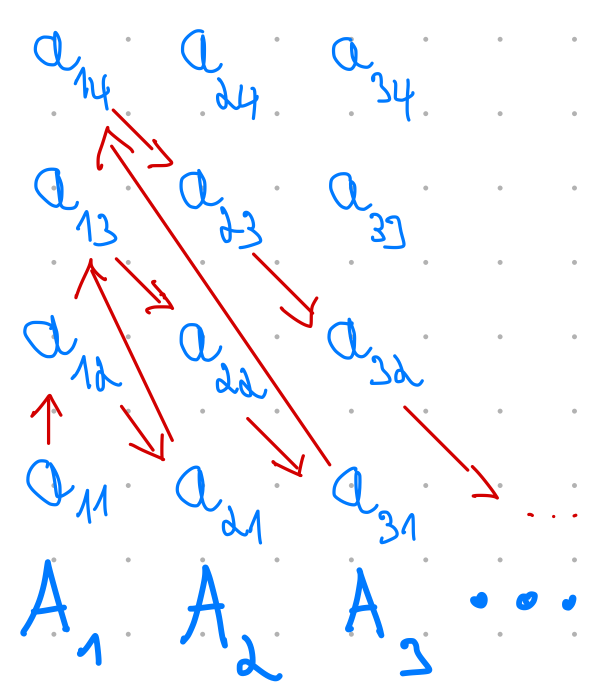
\includegraphics[height=5cm]{Img/zig-zag.png}
\caption{Argument Zig~-~Zag}\label{fig:zigzag}
\end{figure}
\end{proof}

L'énoncé de ce théorème peut se retenir de la manière suivante:
\begin{quotation}
\emph{Toute union dénombrable d'ensembles dénombrables est dénombrable.}
\end{quotation}

Nous avons mentionné (AC) en préalable à l'énoncé du Théorème \ref{thm:infinf}. Cela signifie que pour se théorème, nous devons supposer un axiome appelé l'\emph{axiome du choix}. Tout comme l'hypothèse du continu, il s'agit d'un indécidable de la théorie des ensembles: il n'es pas prouvable dans la théorie des ensembles et sa négation non plus. On peut donc soit supposer l'axiome du choix, soit sa négation (mais pas les deux) sans introduire de contradiction. La grande majorité des mathématiciens et mathématiciennes travaille en supposant l'axiome du choix. De nombreux théorèmes importants (comme l'existence d'une base dans les espaces vectoriels de dimension finie) sont en fait équivalent à l'axiome du choix, ou à une de ses formes faibles. Une formulation de l'axiome du choix est la suivante:
\begin{center}
Si $\{A_i \mid i \in I\}$ est une famille d'ensembles, alors il existe une fonction $f$ définie sur $I$ telle que $f(i)\in A_i$ pour tout $i\in I$.
\end{center}

\newpage

\section{Techniques de démonstration}

Qu'est-ce qu'une preuve? Il en existe de nombreux types qui dépendent du contexte dans lequel elles sont utilisées: preuve formelle en mathématiques, preuve d'identité en informatique, preuve judiciaire, preuve à divulgation nulle de connaissance\ldots~Dans tous les cas, \emph{prouver} c'est convaincre. Il s'agit en effet de convaincre son interlocuteur de l'exactitude d'une information, ou de sa véracité.

Évidement, nous allons uniquement nous concentrer sur les preuves en mathématiques. Là encore, il en existe de nombreux types. On distingue d'abord les preuves formelles dans des systèmes de déduction axiomatique (comme celui de la théorie des ensembles, mais il en existe aussi pour LPC, pour la logique du premier ordre ou pour d'autres systèmes de fondation comme la théorie des types qui revient sur le devant de la scène ces dernières années).

Ces preuves formelles sont très importantes car elle peuvent être vérifiées par un ordinateur. Mais nous sommes loin des preuves qui constituent l'activité journalière du/de la mathématicien·ne type, et qui sont au cœur de cette section.

Si on se réfère à Wikipedia\footnote{https://fr.wikipedia.org/wiki/Démonstration\_(logique\_et\_mathématiques) consulté le 25 juillet 2023 à 22:00 UTC+2.},
\begin{quotation}
 une \emph{preuve} ou \emph{démonstration} est un ensemble structuré d'étapes correctes de raisonnement. 
\end{quotation}
Cette définition informelle (et elle ne peut que rester informelle dès lors qu'on sort du cadre de la notion de preuve dans des systèmes axiomatiques) cache bien des réalités. Il y a de nombreuses techniques de preuves (nous en verrons les plus courantes), mais même en appliquant la même technique pour prouver la même assertion, des auteur·rice·s différent·e·s arriveront bien souvent à des expositions de preuves différentes, en fonction de leur expérience et de leur public cible. On ne présente pas une preuve de la même manière à un·e mathémticien·ne aguerri·e et à un·e élève de lycée.

Dans tous les cas, \emph{prouver} est la compétence majeure du/de la mathématicien·ne. Une telle compétence, cela se travaille! Lorsque vous rédigerez une preuve, vous n'y arriverez pas du premier coup. Il faudra d'abord tâtonner, écrire des bouts de raisonnement, tout effacer, restructurer et finalement exposer votre preuve dans votre meilleure prose mathématique. Le démonstration est l'écrin de la solution à l'énigme mathématiques que vous résolvez, et constitue un des meilleurs arguments de vente dans la communauté mathématique.

Qu'est-ce qui distingue une \emph{bonne preuve} d'une \emph{mauvaise preuve}\footnote{https://youtu.be/QuGcoOJKXT8?t=180}? Il y a sans doute autant de réponses à cette question qu'il n'y a de mathématicien·ne·s. Néanmoins, tous et toutes s'accordent à dire qu'une bonne preuve est
\begin{itemize}
\item rigoureuse (le raisonnement est valide et complet; si l'auteur applique un théorème dans la preuve, il en vérifie les hypothèses),
\item bien structurée (elle met en avant les étapes importantes de la démonstration; identifie les hypothèses et les thèses, et les techniques utilisées),
\item claire (elle ne laisse pas de place à l'interprétation ou au doute),
\item détaillée (elle ne laisse pas au lecteur un trop grand travail de vérification des assertions prouvées sans démonstration; le niveau de détails dépend évidement du public visé),
\item concise (elle ne présente pas d'arguments inutiles, hors sujets ou redondants),
\item et bien-sûr\ldots~correcte!
\end{itemize}
La critère de concision semble être en opposition avec celui du détail! C'est vrai, et une bonne preuve réalise un équilibre entre les deux. Pour simplifier, un·e mathématicien·ne essaye d'économiser les mots, sans sacrifier à la clarté et à la rigueur.

\subsection{Preuve directe}

Bien souvent, nous avons à démontrer une assertion du type \emph{Si $A$ alors $B$}, c'est à dire $A \iimplies B$ où $A$ et $B$ sont des assertions quelconques. La technique la plus élémentaire, c'est de montrer que cette implication est vrai en recourant à la table de connecteur de $\iimplies$.

Pour une \emph{preuve directe},
\begin{quotation}
\emph{sous l'hypothèse que $A$ est une assertion vraie, on prouve que l'assertion $B$ est aussi vraie.}
\end{quotation}
Donnons un exemple de preuve directe.
\begin{example}\label{ex:dir}
\emph{Si $n$ est un entier pair alors $n^2$ est pair.} 
\end{example}
\begin{proof}
Prouvons cette assertion par preuve directe. Supposons que $n$ est un entier pair. Alors, il existe par définition un entier $k$ tel que $n=2k$. On a donc successivement
\[
n^2=(2k)^2=4k^2=2(2k^2),
\]
où la deuxième égalité est vraie pour commutativité de la multiplication dans $\Z$ et la dernière égalité s'obtient par associativité de la multiplication.
\end{proof}
\begin{remark}
Dans cette preuve, nous avons justifié les égalités par des propriétés élémentaires de la multiplication. Quand bien même nous n'aurions pas écrit ces justifications, vous auriez accepté la démonstration comme valide, car vous manipulez ces propriétés avec aisance. Par contre, un jeune élève de l'enseignement secondaire aurait peut-être bien eu besoin des justifications pour suivre le raisonnement. L'exemple illustre bien que la manière d'\emph{exposer} une preuve dépend du public cible auquel elle va être présentée, même si sa validité mathématique en est indépendante.
\end{remark}

\subsection{Preuve par contraposition}
Nous avons vu qu'une implication $A \iimplies B$ est équivalente à sa contraposée $\neg B  \iimplies \neg A$. Pour prouver un énoncé du type 
\begin{quotation}
Si $A$ alors $B$,
\end{quotation}
il est donc équivalent de prouver 
\begin{quotation}
Si $\neg B$ alors $\neg A$.
\end{quotation}
On dit qu'on procède par \emph{contraposition}, ou bien que l'on prouve \emph{la contraposée}. Cela peut paraître étonnant, mais parfois prouver la contraposée s'avère plus facile que prouver l'énoncé original. Donnons un exemple.
\begin{example}
\emph{Soit $q$ un nombre réel positif. Si $q$ est irrationnel alors $\sqrt{q}$ est irrationnel.}
\end{example} 
\begin{proof}
Procédons par contraposition et supposons que $q$ est un nombre réel positif tel que $\sqrt{q}$ est rationnel. Nous devons en déduire que $q$ est rationnel. Par hypothèse, il existe $m,n \in \Z$ tels que $n\neq 0$ et $\sqrt{q}={m}/{n}$. En élevant cette identité au carré, on en déduit que $q={m^2}/{n^2}$. Nous avons écrit $q$ comme le quotient de deux nombres entiers, ce qui prouve que $q$ est rationnel. On conclut la preuve par le principe de contraposition.
\end{proof}

\begin{remark}
Dans la preuve précédente, nous avons écrit
\begin{quotation}
Il existe $m,n \in \Z$ tels que $n\neq 0$ et $\sqrt{q}={m}/{n}$. En élevant cette identité au carré, on en déduit que $q={m^2}/{n^2}$
\end{quotation}
Cette assertion signifie en langage symbolique
\[
\exists m,n \in \Z \big((n\neq 0\wedge \sqrt{q}={m}/{n})\iimplies q={m^2}/{n^2}\big).
\]
C'est-à-dire que \og~on en déduit~\fg{} se traduit par une implication $\iimplies$ et pas par une équivalence $\Leftrightarrow$. C'est une remarque importante car l'équivalence est fausse dans notre cas\footnote{Pourquoi? Et comment aurait-on pu reformuler l'assertion pour avoir une équivalence?}. \emph{La terminologie utilisée pour structurer la preuve est donc d'une importance capitale, puisqu'une erreur peut invalider la démonstration}. 
\end{remark}

\subsection{Preuve d'une équivalence}

Pour prouver une équivalence entre deux assertions, rien de plus simple (en tout cas du point de vue de la structure de la preuve). En effet, rappelons que l'assertion $\varphi \ifff \psi$ est en fait une abréviation de $(\varphi \iimplies \psi) \wedge (\psi \iimplies \varphi)$. Prouver $\varphi \ifff \psi$ est donc équivalent  à prouver les deux assertions  $(\varphi \iimplies \psi)$, $(\psi \iimplies \varphi)$.

\begin{example}
\emph{Pour tout entier $z\in \Z$, on a $z$ est impair si et seulement si $z^2$ est impair}
\end{example}
\begin{proof}
(Nécessité) Supposons que $z$ est impair et déduisons-en que $z^2$ est impair. Nous savons qu'il existe $k\in \Z$ tel que $z=2k+1$. En élevant au carré et en développant, on obtient 
\[
z^2=(2k+1)^2=4k^2+4k+1=2(2k+2)+1.
\]
Ainsi, $z^2-1=2(2k+2)$ est un multiple de 2, c'est-à-dire que $z^2$ est impair.

(Suffisance) Supposons que $z^2$ est impair et déduisons-en que $z$ est impair. Il suffit de prouver la contraposée, à savoir que si $z$  est un entier pair alors $z^2$ est une entier pair. Cette preuve a été faite dans l'Exemple \ref{ex:dir}.
\end{proof}

\begin{remark}
L'assertion à démontrer dans l'exemple précédent prenait la forme $\varphi \ifff \psi$ où $\varphi$ est l'assertion \emph{$z$ est impair} et $\psi$ l'assertion \emph{$z^2$ est impair}. Dans la première partie de la preuve intitulée \og~Nécessité~\fg{}, nous avons démontrer que l'assertion $\varphi \iimplies \psi$ est vraie, et dans la deuxième partie de la preuve intitulée \og~Suffisance~\fg, nous avons démontrer que l'assertion $\psi  \iimplies \varphi$ est vraie. Bien que d'un point de vue logique l'expression $\varphi \ifff \psi$ est symétrique, lorsque nous structurons une preuve de cette équivalence, nous considérons donc une asymétrie (parfaitement justifiée par le fait que la \emph{syntaxe} $\varphi \ifff \psi$, elle, n'est pas symétrique). En effet, $\varphi$ est considérée comme assertion \og~de référence~\fg{} par rapport à laquelle on compare $\psi$: dans la première partie $\psi$ est qualifiée de condition \emph{nécessaire} (sous-entendu \emph{à $\varphi$}) et dans la deuxième, de condition \emph{suffisante} (sous-entendu à $\varphi$).

Au lieu du terme \og~Néssecité~\fg{}, on peut utiliser une terminologie alternative, comme l'une des suivantes 
\begin{quotation}
\noindent (${\Longrightarrow}$)\\
\emph{Prouvons l'implication de gauche à droite [\ldots]}\\
\emph{Prouvons que $\varphi$ implique $\psi$ [\ldots]}	
\end{quotation}
Similairement, au lieu du terme \og~suffisance~\fg{}, on peut utiliser une terminologie alternative, comme l'une des suivantes 
\begin{quotation}
\noindent (${\Longleftarrow}$)\\
\emph{Prouvons l'implication de droite à gauche [\ldots]}\\
\emph{Prouvons que $\psi$ implique $\varphi$ [\ldots]}	
\emph{Prouvons la réciproque [\ldots]}
\end{quotation}
\end{remark}

Parfois, il est aussi simple de démontrer l'équivalence $\varphi \iff \psi$ en prouvant les deux implications $\varphi \iimplies \psi$ et $\psi \iimplies \psi$ \emph{en même temps}, c'est-à-dire par une suite d'équivalence\footnote{On utilise implicitement pour cela la transitivité de l'implication, à savoir le fait que l'assertion $(\varphi \iimplies \psi) \iimplies  ((\psi \iimplies \rho)\iimplies (\varphi \iimplies \rho))$ est une tautologie (bien connue des enfants au travers de la chanson \emph{Biquette}~.)}. Donnons un exemple.
\begin{example}
Soit $x\in \R$. On a $\sqrt{(x-1)^2+(y-3)^2}=0$ si et seulement si ($x=1$ et $y=3$).
\end{example}
\begin{proof}
On obtient les équivalences successives suivantes.
\begin{align}
\sqrt{(x-1)^2+(y-3)^2}=0 & \iff (x-1)^2+(y-3)^2=0\label{eqn:zer01}\\
& \iff (x-1)^2=0 \wedge (y-3)^2=0\label{eqn:zer02}\\
& \iff (x-1)=0 \wedge (y-3)=0\label{eqn:zer03}\\
& \iff x=1 \wedge y=3,\label{eqn:zer04}
\end{align}
où \eqref{eqn:zer01} et \eqref{eqn:zer03} sont obtenus parce qu'un nombre réel est nul si et seulement si son carré est nul, et \eqref{eqn:zer02} parce que la somme de deux nombres positifs est nul si et seulement si ils sont tous les deux nuls.
\end{proof}

Parfois, on est amené à prouver que plusieurs assertions sont mutuellement équivalentes, comme dans l'exemple suivant. Dans ce cas, on peut à nouveau se servir de la transitivité de l'implication et se compter de prouver un cycle d'implication qui contient toutes les assertions.
\begin{example}
\emph{Pour tout nombre réel $x$, les conditions suivants sont équivalentes.
\begin{enumerate}[(i)]
\item $\sqrt{x^2}=x$.
\item $|x|=x$.
\item $x\geq 0$.
\end{enumerate}}
\end{example}
\begin{proof}
(i)$\implies$(iii) Par définition, pour un nombre positif $y$, le nombre $\sqrt{y}$ est l'unique nombre positif donc le carré vaut $y$. Ainsi, si $\sqrt{x^2}=x$ alors $x$ est positif.

(iii)$\implies$(ii) Par définition, on a
\[
|x| = \left\{\begin{array}{ll}
x & \text{ si } x\geq 0\\
-x & \text{ si } x< 0.
\end{array}\right.
\]
En particulier, si $x\geq 0$ alors $|x|=x$.

(ii) $\implies$ (i) On a toujours $\sqrt{y^2}=|y|$. Donc si $|x|=x$, on a $\sqrt{x^2}=|x|=x$.

Au total on a prouvé (i) $\iimplies$ (iii) $\iimplies$ (ii) $\iimplies$ (i), donc toutes ces conditions sont équivalentes.
\end{proof}

\subsection{Preuves par cas}

Parfois, la preuve directe d'une implication $\varphi \implies \psi$ ne se fait pas en une seule suite d'implications, mais on sépare la preuve en différents cas mutuellement exclusifs, comme dans l'exemple ci-dessous.
\begin{example}
\emph{Si $n\in \N$ alors $1+(-1)^n(2n-1)$ est un multiple de 4}.
\end{example}
\begin{proof}
Si $n\in \N$ alors soit $n$ est pair, soit $n$ est impair, mais pas les deux.

\noindent{\bfseries Cas 1. } \emph{Supposons que $n$ est pair}. Il existe $k\in \Z$ tel que $n=2k$. Il vient successivement
\[
1+(-1)^n(2n-1)=1+(-1)^{2k}(4k)-1=1+4k-1=4k,
\]
qui est un multiple de $4$.

\noindent{\bfseries Cas 2. } \emph{Supposons que $n$ est impair}. Il existe $k\in \Z$ tel que $n=2k+1$. Il vient successivement
\[
1+(-1)^n(2n-1)=1+(-1)^{2k+1}(2(2k+1)-1)=1-(4k+2-1)=-4k,
\]
qui est un multiple de 4.

Les deux cas prouvent que $1+(-1)^n(2n-1)$ est toujours un multiple de 4.
\end{proof}
\begin{remark}
Dans une preuve par cas, il faut bien faire attention à couvrir tous les cas possibles, sous peine de produire une preuve invalide. Les cas ne doivent pas nécessairement être exclusifs, mais leur disjonction doit couvrir la situation la plus générale. 
\end{remark}

\subsection{Preuve de la négation}
Nous avons déjà remarqué que la négation $\neg A$ d'une assertion $A$ est équivalente à $A \iimplies  \bot$. Pour prouver que $\neg A$ esr vrai, il est donc équivalent de prouver
\begin{quotation}
Si $A$ est vrai alors on en déduit une contradiction.
\end{quotation}
Donnons un exemple célèbre, connu depuis l'antiquité.

\begin{example}
$\sqrt{2}$ n'est pas rationnel.
\end{example}
\begin{proof}
Prouvons que $(\sqrt{2} \in \Q) \iimplies \bot$. Supposons que $\sqrt{2}\in \Q$, c'est-à-dire qu'il existe deux entiers positifs $m$ et $n$ qui n'ont pas de diviseur commun, tels que $n\neq 0$ et $\sqrt{2}=m/n$. On obtient successivement
\begin{align}
\sqrt{2}=m/n & \ifff 2=m^2/n^2 \label{eq:kju00}\\
 & \ifff 2n^2=m^2\label{eq:kju01}\\
 & \iimplies m^2 \text{ est pair }\label{eq:kju02}\\
 & \iimplies m \text{ est pair }.\label{eq:kju03}
\end{align}
Il existe donc $k\in \N$ tel que $m=2k$. L'identité (\ref{eq:kju01}) est donc équivalence à 
$
2n^2=4k^2
$, c'est-à-dire à $n^2=2k^2$. On en déduit que $n^2$ est pair, donc $n$ l'est aussi. On a obtenu que $m$ et $n$ sont des multiples de deux, ce qui contredit le fait que $m$ et $n$ n'ont pas de diviseur commun. Nous avons prouvé que $\sqrt{2}\not \in \Q$.
\end{proof}
\begin{remark}
\begin{enumerate}
\item Pour obtenir (\ref{eq:kju02}), nous avons à nouveau élever l'identité $\sqrt{2}=m/n$ au carré. Nous obtenons cette fois une équivalence (par opposition à une implication dans la preuve précédente) car nous avons supposé que $m$ et $n$ étaient positifs.
\item La relation (\ref{eq:kju02}) n'est qu'une implication, et nous l'avons identifié comme tel (la réciproque est fausse).
\item En revanche, on peut montrer (exercice) que la réciproque de (\eqref{eq:kju03}) est vraie. Comme la réciproque ne nous sert pas à la preuve, nous ne l'avons pas indiqué comme tel, ce qui nous permet d'en économiser la preuve.
\end{enumerate}
\end{remark}

\subsection{Preuve par contradiction}
Le principe de \emph{preuve pas contradiction} (ou de \emph{preuve par l'absurde}) s'énonce comme ceci:
\begin{quotation}
Si $\varphi$ n'est pas faux, alors $ \varphi$ est vrai.
\end{quotation}
Sa validité est ancrée dans le principe du tiers-exclu $\varphi \vee \neg \varphi$. Formellement, il s'énonce donc comme
\[
\neg\neg \phi \iimplies \phi,
\]
ou encore 
\[
(\neg \phi \iimplies \bot) \implies \phi,
\]
qui est équivalent au tiers-exclu $\phi \vee \neg \phi$.
Pour l'utiliser pour démontrer une assertion $\phi$, on procède donc en deux étapes.
\begin{enumerate}[(1)]
\item On suppose $\neg \phi$ et on en déduit une contradiction $\bot$. C'est-à-dire qu'on a démontré $\neg \phi \iimplies \bot$, à savoir $\neg\neg \phi$
\item Par le principe de contradiction $\neg\neg \phi \iimplies \phi$, on en déduit $\phi$.
\end{enumerate}

Donnons un exemple archétypal, connu depuis l'antiquité grecque (depuis Euclide, pour être plus précis). Rappelons qu'un entier naturel $n>1$ est qualifié de \emph{nombre premier} s'il n'est divisible que par 1 et par $n$. Pour le moment, nous acceptons sans preuve le résultat suivant (nous le prouverons plus tard, dans la section relative aux relations d'ordre)
\begin{lemma}\label{lem:prem}
Tout entier naturel $n>1$ qui n'est pas premier est divisible par un nombre premier\footnote{C'est-à-die que pour tout naturel $n>1$ qui n'est pas premier, il existe un nombre premier $p\neq n$ qui divise $n$.}.
\end{lemma}

C'est sous la forme de sa contraposée \emph{si $n>1$ est un naturel qui n'est divisble par aucun nombre premier $p$ différent de $n$ alors $n$ est premier} que nous allons utiliser le lemme précédent.

\begin{theorem}
Il existe une infinité de nombres premiers.
\end{theorem}
\begin{proof}
Procédons par contradiction. Supposons que l'ensemble $A$ des nombres premiers soient fini, et que $p_1, p_2, \ldots, p_\ell$ soit une liste de tous les éléments de $A$ (on a donc $\ell\geq 2$). Définissons le nombre $p\in \N$ comme
\[
p:=p_1p_2\cdots p_\ell+1.
\]
Comme $\ell\geq 2$, on sait que $p>\max\{p_i \mid i \leq \ell\}>1$. De plus, on sait que $p-1$ est un multiple de $p_i$ pour tout $i\leq \ell$, donc $p$ n'est pas un multiple de $p_i$. Ainsi, $p>1$ qui n'est pas premier (puisqu'il est différent de $p_1, \ldots, p_\ell$) mais qui n'est pas divisible par un nombre premier. C'est en contradiction avec le Lemme \ref{lem:prem}. Par le principe de contradition, on conclut que l'ensemble des nombres premiers $A$ est infini.
\end{proof}
\begin{further}{Preuve de la négation et principe de contradiction}
En y regardant bien, une preuve de $\neg \varphi$ qui consiste en ceci:
\begin{quotation}\itshape
Supposons $\varphi$ et déduisons une contradiction $\bot$
\end{quotation}
ressemble fort au début d'un preuve par  contradiction de $\varphi$:
\begin{quotation}\itshape
Supposons $\neg \varphi$ et déduisons une contradiction $\bot$.
\end{quotation}
Évidement, ce n'est qu'une ressemblance: d'un côté on veut prouver $\neg \varphi$ et de l'autre on veut prouver $\varphi$. Mais la différence est beaucoup plus profonde. En effet, en procédant à la preuve de $\neg \varphi$, on procède par une preuve directe de $\neg \phi$ \emph{qui est indépendant de la règle du tiers-exclus $\psi \vee \neg \psi$.} Tandis que le principe de contradiction est \emph{équivalent au tiers-exclus.}
\smallskip

Or, la règle du tiers-exclu est d'un statut particulier: elle permet d'affirmer que $\varphi$ est vrai simplement parce que $\neg \varphi$ n'est pas vrai, donc sans avoir \emph{obtenu une preuve directe de $\varphi$}. Les résultats mathématiques qu'on peut obtenir \emph{sans utiliser le tiers-exclus} (donc sans le principe de contradiction qui lui est équivalent) sont appelés \emph{constructifs}, et on parle de \emph{mathématiques constructives}. 
\smallskip

Il y a des résultats mathématiques fondamentaux qu'il est \emph{impossible d'obtenir de manière constructive}, comme l'existence d'une base dans les espaces vectoriels de dimension infinie. Plus généralement, tous les résultats qui dépendent de l'\emph{Axiome du choix} sont non constructifs (l'axiome du choix est en fait \emph{équivalent} au tiers-exclus). Dans votre \emph{cursus}, vous découvrirez le \emph{Prime Ideal Theorem}, le Théorème de Tychonoff (tout produit d'espaces compacts est compacts), le Théorème de Hahn~-~Banach qui dépendent tous de l'Axiome du choix. 
\smallskip

Pourquoi faire une telle distinction entre \emph{mathématiques constructives} et \emph{mathématiques non-constructives}? Acceptons d'utiliser le tiers-exclus (c'est ce qu'on va faire) et oublions tout cela. C'est vrai, mais gardons dans le coin de notre tête que le tiers-exclus, via son équivalent l'axiome du choix, permet aussi d'énoncer des résultats contre-intuitifs comme le \og~pardoxe~\fg{} de Banach~-~Tarski: \emph{il est possible de découper une boule de l'espace usuel $\mathbb{R}^{3}$ en un nombre fini de morceaux et de réassembler ces morceaux pour former deux boules identiques à la première, à un déplacement près.}\footnote{Source: \url{https://fr.wikipedia.org/wiki/Paradoxe_de_Banach-Tarski} consultée le 31 juillet 2023 à 15:15 UTC+2.} La clé pour déjouer le paradoxe apparent est que les morceaux en questions sont \emph{non mesurables}.
\end{further}

\subsection{Preuves par induction}
Supposons avoir une suite d'assertions $\varphi_0, \varphi_1, \ldots \varphi_n, \ldots$ de nature \og~similaires~\fg{}, comme par exemple la suite $(\varphi_n)_{n\in \N}$ dont le $n^{e}$ terme est l'assertion \[\sum_{i=0}^ni=n(n+1)/2.\]
La technique de \emph{preuve par induction} ou \emph{par récurrence} consiste en ceci:
\begin{quotation}
Pour prouver que toutes les assertions $\varphi_0, \varphi_1, \ldots $ sont vraies, il suffit
\begin{enumerate}[(1)]
\item De prouver que $\varphi_0$ est vrai.
\item De prouver que si pour un $n$ donné l'assertion $\varphi_n$ est vraie, alors l'assertion $\varphi_{n+1}$ est vraie.
\end{enumerate}
\end{quotation} 

En effet, par (1) on sait que $\phi_0$ est vrai. Par (2) appliqué avec $n=0$, on sait que $S_1$ est vrai. Par (2) appliqué avec $n=1$, on sait que $S_2$ est vrai\ldots Ainsi, le principe d'induction (qui peut être formellement défini en théorie des ensembles) permet d'obtenir une infinité (dénombrable) de résultats en en prouvant un nombre fini.

Dans une preuve par récurrence, on appelle l'étape (1) le \emph{cas de base} et l'étape (2) \emph{l'étape de récurrence}. Dans cette étape, l'hypothèse $\varphi_n$ sous laquelle on travaille s'appelle \emph{hypothèse de récurrence}, que nous noterons (HR).

%\begin{further}{Principe d'induction: magie ou mathématiques?}
%Ce tour de force mathématique qu'est le principe d'induction a conduit Henri Poincaré [;;;\ldots;;;]
%\end{further}

Donnons en tout de suite un exemple.

\begin{proposition}
Pour tout entier naturel $n$ on a 
\[
\sum_{i=0}^n i =\frac{n(n+1)}{2}.
\]
\end{proposition}
\begin{proof}
Pour tout $n\geq 0$ désignons par $\varphi_n$ l'assertion ${\sum}_{i=0}^n\ i =\frac{n(n+1)}{2}$. Prouvons par récurrence que pour tout $n\geq 0$ l'assertion $\varphi_n$ est vraie.

Prouvons le cas de base $\varphi_0$. D'une part on a ${\sum}_{i=0}^0\ i =0$, d'autre par  ${0(0+1)}/{2}=0$, ce qui prouve $\varphi_0$.

Démontrons maintenant l'étape de récurrence, et supposons (HR) que $n\geq 0$ est un naturel pour lequel $\varphi_n$ est vrai, à savoir
\begin{equation}\label{eqn:mpos}
\sum_{i=0}^n\ i =\frac{n(n+1)}{2}\tag{HR}
\end{equation}
Prouvons que $\varphi_{n+1}$ est vrai, à savoir \[\sum_{i=0}^{n+1}\ i =\frac{(n+1)(n+2)}{2}.\]

Il vient successivement
\begin{align}
\sum_{i=0}^{n+1}\ i & = \sum_{i=0}^{n}\ i +(n+1)\\
 & = \frac{n(n+1)}{2}+(n+1)\label{eqn:gfr01}\\
 & = \frac{(n+1)(n+2)}{2}\label{eqn:gfr02},
\end{align}
où \eqref{eqn:gfr01} est obtenu en appliquant l’hypothèse d'induction (HR), et \eqref{eqn:gfr01} par mise en évidence de $(n+1)$ et addition des fractions. Nous avons bien obtenu \eqref{eqn:mpos}. On conclut la preuve par le principe d'induction.
\end{proof} 
\begin{remark}
\begin{enumerate}
\item Dans une preuve par récurrence, prouver le cas de base est \emph{indispensable}. Il sert de socle au raisonnement. Il est possible d'énoncer des suites $\varphi_0, \varphi_1\ldots$ d'assertions pour lesquelles on peut prouver l'étape de récurrence \emph{mais pas le cas de base}. Pour ces assertions, le principe d'induction ne s'applique pas.
\item Si vous arrivez à prouver l'étape d'induction \emph{sans faire appel à l'hypothèse d'induction}, c'est que vous avez fait une erreur. Arrêtez-vous et éliminez la.
\item Parfois, la suite d'assertions que l'on souhaite prouver commence à $n=1$ et est tu type $\varphi_1, \varphi_2\ldots$. Dans ce cas, le cas de base est $\varphi_1$, et l'étape de récurrence consiste à supposer que $\varphi_n$ est vrai pour un certain $n\geq 1$ et à en déduire $\varphi_{n+1}$. De même, cette suite commence parfois à $n=2$ ou \ldots
\item Il existe une version plus forte du principe de récurrence, qui consiste à prouver l'étape de récurrence de la manière suivante:
\begin{quotation}
 Supposons que pour un $n\geq 0$, les assertions $\varphi_0, \varphi_1 \ldots,  \varphi_n$ sont vraies et déduisons-en $\varphi_{n+1}$.
\end{quotation}
 
\end{enumerate}
\end{remark}

Donnons encore un très intéressant exemple d'application du principe d'induction: les tours de Hanoï.

\begin{example}[Tours de Hanoï]
Considérons le célèbre casse-tête des \emph{Tours de Hanoï}, inventé par le mathématicien Édouard Lucas à la fin du XIXe siècle. Un nombre $n \geq 1$ de disques de taille strictement décroissante (du haut vers le bas) sont placés sur une tour. Vous devez déplacez ces disques pour former une nouvelle tour finale, en utilisant une tour auxiliaire et en respectant les règles suivantes (voir aussi la Fig.~\ref{fig:han}):
\begin{enumerate}
\item vous ne pouvez déplacer qu'un disque à la fois;
\item vous ne pouvez pas placer un disque sur un disque plus petit que lui.
\end{enumerate}

\emph{Quel est le nombre minimum  de déplacements de disques à effectuer pour déplacer la tour?}
\begin{figure}\centering
\begin{tikzpicture}[scale=0.5]
\foreach \i in {1,2,...,5}
{
\draw (-\i/2, 5/3-\i/3) rectangle +(\i, 1/3);
}
\draw[thick] (0,0) -- (0, 2.5);
\draw (0,0) node[below]{$A$};
\draw[thick] (5,0) -- (5, 2.5);
\draw (5,0) node[below]{$B$};
\draw[thick] (10,0) -- (10, 2.5);
\draw (10,0) node[below]{$C$};
\end{tikzpicture}\caption{Tours de Hanoï}\label{fig:han}
\end{figure}
\end{example}
\begin{proof}[Solution]
Définissons un algorithme récursif\footnote{Un \emph{algorithme récursif} est un algorithme qui résout un problème en calculant des solutions d'instances plus petites du même problème. Source: \url{https://fr.wikipedia.org/wiki/Algorithme_r\%C3\%A9cursif} consulté le 1 août 2023 à 10:32  } $\mathsf{Han}(n, A, C, B)$ pour déplacer la tour de $n\geq 0$ disques de l'emplacement $A$ à l'emplacement $C$ (dans la Fig.~\ref{fig:han}) en utilisant l'emplacement auxiliaire $B$:
\begin{quotation}
\noindent Si $n=0$, ne rien faire; sinon
\begin{enumerate}
\item déplacer les $n-1$ premiers disques de l'emplacement $A$ à l'emplacement $B$ en utilisant l'algorithme $\mathsf{Han}(n-1, A, B, C)$;
\item déplacer le disque de taille $n$ de la tour $A$ à la tour $C$;
\item déplacer les $n-1$ disques de l'emplacement $B$ à l'emplacement $C$ en utilisant l'algorithme $\mathsf{Han}(n-1, B, C, A)$.
\end{enumerate}
\end{quotation}
Désignons par $(H_n)_{n\in \N}$ la suite dont le $n^{e}$ terme est le nombre de déplacements de disques effectués par $\mathsf{Han}(n,A,C,B)$. 
\begin{figure}
\[\begin{array}{c|c}
n & H_n\\ \hline
0 & 0\\
1 & 1\\
2 & 3\\
3 & 7\\
4 & 15\\
\cdots & \cdots
\end{array}\]
~\caption{Valeurs des premiers termes de $(H_n)_{n\in  \N}$}\label{fig:hannb}
\end{figure}
Nous allons en fait prouver l'assertion suivante:
\begin{quotation}\itshape
Pour tout $n\geq 0$ on a $H_n=2^{n}-1$ mouvements. De plus, l'algorithme $\mathsf{Han}(n,A,C,B)$ est optimal, dans le sens où il n'existe pas d'autres algorithme qui déplacerait les $n$ disques en $m$ mouvements avec $m<n$.
\end{quotation}
Tout d'abord, prouvons l'identité
\begin{equation}\label{eqn:dfm}
H_n=2^n-1,\qquad n\geq 0,
\end{equation}
par récurrence sur $n$. Nous avons déjà démontré le cas de base, à savoir que $H_0=0$. Passons à  l'étape de récurrence et supposons (HR) que $H_n=2^{n}-1$ pour un $n\geq 0$ donné. Prouvons sous l'hypothèse (HR) que
\begin{equation}\label{eqn:dvf}
H_{n+1}=2^{n+1}-1.
\end{equation}
En appliquant la définition de l'algorithme, on constate que
\[
H_{n+1} = H_n+1+H_n
\]
car il faut $H_n$ mouvements pour réaliser l'étape 1 de l'algorithme, de même pour l'étape 3 et un seul mouvement pour l'étape 2. On appliquant l'hypothèse de récurrence (HR) on a donc
\[
H_{n+1}=2H_n+1=2(2^n-1)+1=2^{n+1}-1,
\]
et on obtenu l'identité \eqref{eqn:dvf}. On conclut que l'assertion \eqref{eqn:dfm} tient par le principe d'induction.
\smallskip

Prouvons maintenant que l'algorithme $\mathsf{Han}(n,A,C,B)$ est optimal, en procédant pas récurrence sur $n$. Le cas de base $n=0$ est trivial: l'algorithme $\mathsf{Han}(n,A,C,B)$ déplace 0  disque en 0 mouvement, c'est optimal.

Supposons maintenant (HR) que l'algorithme déplace de manière optimale une tour de $n$ disques pour une valeur de $n$ fixée, et prouvons que $\mathsf{Han}(n+1,A,C,B)$ déplace $n+1$ disques de manière optimale, c'est-à-dire que tout autre algorithme déplacerait les disques en $H_{n+1}$ mouvements \emph{au moins}. En effet, cet autre algorithme doit d'abord déplacer les $n$ premiers disques de $A$ à $B$, ce qui utiliser au moins $H_n$ mouvements (on utilise ici l'hypothèse de récurrence). Ensuite il doit déplacer le plus grand disque en 1 mouvement, puis à nouveau les $n$ disques de la tour $B$ à la tour $C$ en au moins $H_n$ mouvements (par HR,à nouveau). Au total, cet autre algorithme effectue au moins $2H_n+1=H_{n+1}$ mouvements.

On conclut que l'algorithme $\mathsf{Han}(n,A,C,B)$ est optimal pour tout $n\geq 0$ par le principe d'induction.
\end{proof}

L'exemple suivant illustre qu'un brin d'étourderie peut être désastreux dans une preuve par récurrence (comme dans toute preuve, d'ailleurs).
\begin{example}
Voici une tentative de preuve de l'assertion \emph{Dans ton groupe de $n$ personnes (pour $n\geq 1$), tous les individues ont la même couleur d'yeux.}
\end{example}

Pour conclure cette section, notons qu'il est également d'usage courant en mathématiques de \emph{définir} une suite $(A_n)$ d'objets mathématiques (ensembles, nombres, espaces, structures\ldots) par récurrence. L'idée est de définir le premier terme $A_0$ de la suite, et de donner une règle de construction du $(n+1)^{e}$ terme à partir du $n{e}$ terme (ou des termes $A_0$ à $A_n$). L'avantage est de pouvoir utiliser cette définition par récurrence pour prouver, par récurrence, des assertions à propos de cette suite.

\begin{example}
Définissons une suite d'ensembles $(A_n)_{n\in \N}$ par récurrence par
\[
A_n= \left\{\begin{array}{cl}
\varnothing & \text{ si } n=0,\\
\mathcal{P}(A_{n-1}) & \text{ si } n\geq 1.
\end{array}\right.
\]
\emph{Démontrer par récurrence (exercice) que pour tout $n\geq 0$ on a $\#A^n=2^n$}
\end{example}

\begin{exercise}[Factorielle]
On définit la fonction \emph{factorielle} $\cdot!\colon \N \to \N$ par induction en suivant les règle suivantes:
\[
n!:=\left\{
\begin{array}{ll}
1 & \text{ si } n=0\\
n\times (n-1)! & \text{ si } n\geq 1.
\end{array}
\right.
\]
\emph{Prouver par récurrence sur $n\geq 0$ que $n!$ est égal au produit de $n$ premiers entiers naturels.}
\end{exercise}


\subsection{Contre-exemple et preuve de la négation}

Quand ils sont exprimés dans le langage naturel (en anglais, français\ldots) les énoncés mathématiques prennent souvent la forme
\begin{quotation}
Si $\varphi(x_1, \ldots, x_\ell)$ alors $\psi(x_1, \ldots, x_\ell)$,
\end{quotation}
où $\varphi(x_1, \ldots, x_\ell)$ et $\psi(x_1, \ldots, x_\ell)$ sont des assertions à plusieurs variables (qui peuvent être de type différent: nombres, fonctions\ldots). Une telle assertion est en fait une traduction en langage naturel de l'assertion 
\[
\forall x_1, \ldots, x_\ell \ (\varphi(x_1, \ldots, x_\ell) \iimplies \psi(x_1, \ldots, x_\ell)).
\]
 Cela signifie que si nous souhaitons montrer que l'assertion est fausse, nous devons prouver 
 \[
 \exists x_1, \ldots, x_\ell \ \varphi(x_1, \ldots, x_\ell) \wedge \neg \psi(x_1, \ldots, x_\ell).
\]
Il s'agit donc de trouver un \emph{contre-exemple} (ou \emph{contre-modèle}, c'est-à-dire une interprétation des variables $x_1, \ldots, x_\ell$ telle que $\varphi(x_1, \ldots, x_\ell)$ est vrai mais $\psi(x_1, \ldots, x_\ell)$ est faux.

\begin{example}
Démontrez que l'assertion 
\begin{quotation}
\emph{Si $A_1$ et $A_2$ sont des ensembles alors $\#(A_1 \cup A_2)=\#A_1 \cup \#A_2$.}
\end{quotation}
est fausse.
\end{example}
\begin{proof}[Solution]
Nous en donnons un contre-exemple. Si $A_1$ désigne l'ensemble $\{1,2\}$ et $A_2$ désigne l'ensemble $\{2,3\}$ alors $\#(A_1 \cup A_2)=3$ alors que $\#A_1 \cup \#A_2=4$.
\end{proof}

\begin{further}{Pour s'entraîner}
Produire des preuves est le cœur de métier du mathématicien et de la mathématicienne. Pour s'entraîner ou en découvrir d'avantage, les lecteur·rice·s peuvent se référer à \cite{Hammack2003}
\end{further}

\section{Équivalence}

Imaginons que vous étudiez la géométrie dans le plan, et que vous vous intéressiez aux triangles. Voici trois triangles dans le plan
\begin{center}
\begin{tikzpicture}

% Triangle A (with angles 60°, 40°, and 80°)
\coordinate (A1) at (0,0);
\coordinate (A2) at (2,0);
\coordinate (A3) at (1,2);
\draw (A1) -- (A2) -- (A3)--(A1);

\coordinate (B1) at (4,0);
\coordinate (B2) at (4,2);
\coordinate (B3) at (6,1);
\draw (B1) -- (B2) -- (B3)--(B1);

\coordinate (C1) at (8,0);
\coordinate (C2) at (9,1);
\coordinate (C3) at (12,1.5);
\draw (C1) -- (C2) -- (C3)--(C1);
\end{tikzpicture}
\end{center}
Il s'agit là de trois triangles différents (en tant qu'ensemble de points du plan). Néanmoins, face à ces triangles, un enfant vous dira que les deux premiers sont identiques, mais que le troisième est différent des autres. On peut en effet superposer les deux premiers triangles parfaitement, mais pas avec le troisième.

Pour capturer cette notion de triangles \og~identiques~\fg, les mathématicien·ne·s ont introduit la notion d'isométrie, que vous avez découverte dans l'enseignement secondaire. Les deux premiers triangles sont isométriques, mais ne sont pas égaux. Dans le géométrie du triangle, ce n'est pas la notion d'égalité qui est pertinente pour comparer les triangles, mais le notion d'isométrie. Nous ne sommes pas intéressés à distinguer des triangles qui sont isométriques car ils ont les mêmes propriétés géométriques: ils sont équivalents du point de vue de la géométrie.

Une telle identification est monnaie courante en mathématique. On pourrait même grossièrement résumer l'activité mathématique à la classification des \og~motifs~\fg{} à une forme d'équivalence prêt.

Dans cette section, nous donnons un sens mathématique à la notion d'équivalence, et à celle de quotient qui va de pair.

\begin{definition}
Une relation binaire $R$ sur un ensemble $X$ est une \emph{équivalence} (ou une \emph{relation d'équivalence}) si
\begin{itemize}
\item elle est \emph{réflexive}, c'est-à-dire $xRx$ pour tout $x\in X$;
\item elle est \emph{symétrique}, c'est-à-dire pour tous $x,y\in X$ si $xRy$ alors $yRx$;
\item elle est \emph{transitive}, c'est-à-dire pour tous $x, y, z\in X$, si $xRy$ et $yRz$ alors $xRz$.
\end{itemize}

\end{definition}
\begin{example}\label{ex:pluto}
\begin{enumerate}
\item Les relations $\Delta{:=}\{(x,x) \mid x \in X\}$ (à savoir la relation égalité) et $\nabla{:=}X \times X$ sont des équivalences sur l'ensemble $X$. Si $R$ est une équivalence sur $X$ alors on a $\Delta  \subseteq R \subseteq \nabla$.
\item La relation d'isométrie sur les triangles du plan est une relation d'équivalence.
\item Si $n\geq 2$ est un entier,  la relation $\cdot \equiv \cdot \bmod n$ définie par $x \equiv y \bmod n$ si $(x-y)$ est un multiple de $n$ est une équivalence sur $\Z$. On l'appelle \emph{équivalence modulo $n$} et elle fera l'objet d'une section ultérieure.
\item\label{it:pluto} La relation \og~être le même animal~\fg{}est une relation d'équivalence sur l'ensemble 
\[X:=\{\text{Pluto}, \text{Petit Papa Noël}, \text{Snoopy}, \text{Bill}, \text{Garfield}, \text{Félix}, \text{Tom}, \text{Jerry}, \text{Mickey}\}.\]

\item Soit $f\colon X \to Y$ une application. La relation $\ker(f)$, définie par 
\[
(x,y)\in \ker(f) \qquad \iff \qquad f(x)=f(y)
\]
est une équivalence sur $X$, appelée \emph{noyau de $f$}. La vérification est laissée à titre d'exercices.
\end{enumerate}
\end{example}

\begin{exercise}
Est-ce que les assertions suivantes sont vraies ou fausses? Justifier
\begin{enumerate}
\item Si $R_1$ et $R_2$ sont deux équivalences sur un ensemble $X$, alors $R_1 \cap R_2$ l'est aussi.
\item Si $R_1$ et $R_2$ sont deux équivalences sur un ensemble $X$, alors $R_1 \cup R_2$ l'est aussi.
\end{enumerate}

\end{exercise}

Une relation d'équivalence sert à classer les objets: on crée des classes d'objets équivalents. Cette construction est détaillée dans le définition suivante.

\begin{definition}
Si $R$ est une équivalence sur $X$ et si $x\in X$, la \emph{classe de $x$} (\emph{pour $R$}), notée $x{/}R$ (ou $[x]_R$) est le sous-ensemble  de $X$ défini par
\[
x{/}R:=\{y \in X \mid xRy\}.
\]
On dit que $x$ est un \emph{représentant} de $x{/}R$.

Le \emph{quotient de $X$ par $R$} est l'ensemble  $X{/}R$ des classes des éléments de $X$, à savoir
\[
X/R:=\{x{/}R \mid x \in X\}
\]
\begin{example}
Pour tout élément $x$ d'un ensemble $X$, on a
\[
x{/}\Delta=\{x\} \qquad \text{ et } \qquad x{/}\nabla=X.
\]
\item La classe de $2$ pour l'équivalence modulo $2$ est l'ensemble des nombres $x$ tels que $x \equiv 2 \mod 2$, à savoir $\{0,2,-2,4,-4,\ldots\}$, c'est-à-dire les nombres pairs. Similairement, la classe de $3$ pour cette équivalence est l'ensemble des nombre impairs.
\item La classe de Pluto pour l'équivalence definie dans l'Exemple \ref{ex:pluto} (\ref{it:pluto}) est\footnote{Rappelons que Petit Papa Noël est les chien dans la série animée \emph{Les Simpsons}.} \[\{\text{Pluto}, \text{Petit Papa Noël}, \text{Snoopy}, \text{Bill}\}.\]
\end{example}
La preuve du résultat suivant est laissée à titre d'exercice.
\begin{lemma}\label{lem:quot}
Soit $R$ une équivalence sur $X$.
\begin{enumerate}
\item Pour tous $x, y\in X$ on a $xRy$ si et seulement si $x{/R}=y{/R}$.
\item\label{it:yuy02} Pour tous $x, y \in X$ on a $x{/}R\cap y{/}R\neq \varnothing \implies x{/}R = y{/}R$.
\item\label{it:yuy03} On a $X={\bigcup}_{x\in X}x{/}R$.
\end{enumerate}
\end{lemma}

L'assertion (\ref{it:yuy02}) du Lemme précédent indique que pour une équivalence donnée, deux classes d'équivalences différentes (en tant qu'ensembles) sont disjointes. L'assertion (\ref{it:yuy03}) indique que $X$ est l'union des classes d'équivalence. La combinaison de ces deux propriétés donne lieu à la notion de \emph{partition}.

\begin{definition}\label{def:part}
Une famille $(A_i)_{i\in I}$ de sous-ensembles de $X$ est une  \emph{partition} de $X$ si
\begin{enumerate}
\item\label{it:itm01} pour tous $i \neq j$ dans $I$ on a $A_i \cap A_j = \varnothing$,
\item\label{it:itm02} on a $\bigcup\{A_i \mid i \in I\}=X$.
\end{enumerate}
\end{definition}

Le Lemme \ref{lem:quot} indique en particulier que le quotient $X/R$ d'un ensemble $X$ par une équivalence $R$ est une partition de $X$.  Mais est-ce que toute partition de $X$ peut s'obtenir comme le quotient de $X$ par une relation d'équivalence? Le résultat suivant donne une réponse positive.

\begin{proposition}
Soit $\mathcal{A}:=\{X_i \mid i \in I\}$ une partition d'un ensemble $X$. La relation $R_{\mathcal{A}}$ définie sur $X$ par
\[
xR_{\mathcal{A}}y \qquad \text{ ssi } \qquad \exists i\in I \ \{x,y\}\subseteq A_i 
\]
est une équivalence sur $X$.
\end{proposition}

\begin{proof}\label{prop:fre02}

Prouvons d'abord que $R_{\mathcal{A}}$ est réflexif. Soit $x\in X$. Par la condition \ref{it:itm02} de la Définition \ref{def:part}, il existe $i\in I$ tel que $x\in A_i$. Donc $\{x\} \subseteq A_i$ et $xR_{\mathcal{A}}x$.

Ensuite, comme la condition $\{x,y\}\subseteq A_i$ est symétrique en $x$ et $y$, la relation $R_{\mathcal{A}}$ est clairement symétrique.

Prouvons enfin qu'elle est transitive. Soient $x,y,z\in X$ tels que $yR_{\mathcal{A}}y$ et $yR_{\mathcal{A}}z$. Alors, il existe $i,j \in I$ tels que
\[
\{x,y\}\in A_i \qquad \wedge \qquad \{y,z\}\in A_j.
\]
En particulier $A_i \cap A_j\neq \varnothing$, donc $i=j$ par la condition \ref{it:itm01} de la Définition \ref{def:part}. Au final $\{x,z\}\subseteq A_i$, ce qui prouve que $xR_{\mathcal{A}}y$.
\end{proof}

Le résultat suivant indique qu'il n'y a pas de différence entre une équivalence $R$ et l'équivalence  $R_{X{/}R}$ associée à son quotient définie dans la Proposition \ref{prop:fre02}. Inversement, il n'y a pas de différence entre une partition $\mathcal{A}$ et le quotient $X/R_{\mathcal{A}}$.

\begin{proposition}Soit $X$ un ensemble.
\begin{enumerate}
\item Si $R$ est une équivalence sur $X$ alors $R=R_{X{/}R}$.
\item Si $\mathcal{A}$ est une partition de $X$ alors $\mathcal{A}=X{/}R_{\mathcal{A}}$.
\end{enumerate}
\end{proposition}
\begin{proof}
1. Pour tous $x,y \in R$ on a les équivalences suivantes
\[
xRy \iff x{/}R=y{/}R \iff xR_{X{/}R}y,
\]
ce qui prouve que $R=R_{X{/}R}$.

2. Prouvons d'abord que $\mathcal{A} \subseteq X{/}R_{\mathcal{A}}.$ Soit $A\in \mathcal{A}$, et $a\in A$. On a $A=a{/}R_{\mathcal{A}}$. Prouvons ensuite l'inclusion réciproque $X{/}R_{\mathcal{A}}\subseteq \mathcal{A}$. Considérons  un élément $x{/}R_{\mathcal{A}}$ de $X/R_{\mathcal{A}}$. Par définition d'une partition, il existe $A\in \mathcal{A}$ tel que $x\in A$. On a alors $x{/}R_{\mathcal{A}}=A$ par définition de $R_{\mathcal{A}}$.
\end{proof}


\begin{definition}
Soit $R$ une équivalence sur un ensemble $X$. L'application $\pi_R\colon X  \to X{/}R$ définie par
\[
\pi_R(x)=x{/}R
\]
est appelée \emph{application de passage au quotient}.
\end{definition}

\begin{notation}
Si aucune confusion n'est possible, nous noterons par $\pi$ l'application $\pi_R$.
\end{notation}


\begin{exercise} Soit $R$ une équivalence sur un ensemble $X$. Démontrer les assertions suivantes.
\begin{enumerate}
\item L'application $\pi_R$ est surjective.
\item L'application $\pi_R$ est injective si et seulement si $\pi_R=\Delta$.
\item On a $R=\ker(\pi_R)$.
\end{enumerate}
\end{exercise}
\end{definition}


\section{Relations d'ordre}

Après les relations d'équivalence, nous introduisons les relations d'ordre, qui sont un autre type de relation qu'on rencontre fréquemment en mathématiques.
\begin{definition}
Une relation binaire $\leq$ sur un ensemble $X$ est un \emph{ordre} (ou une \emph{relation d'ordre}) si
\begin{itemize}
\item elle est \emph{réflexive}, c'est-à-dire $x\leq x$ pour tout $x\in X$;
\item elle est \emph{antisymétrique}, c'est-à-dire pour tous $x,y\in X$ si $x\leq y$ et $y\leq x$ alors $x=y$;
\item elle est \emph{transitive}, c'est-à-dire pour tous $x, y, z\in X$, si $x\leq y$ et $y\leq z$ alors $x\leq z$.
\end{itemize}
On dit que $(X,R)$ est un \emph{ensemble ordonné} (ou un \emph{ensemble partiellement ordonné}).
\end{definition}

\begin{notation}
Si cela ne prête pas à confusion, on a l'habitude de noter $\leq$ n'importe quelle relation d'ordre, quelle que soit sa définition ou l'ensemble sur lequel elle est définie.
\end{notation}

\begin{example}\label{ex:bqr}
\begin{enumerate}
\item La relation d'ordre usuelle sur $\N$ (ou celle sur $\Z$ ou sur $\R$) est une relation d'ordre au sens de la définition précédente.
\item Si $X$ est un ensemble, alors la relation d'inclusion $\subseteq$ est une relation d'ordre sur $\mathcal{P}(X)$.
\item\label{it:bqr} La relation $|$ définie sur l'ensemble des diviseurs positifs de 12 par $a | b$ si $b$ est un multiple de $a$ est une relation d'ordre. Cet exemple se généralise facilement à l'ensemble des diviseurs d'un entier non nul, voir à l'ensemble des naturels.
\item La relation $\leq$ définie sur l'ensemble des assertions composées à trois variables par $\varphi(x_1, x_2, x_3)\leq\psi(x_1, x_2, x_3)$ si $\varphi\iimplies \psi$ est une tautologie est une relation d'ordre.
\end{enumerate}
\end{example}

\begin{definition}
Deux éléments $x,y$ d'un ensemble ordonnée $(X,\leq)$ sont \emph{incomparables}, et on note $x \parallel y$, si $x\not\leq y$ et $y\not\leq x$. On dit que $\leq$ est \emph{total} ou que $(X,\leq)$ est un \emph{ensemble totalement ordonnée} si aucune paire d'éléments de $X$ est incomparable.
\end{definition}
\begin{example}
\begin{enumerate}
\item $(\N, \leq)$ est totalement ordonné.
\item Dans $\mathcal{P}(\{0, 1\})$, on a $\{0\}\inco\{1\}$.
\end{enumerate}
\end{example}
\begin{exercise}
Donner une condition nécessaire et suffisante sur $n\in \N$ pour que l'ensemble des diviseurs positifs de $n$ ordonné par la relation $|$ définie dans l'Exemple \ref{ex:bqr} (\ref{it:bqr}) soit totalement ordonné.
\end{exercise}

\subsection{Diagramme de Hasse}

Il est commode de représenter les ensembles ordonnés par un diagramme.

\begin{definition}
Un \emph{diagramme de Hasse} d'un ensemble ordonné $(X,R)$ est construit dans le plan (orienté) en respectant les règles suivantes.
\begin{enumerate}
\item Si $x\leq y$ alors $x$ est représenté par un point sous $y$,
\item Si $x\leq y$ alors on relie le point qui représente $x$ au point qui représente $y$ par un segment de droite, sauf si l'inégalité $x\leq y$ peut être déduite par transitivité à partir d'autres inégalités (c'est-à-dire, s'il existe $z\in X$ tel que $x<z<y$.
\end{enumerate}
\end{definition}
\begin{example}
Donner des diagrammes de Hass  des ensembles ordonnés définis dans l'Exemple \ref{ex:bqr}.
\end{example}

\subsection{Minorant, majorant, bornes et treillis}

\begin{definition}
Soit $Y \subseteq X$ une partie d'un ensemble ordonné $(X,R)$. Un élément $z$ de $X$ est un \emph{majorant} de $Y$ si
$z\geq y$ pour tout $y$ de $Y$. Si $z$ est un majorant de $Y$ et si $z\leq z'$ pour tout majorant $z'$ de $Y$, alors $z$ est \emph{une borne supérieure de $Y$}.

De même, un élément $z$ de $X$ est un \emph{minorant} de $Y$ si $z\leq y$ pour tout $y$ de $Y$. Si $z$ est un minorant de $Y$ et si $z\geq z'$ pour tout minorant $z'$ de $Y$, alors $z$ est une \emph{borne inférieure de $Y$.}
\end{definition}

\begin{proposition}\label{prop:supuni}
Soient $(X,R)$ un ensemble ordonné et $Y$ une partie de $X$.
\begin{enumerate}
\item Si $Y$ admet une borne supérieure, alors elle est unique.
\item Si $Y$ admet une borne inférieure, alors elle est unique.
\end{enumerate}
\end{proposition}

\begin{proof}
1. Si $z$ et $z'$ sont deux bornes supérieures de $Y$, alors $z\leq z'$ car $z$ est une borne supérieur de $Y$ et $z'$ est un majorant de $Y$. De même, on a $z'\leq z$ car $z'$ est une borne supérieur de $Y$ et $z$ est un majorant de $Y$. Donc $z=z'$.

2. La preuve est similaire et laissée à titre d'exercice.
\end{proof}
\begin{notation}
L'unicité de la borne supérieure et de la borne inférieure d'une partie $Y$ de $(X,\leq)$ (si ces bornes existent) nous permet d'introduire une notation pour les désigner. On désigne par $\sup Y$ ou $\bigvee Y$ la borne supérieure de $Y$. On désigne par $\inf Y$ ou $\bigwedge Y$ la borne inférieure de $Y$.
\end{notation}

\begin{exercise}
Dans chacun des cas suivants, donner un exemple d'ensemble ordonné (par exemple en donnant son diagramme de Hasse) qui satisfait à la condition indiquée.
\begin{enumerate}
\item Un ensemble ordonné dans lequel toute partie admet une borne supérieur et une borne inférieure.
\item Un ensemble ordonné dans lequel il existe une partie qui admet une borne supérieure mais pas de borne inférieure.
\item Un ensemble ordonné dans lequel il existe une partie qui admet une borne inférieure mais pas de borne supérieure.
\item Un ensemble ordonné dans lequel il existe une partie qui n'admet ni un borne inférieure, ni une borne supérieur.
\end{enumerate}
\end{exercise}

En complément de la notion de borne supérieure et de borne inférieure, on trouve la notion de \emph{maximum} et \emph{minimum}.

\begin{definition}
Un élément $M$ d'une partie $X$ d'un ensemble ordonné $(Y, \leq)$ est qualifié de \emph{maximum} de $X$, et on note $M=\max X$ si pour tout $z$ dans $X$ on a $x\geq z$.

De même, un élément $m$  de $X$ est qualifié de \emph{minimum} de $X$, et on note $m=\min X$ si pour tout $z$ dans $X$ on a $z\geq x$.
\end{definition}

Le maximum de $X$, si il existe, est donc égal au plus grand élément de $X$.

\begin{proposition}Soit $X$ une partie d'un ensemble ordonné $(Y, \leq)$.
\begin{enumerate}
\item Si $X$ admet un maximum $M$ alors $M=\sup X$.
\item Si $X$ admet un minimum $m$ alors $m=\inf X$. 
\item S'il existe, le maximum de $X$ est unique. S'il existe, le minimum de $X$ est unique.
\end{enumerate}
\end{proposition}
\begin{proof}
1. Nous avons par définition
\[
M\in X  \wedge \forall x \in X\ x \leq M.
\]
On sait donc déjà que $M$ est un majorant de $X$. Considérons un majorant $M'$ de $X$. On a donc $x\leq M'$ pour tout $x\in X$. Comme $M\in X$ on a donc $M\leq M'$. Nous avons prouvé que $M$ est le plus petit des majorants de $X$, à savoir $M=\sup X$.

2. se prouve similairement.

3. Découle de 1. et 2. et de la Proposition \ref{prop:supuni}.
\end{proof}

\begin{lemma}
Soit $Y$ une partie d'un ensemble ordonné $(X,\leq)$ qui admet une borne supérieure. Pour tout $x \in X$, on a
$x$ est un majorant de $Y$ si et seulement si $x\geq \bigvee Y$.
\end{lemma}
\begin{definition}
Un ensemble ordonné $(X,\leq)$ tel que $X$ admet une borne supérieure et une borne inférieure est qualifié de \emph{borné}. 

Un \emph{treillis} est un ensemble ordonnée $(X,\leq)$ dans lequel toute paire $\{a,b\}$ d'éléments admet une borne supérieure et une borne inférieure (forcément uniques). On écrit $a\vee b$ au lieu de $\sup\{a,b\}$, et $a \wedge b$ au lieu de $\inf\{a,b\}$.

Un \emph{treillis complet} est un treillis dans lequel toute partie $Y$ admet une borne supérieure ${\bigvee} Y$ et une borne inférieur ${\bigwedge} Y$.
 \end{definition}
 
 Voici une caractérisation alternative des treillis complets.
 
 \begin{proposition} Soit $(X, \leq)$ un ensemble ordonné. Les conditions suivantes sont équivalentes.
 \begin{enumerate}[(i)]
\item\label{it:lkj01} $(X, \leq)$ est un treillis complet.
\item\label{it:lkj02} Tout sous-ensemble $Y$ de $X$ a une borne supérieure ${\bigvee} Y$
\end{enumerate}
 \end{proposition}
 \begin{proof}

(\ref{it:lkj01}) $\implies$ (\ref{it:lkj02}) est trivial par définition de la notion de treillis complet.

(\ref{it:lkj02}) $\implies$ (\ref{it:lkj01}) Soit $Y$ une partie de $X$. On désigne par $A$ l'ensemble des minorants de $Y$ (cet ensemble peut être vide, mais ${\bigvee}A$ existe par (\ref{it:lkj02})). Nous prouvons
\begin{enumerate}[(a)]
\item ${\bigvee} A$ est un minorant de $Y$.
\item Si $x$ est un minorant de $Y$ alors $x \leq \bigvee A$.
\end{enumerate}

Pour (a), on obtient par définition de $A$ que
\[
\forall z \in A\ \forall y \in Y\  z \leq y
\] 
c'est-à-dire
\[
\forall y  \in Y\  \forall z \in A \  z\leq y
\]
ou encore, tout élément de $Y$ est un majorant de $A$. Donc
\[
\forall y \in Y \ y \geq {\textstyle \bigvee} A,
\]
c'est-à-dire que ${\bigvee} A$ est un minorant de $Y$.

On obtient (b) en notant que si $x$ est un minorant de $Y$ alors $x\in A$, donc $x\leq A$.
 \end{proof}
 
\begin{remark}
\begin{enumerate}
\item Si $(X, \leq)$ est un treillis complet, alors $X$ admet un élément maximum, souvent noté 1. On a $1=	{\bigwedge} \varnothing$ (exercice). On obtient duallement que $(X, \leq)$ a un élément minimum, souvent noté $0$ et que $0= {\bigvee \varnothing}$.

\item On peut aussi démontrer qu'un ensemble ordonné $(X, \leq)$ est un treillis complet si et seulement si il admet un élément maximum et toute partie non vide admet une borne inférieure (exercice).
\end{enumerate}
\end{remark}

\subsection{Les nombres réels comme ensemble ordonné}
Les nombres réels jouissent d'un statut particulier dans votre formation car ils sont à la base de vos cours d'analyse. Nous donnons quelques propriétés de $\R$ vu comme ensemble ordonné.

La première propriété est une caractérisation alternative du la borne supérieure. Elle vous sera très utile dans vos cours d'analyse et de topologie.
\begin{proposition}
Soient $A\subseteq \R$ et $\ell \in \R$. Le nombre $\ell$ est une borne supérieure de $A$ si et seulement si
\begin{equation}\label{eqn:maj}
\ell \text{ est un majorant de } A \quad \wedge \quad \forall \epsilon >0\ ]\ell-\epsilon, \ell]\cap A \neq \varnothing.
\end{equation}
\end{proposition}
\begin{proof}
Supposons d'abord que $\ell = \sup A$. On sait déjà que $\ell$ est un majorant de $A$. Prouvons que pour tout $\epsilon >0$ alors $]\ell-\epsilon, L]\cap A \neq \varnothing$. On prouve la contraposée, c'est-à-dire que si il existe $\epsilon >0$ tel que $]\ell-\epsilon, L]\cap A = \varnothing$ alors $\ell\neq \sup A$. En effet, on a donc
\[
\ell - \epsilon < \ell \quad \wedge \quad \forall a\in A (a\leq \ell-\epsilon \ \vee\  a>\ell).
\]
Comme $\ell$ est un majorant de $A$ l'assertion précédente est équivalente à 
\[
\ell - \epsilon < \ell \quad \wedge \quad \forall a\in A \ a\leq \ell-\epsilon.
\]
On a donc obtenu un majorant $\ell-\epsilon$ strictement plus petit que $\ell$. Donc $\ell \neq \sup A$.

Réciproquement, supposons que la condition 15 soit satisfaite, et prouvons que $\ell=\sup A$. On sait déjà que $\ell$ est un majorant de $A$, il nous suffit de prouver qu'il en est le plus petit $A$. On prouve la contraposée, c'est-à-dire que si $L$ n'est pas le plus petit majorant de $A$ alors la condition \eqref{eqn:maj}n'est pas satisfaite. Si $\ell$ n'est pas le plus petits des majorants, il existe $z\in \R$ tel que
\[
z<\ell \ \wedge \ \forall a\in A \ z\geq a.
\]
Définissons $\epsilon$ par $\epsilon:=L-z$.  On a $\epsilon >0$ et
 \[
 ]\ell-\epsilon, \ell] \cap A \ = \ ]z,\ell]\cap A\ = \ \varnothing,
 \]
 ce qui prouve que \eqref{eqn:maj} ne tient pas.
\end{proof}

Cette proposition a son équivalent pour la borne inférieure.
\begin{proposition}
Soient $A\subseteq \R$ et $\ell \in \R$. Le nombre $\ell$ est une borne inférieure de $A$ si et seulement si
\begin{equation}\label{eqn:maj}
\ell \text{ est un minorant de } A \quad \wedge \quad \forall \epsilon >0\  [\ell, \ell+\epsilon[ \cap A \neq \varnothing.
\end{equation}
\end{proposition}

Les nombres réels ont une propriété particulière relative à l'ordre, que l'on appelle souvent \emph{la propriété de la borne supérieure} et que nous allons accepter sans démonstration (vous en verrez peut-être la preuve au cours d'Analyse I).

\begin{theorem}
Si $A$ est une partie de $\R$ qui admet un majorant, alors $A$ a une borne supérieure. De même, si $A$ admet un minorant, alors $A$ admet une borne inférieure.
\end{theorem}

\subsection{Ordre produit et ordre lexicographique.}
Si $(X,\leq)$ et $(Y, \leq)$ sont deux ensembles ordonnés. Est-il possible de définir une relation d'ordre sur $X \times Y$ en utilisant les ordres connus sur $X$ et $Y$? Nous pouvons procéder d'au moins deux manières différentes, que nous détaillons dans cette section.

\begin{definition}
Soient $(X, \leq)$ et $(Y,\leq)$ deux ensembles ordonnés. L'\emph{ordre produit} sur $X\times Y$ est définit par
\[
(x,y) \leq (x',y') \quad \iff \quad x\leq x' \text{ et } y\leq y'.
\]
\end{definition}

\begin{lemma}
Si $(X,\leq)$ et $(Y, \leq)$ sont deux ensembles ordonnés alors l'ordre produit sur $X\times Y$ est une relation d'ordre.
\end{lemma}

Autrement dit, pour calculer l'ordre produit, on procède composante à composante.
\begin{example}
Donner le diagramme de Hasse de l'ordre produit sur $\{0,1\}\times \{0,1\}$ si $\{0,1\}$ est muni de l'ordre naturel $\leq$ défini par $0\leq 1$.
\end{example}
Comme le montre l'exemple précédent, l'ordre produit de deux ensembles totalement ordonné n'est pas forcément un ensemble totalement ordonné. Si l'on désire avoir cette propriété, on peut faire appel à l'ordre lexicographique, ainsi nommé car il est inspiré de l'ordre du dictionnaire.

\begin{definition}
Soient $(X, \leq)$ et $(Y,\leq)$ deux ensembles ordonnés. L'\emph{ordre lexicographique} sur $X\times Y$ est définit par
\[
(x,y) \leq (x',y') \quad \iff \quad x< x' \vee (x=x' \text{ et } y\leq y').
\]
\end{definition}

\begin{lemma}
Si $(X,\leq)$ et $(Y, \leq)$ sont deux ensembles ordonnés alors l'odre produit sur $X\times Y$ est une relation d'ordre.
\end{lemma}

\begin{example}
Donner le diagramme de Hasse de l'ordre lexicographique sur $\{0,1\}\times \{0,1\}$ si $\{0,1\}$ est muni de l'ordre naturel $\leq$ défini par $0\leq 1$.
\end{example}

L'exemple précédent se généralise de la manière suivante.

\begin{proposition}
Si $(X, \leq)$ et $(Y,\leq)$ sont deux ensembles totallement ordonnés, alors l'ordre lexicographique sur $X\times Y$ est totalement ordonné.
\end{proposition}
\begin{proof}
La preuve est un exercice formateur.
\end{proof}

\begin{further}{Pour aller plus profond}
La théorie de l'ordre est une des théories fondamentales en mathématique et en informatique. Les ordres sont partout. Les lecteur·rice·s qui souhaitent approfondir le sujet peuvent se référer à \cite{Davey2002}.
\end{further}

%\subsection{Extensions linéaires}
%
%En programmation, il est parfois bien utile de pouvoir étendre un ordre en un ordre total. Une telle extension peut se construire (en recourant à l'axiome du choix) pour n'importe quel ordre, en théorie. En pratique, il est facile d'en construire une pour les ordres finis, \emph{i.e.}, les ensembles ordonnés $(X, \leq)$ où $X$ est un ensemble fini.
%
%Commençons par préciser ce que nous entendons pas \emph{extension linéaire}.
%
%\begin{definition}
%Soient $\leq$ et $\leq^*$ deux relations d'ordre sur un ensemble $X$. On dit que $\leq^*$ est une \emph{extension linéaire} de $\leq$ si
%\begin{enumerate}
%\item $\leq^*$ est un ordre total sur $X$,
%\item pour tous $x,y\in X$, si $x\leq y$ alors $x \leq^* y$.
%\end{enumerate}
%\end{definition}
%
%Nous introduisons un algorithme de constructions d'extensions linéaires dans le cas fini.


\section{Arithmétique modulaire}
Dans cette section, nous allons définir une arithmétique sur un ensemble fini de nombres (en fait \emph{des} arithmétiques). Cette construction se base sur la notion de congruence modulo $n$ que nous introduisons maintenant. En informatique, il est bien pratique de pouvoirs disposer d'une arithmétique finie (tous les nombres rentrent en mémoire en même temps, au besoin) et de nombreuses applications (comme la cryptographie ou les codes correcteurs d'erreurs) trouvent leur origine dans ce type d'arithmétique.

\subsection{Arithmétique: les fondements}
Commençons par réviser quelques propriétés de bases de l'arithmétique des nombres entiers. Nous avons déjà utilisé le notion de \emph{nombre premier}, c'est-à-dire d'un entier $p>1$ uniquement divisible par $1$ et $p$. Ils ont en quelques sorte un caractère atomique puisqu'ils ne peuvent pas être décomposés en produit de nombres propres différents de 1.

Lorsqu'un nombre $a$ n'est pas premier, on peut s'intéresser à ses diviseurs: on écrit $c | a$ si $a$ est un multiple de $c$, c'est-à-dire s'il existe $k\in \Z$ tel que $a=kc$. De manière plus général, on peut s'intéresser aux diviseurs communs de $(a,b) \neq (0,0).$ Parmi ceux-ci, on repère le plus grand, ce qui donne lieu à la définition suivante.

\begin{notation}
Soit $n \geq 2$ et $z\in \Z$. On note $z\% n$ le reste de la division euclidienne de $z$ par $n$. En particulier, on a $z\%n\in \{0, \ldots, n-1\}$. Cette notation est compatible avec la notation utilisée dans une vaste majorité de langages de programmation.
\end{notation}

\begin{definition}
Soit $a,b \in \Z$ tel que $(a,b)\neq (0,0)$. Le \emph{plus grand commun diviseur} $\gcd(a,b)$ de $a$ et $b$ est défini comme le maximum de l'ensemble des entiers positifs qui divisent à la fois $a$ et $b$. 
Si $\gcd(a,b)=1$, on dit que $a$ et $b$ sont \emph{premiers entre eux}.
\end{definition}

Par exemple, on a $\gcd(2,-4)=2$ et $\gcd(15,6)=3$. On démontre facilement les propriétés suivantes à partir de la définition.
\begin{proposition}\label{prop:gcd} Soient $a,b \in \N$ tels que $(a,b)\neq (0,0)$.
\begin{enumerate}
\item $\gcd(a,b)=\gcd(b,a)$.
\item Si $a\neq 0$, on a $\gcd(a,0)=a$.
\item Pour tout $q\in \Z$, on a $\gcd(a,b)=\gcd(a,b+qa)$.
\item On a $\gcd(a,b)=\gcd(b,a\%b)$.
\end{enumerate}
\end{proposition}
\begin{proof}
Prouvons la troisième assertion. Soit $q\in \Z$. On prouve que 
\[
\{c \in \N \mid c | a \ \wedge\ c | b\} = \{c \in \N \mid c |a\ \wedge\ c | (b+qa)\}
\]
Prouvons l'inclusion $\subseteq$ et désignons par $c$ un diviseur commun de $a$ et $b$. Il existe donc $c_0, c_1\in \Z$ tels que $a=c_0c$ et $b=c_1c$. Il s'ensuit que $b+qa=c_1c+qc_0c=(c_0+qc_1) c$ est un multiple de $c$.

Prouvons l'inclusion réciproque $\supseteq$ et designons par $c$ un diviseur commun de $a$ et de $b+qa$. Il existe donc $c_0, c_1\in \Z$ tels que $a=c_0c$ et $b+qa=c_1c$. Il s'ensuit que $b=c_1c-qa=c_1c-qc_0c=(c_1c-qc_0)c$ est un multiple de $c$. Donc $c$ est un multiple commun de $a$ et $b$.

Pour la dernière assertion, on effectue la division euclidienne de $a$ par $b$: il existe $q\in \Z$ tel que $a=qb+a\%b$, donc $a\%b=a-qb$, et la quatrième assertion découle donc de la troisième.
\end{proof}
\begin{remark}
Pourquoi ne définit-on pas la notion de $\gcd(a,b)$ lorsque $a=b=0$?
\end{remark}


Une question naturelle se pose: comment calculer \emph{efficacement} le $\gcd(a,b)$? Vous avez sans doute appris à calculer les $\gcd$ en utilisant la décomposition en facteurs premiers. Mais cette technique n'est pas efficace pour des grands nombres\footnote{La notion de \emph{grand nombre} est ici informelle. Elle désigne des nombres dont la taille rend la décomposition en facteurs premiers très difficiles. Cela dépend bien sûr de la puissance de calcul à disposition. En 2023, on considère qu'un nombre de 4096 bits est un grand nombre.} car on ne dispose simplement pas d'algorithme efficace (\emph{i.e.}, en temps polynomial) de factorisation en nombres premiers.

Heureusement, Euclide (3e siècle avant JC) nous a légué une solution\footnote{Dans le livre VII des \emph{Éléments}.}, qui utilise la division euclidienne. Il s'agit de l'\emph{algorithme d'Euclide}, dont un pseudocode est donné dans l'Algorithm~\ref{alg:divieucli}, où on désigne par $a\%b$ le reste de la division euclidienne de $a$ par $b$.

\begin{algorithm}
\caption{Euclidean Algorithm}\label{alg:divieucli}
\begin{algorithmic}[1]
\Function{Euclide}{$a, b$}		\Comment{Input $(a,b)\neq (0,0)$}
    \While{$b \neq 0$}
        \State $r \gets b$
        \State $b \gets a \% b$ 
        \State $a \gets r$ 		
    \EndWhile
    \State \Return $a$				
\EndFunction
\end{algorithmic}
\end{algorithm}

\begin{proposition}\label{prop:algoeucl}
Si $(a,b)\neq (0,0)$ alors l'algorithme d'Euclide retourne le $\gcd(a,b)$.
\end{proposition}
Avant de démonter cette assertion, donnons un exemple de déroulement de cet algorithme.

\begin{example}\label{ex:euc}
Appliquons l'algorithme d'Euclide pour calculer $\gcd(59, 31)$ (on sait déjà que $\gcd(59, 31)=1$ car $59$ et $31$ sont premiers, mais le but est ici d'illustrer l'algorithme. On obtient successivement
{\setlength{\jot}{2pt}
\begin{align}
59 & = 1\times 31 + 28 \label{df:01}\\
31 & = 1\times 28 + 3\label{df:02}\\
28 & = 9\times 3 +1 \label{df:03}\\
3 & = 3\times 1 + 0
\end{align}} 
L'algorithme d'Euclide retourne le dernier reste non nul dans cette suite de division euclidienne, à savoir 1. Il s'agit bien du  $\gcd(59,31)$. 
\end{example}
\begin{remark}
Il est facile de retenir l'algorithme d'Euclide par le moyen mnémotechnique suivant: dans la suite de divisions euclidienne, \emph{le diviseur devient le divisé, et le reste le diviseur}.
\end{remark}

\begin{proof}[Démonstration de la proposition \label{prop:algoeucl}]
Considérons $(a,b) \neq (0,0)$ et supposons sans perte de généralité que $b\neq 0$. Désignons par $r_1, r_2, \ldots $ la suite de restes  obtenus dans l'exécution de l'algorithme d'Euclide avec $a,b$ en entrée:
{\setlength{\jot}{2pt}
\begin{align*}
a &= q_0b+r_0\\
b& = q_1 r_0 +r_1\\
r_0 &= q_2 r_1 +r_2\\
\cdots &= \cdots\\
r_{i-2}&= q_i r_{i-1} + r_i\\
\cdots &= \cdots
\end{align*}}
Pour toute étape $i$ on a $r_i\in\{0, \ldots, r_{i-1}-1\}$, ce qui prouve que la suite $r_1, r_2, \ldots$ est strictement décroissante et se termine par $r_{n} = 0$ pour une valeur de $ n\geq 0$.
En appliquant successivement la dernière assertion de la Proposition \ref{prop:gcd}, on obtient
\[
\gcd(a,b)=\gcd(b,r_0)= \gcd(r_0, r_1)= \cdots = \gcd(r_i, r_{i+1}) = \cdots \gcd(r_{n-1}, 0) = r_{n-1}.
\]
On a donc prouvé que $\gcd(a,b)$ est le dernier reste non nul obenu dans la suite de divisions euclidiennes de l’algorithme d'Euclide.
\end{proof}

L'algorithme d'Euclide existe en version \og~étendue~\fg{} qui permet de prouver le résultat suivant.
\begin{theorem}[Bezout]
Soient $a, b \in \Z$ tels que $(a,b)\neq (0,0)$. Il existe $\alpha, \beta \in \Z$ tels que $\alpha a +  \beta b = \gcd(a,b)$.
\end{theorem}
Plutôt que de prouver formellement ce résultat (la preuve n'est pas difficile), illustrons comment l'algorithme d'Euclide permet de calculer effectivement la valeur de $\alpha$ et $\beta$ en reprenant l'Exemple \ref{ex:euc}.
\begin{example}\label{ex:bezout}
Déterminons  des $\alpha, \beta \in \Z$ tels que $\alpha 31 + \beta 59=1$ (car $\gcd(31,59)=1$). On obtient successivement
{\setlength{\jot}{2pt}
\begin{align*}
1 & = 28 - 9 \times 3  & \text{par \eqref{df:03}}\\
 & = 28 -9 \times (31-1\times 28) &\text{par \eqref{df:02}}\\
 & = 10\times 28 - 9 \times 31\\
 & = 10 \times (59-1\times 31) -9 \times 31 &  \text{par \eqref{df:01}}\\
 & = 10 \times 59 -19 \times 31.
\end{align*}}
On obtient donc $\alpha = -19$ et $\beta = 10$.
\end{example}

Le Théorème de Bezout permet de prouver aisément le Lemme de Gauss, qui est une des pierres angulaires du théorème de décomposition en facteurs premiers.
\begin{lemma}[Lemme de Gauss] 
Soient $a,b,c \in \Z$ des entiers non nuls. Si $a$ divise $bc$ et $\gcd(a,b)=1$ alors $a$ divise $c$.
\end{lemma}
\begin{proof}Dans les conditions du théorème, il existe $\alpha,\beta \in \Z$ tels que
\[
\alpha a +\beta b = 1.
\]
En multipliant par $c$ on obtient
\[
\alpha ac+\beta bc = c.
\]
Par hypothèse, on sait que $a$ divise $bc$. Comme $a$ divise $ac$, on a que $a$ divise $\alpha ac+ \beta bc = c$.
\end{proof}

Terminons cette courte section consacrée aux rudiments d'arithmétiques par énoncer le théorème de décomposition en facteurs premiers, également appelés \emph{théorème fondamentale de l'arithmétique}. Sa preuve est accessible mais sort du cadre de ce cours.
\begin{theorem}
Pour tout $n>1$ dans $\N$ il existe des nombres premiers $p_1, \ldots, p_\ell$ distincts et des entiers $n_1, \ldots, n_\ell >1$ tels que
\[
n =p_1^{n_1}\times \cdots \times p_\ell^{n_\ell}.
\]
De plus cette décomposition est unique, à l'ordre des facteurs près.
\end{theorem}
%;;; Introduire le jeux de Nim et des justifications pour la définition?;;;

\subsection{Introduction aux entiers modulaires: le jeux de Nim}
Le jeux de Nim est un jeux à deux joueurs. Dans sa formule la plus simple, au début du jeux les joueurs disposent 21 allumettes devant un. Chacun à leur tour, les joueurs doivent  retirer 1, 2 ou trois allumettes du tas.  Le joueur qui perd la partie est le joueur qui est forcé de retirer la dernière allumette. Le problème considéré est le suivant:
\begin{quotation}
Est-ce que le deuxième joueur possède une stratégie gagnante? C'est-à-dire, lui est-il toujours possible, à chaque étape du jeux, de choisir un nombre d'allumettes à retirer du tas de telle sorte qu'il assure sa victoire, quelles que soient les choix du premier joueur?
\end{quotation}

Une analyse de l'ensemble des déroulements possibles du jeux montrer que pour assurer sa victoire il faut et il suffit que le deuxième joueur laisse dans les tas après chaque manche un nombre d'allumettes égal à 5, 9, 13 ou 17, c'est-à-dire un nombre dont le reste de la division par 4 vaut 1.

L'information importante pour gagner le jeux n'est donc pas le nombre d'allumettes laissées à son adversaire, mais son reste pour la division par 4. En généralisant cette exemple, nous allons construire l'arithmétique modulaire.

\subsection{Entiers modulo $n$}


Dans l'optique de définir des arithmétiques sur des ensembles finis de nombres, nous allons commencer par définir ces ensembles de nombres.

\begin{definition}
Soit $n\geq 2$. Deux entiers $a,b\in \Z$ sont \emph{congrus modulo $n$}, et on note $a \equiv b \bmod n$, si $a\%n=b\%n$.
\end{definition}

\begin{lemma} Soit $n \geq 2$.
\begin{enumerate}[(1)]
\item Pour tous $a,b \in \Z$ on a $a \equiv b \bmod n$ si et seulement si $a-b$ est un multiple de $n$.
\item La relation \emph{congruence modulo $n$} est une équivalence sur $\Z$.
\end{enumerate}
\end{lemma}
\begin{proof}
(1) Supposons d'abord que $a \equiv b \bmod n$. Donc, il existe $q, q' \in \Z$ et  $r,r'\in \{0, \ldots, n-1\}$ tels que $a=qn+r$ et $b=q'n+r$. Ainsi $a-b=(q-q')n$ est un multiple de $n$.

Réciproquement, si $a-b$ est un multiple de $n$, alors il existe $q\in \Z$ tel que $a-b=qn$, donc $a=b+qn$. Il s'ensuit que $a\%n=b\%n$ donc $a \equiv b \bmod n$.

(2) La relation congruence modulo $n$ est clairement réflexive et symétrique. Prouvons qu'elle est transitive. Supposons que $a \equiv b \bmod n$ et $b \equiv c \bmod n$, c'est-à-dire qu'il existe $q,q'\in \Z$ tels que $a-b=qn$ et $b-c=q'n$. Donc $a-c=a-b+b-c=(q+q')n$ est un multiple de $n$, ce qui signifie que $a \equiv c \bmod n$. 
\end{proof}

\begin{notation}
On note par $\Z/n\Z$ ou $\Z_n$ le quotient de $\Z$ par la relation de congruence modulo $n$. Par abus de notation, on note par $\overline{z}$ la classe de $z$ pour la relation de congruence modulo $n$. Les éléments de $\Z_n$ sont appelés \emph{entiers modulo $n$}. Formellement, un entier modulo $n$ est donc un sous-ensemble infini de $\Z$, puisque c'est une classe d'équivalence sur $\Z$.
\end{notation}

\begin{example}
En choisissant $n=2$ on obtient $\Z_2=\{\overline{0}, \overline{1}\}$ où
\[
\overline{0}=\{2k \mid k \in \Z\} \qquad \text{ et } \quad \overline{1}= \{2k+1 \mid k \in \Z\},
\]
sont les deux classes d'équivalence pour la relation de congruence modulo $2$.
\end{example}
\begin{lemma}
Soit $n\geq 2$ et $z\in \Z$. Alors $\overline{z}$ contient un unique élément $r$ (appelé \emph{représentant standard de $\overline{z}$}) tel que $0\leq r <n$. De plus, on a $r=z\%n$.
\end{lemma}
\begin{proof}
D'abord, on a clairement que $z\%n \in \overline{z}$ et $0 \leq z\%n < n-1$ par définition de la division euclidienne. Ensuite, si $r,r'\in \overline{z}$ sont tels que $r,r'\in \{0, \ldots, n-1\}$ et $r\geq r'$ alors $r-r'$ est un multiple de $n$ tel que $0\leq r-r'<n-1$. On en conclut que $r=r'$.
\end{proof}

\begin{notation}
Chaque classe d'équivalence $\overline{z}\in \Z_n$ a donc un représentant standard $r$ entre 0 et $n-1$. Il est commode et coutumier \emph{d'identifier} $\overline{z}$ avec son représentant standard $r$. Ainsi, on écrira parfois $\Z_n=\{1, \ldots, n-1\}$  au lieu de $\Z_n=\{\overline{1}, \ldots, \overline{n-1}\}$. Il s'agit d'un abus de notation consacré par l'usage.
\end{notation}
\subsection{Opérations modulo $n$}
Nous voilà équipés avec une nouvelle classe de \og~nombres~\fg{}, à savoir les entiers modulo n. Mais à quoi bon avoir des nombres, sans opération entre ces nombres? Nous avons besoin d'une forme d'addition et de multiplication sur les entiers modulo $n$. Comment définir ces opérations? Nous sommes naturellement tentés de définir, par exemple, une opération $+$ sur $\Z_n$ par
\[
\overline{x}+\overline{y}:=\overline{x+y}.
\]
Bonne idée! Mais pour que cette définition ait le moindre sens, il faut que le résultat $\overline{x+y}$ ne dépende pas des entiers $x$ et $y$ choisis pour représenter les \emph{classes} $\overline{x}$ et $\overline{y}$, respectivement. Nous nous en assurons dans le lemme suivant.

\begin{lemma}
Soient $n \geq 2$ et $x,x',y \in \Z$ tels que $x \equiv x' \bmod n$.
\begin{enumerate}[(1)]
\item On a $x+y \equiv x'+y \bmod n$.
\item On a $xy \equiv x'y \bmod n$.
\end{enumerate}
\end{lemma}
\begin{proof}
Nous savons que $(x-x')$ est un multiple de $n$.

(1) Il vient  $(x+y)-(x'+y)=(x-x')$ est un multiple de $n$.

(2) Il vient $xy-x'y=(x-x')y$ est un multiple de $n$.
\end{proof}
En particulier, si $\overline{x}=\overline{x'}$ et $\overline{y}=\overline{y'}$ alors $\overline{x+y}=\overline{x'+y'}$ et $\overline{xy}=\overline{x'y'}$, ce qui donne un sens à la définition suivante.

\begin{definition}
Soit $n\geq 2$. On définit les opérations $+\colon \Z_n\times \Z_n \to \Z_n$ et $\times \colon \Z_n \times \Z_n \to \Z_n$ par
\begin{gather*}
\overline{x}+\overline{y}:=\overline{x+y}\\
\overline{x}\times\overline{y}:=\overline{x\times y}
\end{gather*}
pour tous $\overline{x}, \overline{y}\in \Z_n$.
\end{definition} 

\begin{example}
Par exemple, dans $\Z_{10}$ on a $\overline{7}+\overline{8}=\overline{15}=\overline{5}$, et $\overline{7}\times\overline{8}=\overline{56}=\overline{6}$.
\end{example}

\begin{notation}
\begin{enumerate}
\item Pour faciliter la lecture, en choisit de présenter une classe \emph{via} son représentant standard. Par exemple, dans $\Z_{10}$ on écrira $\overline{7}\times\overline{8}=\overline{6}$, et rarement $\overline{7}\times\overline{8}=\overline{56}$.
\item Ce choix canonique du représentant standard nous permet d'alléger les notations~-~lorsque cela ne prête pas à confusion~-~en laissant tomber les $\overline{\phantom{8}}$ pour représenter les classes (entiers modulo $n$). Par exemple, on écrira
\[
5 \times 2 = 2 \text{ dans } \Z_8,
\]
à la place de 
\[
\overline{5} \times \overline{2} = \overline{2} \text{ dans } \Z_8.
\]
\item On pourra aussi rappeler que les identités ont lieu modulo $n$ en utilisant la relation de congruence modulo $n$. Par exemple, on peut écrire
\[
5+3 \equiv 1 \bmod 7.
\]
\item Comme de coutume, nous écrirons $xy$ au lieu de $x \times y$ lorsqu'aucune confusion n'est possible.
\end{enumerate}
\end{notation}

Les opérations sur les entiers modulo $n$ héritent de certaines propriétés des opérations correspondantes sur $\Z$ à partir des quelles elle sont définies.

\begin{proposition}\label{prop:zn}
Pour tout $n\geq 2$ les opérations $+$ et $\times$ sur $\Z_n$ jouissent des propriétés listées dans la Fig.~\ref{fig:gfr}.
\begin{figure}
\begin{center}
  \begin{tabular}{|c|c|}
    \hline
     Identité & Nom \\
    \hline
     $(a + b) + c \equiv a + (b + c) \bmod{n}$ & Associativité de $+$ \\
    \hline
     $(a \times b) \times c \equiv a \times (b \times c) \bmod{n}$ & Associativité de $\times$ \\
    \hline
     $a + b \equiv b + a \bmod{n}$ & Commutativité de $+$ \\
    \hline
     $a \times b \equiv b \times a \bmod{n}$ & Commutativité de $\times$ \\
    \hline
     $a \times (b + c) \equiv a b + ac \bmod{n}$ & Distribution de $\times$ sur $+$ \\
    \hline
     $a + 0 \equiv a \bmod{n}$ & 0 est neutre pour $\times$ \\
     \hline
     $a - a \equiv 0 \bmod{n}$ & $-a$ est l'inverse de $a$ pour $+$\\
    \hline
     $a \times 1 \equiv a \bmod{n}$ & 1 est neutre pour $\times$ \\
    \hline
     $a \times 0 \equiv 0 \bmod{n}$ & 0 est absorbant pour $\times$\\
     \hline
  \end{tabular}
\end{center}\caption{Propriété des opérations modulo $n$}\label{fig:gfr}
\end{figure}
\end{proposition}

\begin{definition}
Pour tout $n\geq 2$, l'ensemble $\Z_n$ équipé des opérations $+$ et $\times$ et des constantes $\overline{0}$ et $\overline{1}$ est appelé \emph{anneau des entiers modulo $n$}.
\end{definition}

\subsection{Inverse et diviseur de zero}
L'arithmétique que nous avons définie sur $\Z_n$ a beaucoup de propriétés analogues à celles des entiers. Mais où s'arrête cette analogie? Nous allons donner deux exemples, à savoir l'existence de diviseurs de zero et l'existence d'inverse.
\begin{example}
Dans $\Z$, l'équation $3x=0$ n'a pas de solution non nulle. La même équation considérée dans $\Z_6$ a en revanche $2$ comme solution non nulle car $3\times 2 \equiv 0 \bmod 6$.
\end{example}
\begin{definition}
Des éléments $a,b\in\{1, \ldots, n-1\}$ tels que $ab = 0$ dans $\Z_n$ sont appelés \emph{diviseurs de zéro (modulo $n$)}. 
\end{definition}

\begin{exercise}
Prouver que $0 < a \leq n-1$ est un diviseur de zero dans $\Z_n$ si et seulement si $a$ divise $n$.
\end{exercise}

\begin{example}
Dans $\Z$, les seuls éléments $a$ inversibles, c'est-à-dire pour lesquels il existe un élément $a^{-1}$ tels que $aa^{-1}=1$ sont $1$ et $-1$. Dans $\Z_n$, il peut y avoir plus d'éléments inversibles. Par exemple, dans $\Z_7$ tous les éléments non nuls sont inversibles car
\[
1\times 1= 1, \quad 2\times 4=1, \quad 3\times 5=1, \quad 6 \times 6=1 \quad \text{ dans } \Z_7.
\]
\end{example}

\begin{definition}
Soit $n\geq 2$. Un élément $a$ de $\Z_n$ est \emph{inversible} s'il existe un élément $a^{-1}$, appelé \emph{inverse de $a$ modulo n} tel que $aa^{-1} \equiv 1 \bmod n$. 
\end{definition}

\begin{exercise}
Montrer que si un élément est inversible dans $\Z_n$ alors son inverse est unique.
\end{exercise}

Sans le savoir, nous avons déjà à notre disposition les outils pour caractériser les éléments inversibles de $\Z_n$ et calculer les inverses, comme le montre la proposition suivante.
\begin{proposition}\label{prop:inversibles}
Soit $n\geq 2$ et $a\in \Z$. Les conditions suivantes sont équivalentes.
\begin{enumerate}[(i)]
\item $\gcd(a,n)=1$.
\item $\overline{a}$ est inversible dans $\Z_n$.
\end{enumerate}
\end{proposition}

\begin{proof}
(i) $\iimplies$ (ii) Nous savons par le théorème de Bezout qu'il existe $\alpha, \beta \in \Z$ tels que $\alpha a+\beta n =1$, donc $\alpha a -1= \beta n$ est un multiple de $n$. Nous avons prouvé que $\alpha a \equiv 1 \bmod n$, donc que $\overline{a}$ admet $\overline{\alpha}$ comme inverse dans $\Z_n$.

(ii) $\iimplies$ (i) Supposons qu'il existe $\overline{b}\in \Z_n$ tel que $\overline{a}\times\overline{b}=1$ dans $\Z_n$. Alors il existe un $k\in \Z$ tel que $ab-1=kn$. Donc, si $c$ est un diviseur commun de $a$ et $n$, on a $c$ divise $ab-kn=1$, donc $c=1$.
\end{proof}

La preuve du résultat précédant nous montre même le chemin à suivre pour calculer les inverses dans $\Z_n$. En effet, si $\gcd(a,n)=1$, alors par le théorème de Bezout il existe $\alpha, \beta \in \Z$ tels que $\alpha a + \beta n = 1$. Donc $\alpha a - 1$ est multiple de $n$, c'est-à-dire $\alpha a \equiv 1 \bmod n$. Ainsi $(\overline{a})^{-1}=\overline{\alpha}$. 

\begin{example}
Calculons l'inverse de 39 dans $\Z_{51}$. Nous avons prouver dans l'Exemple \ref{ex:bezout} que $10\times 59 -19\times 31=1$. Donc 
\[
31^{-1} \equiv -19 \equiv 40 \bmod 59. 
\]
On vérifie facilement que $31\times 40 \equiv 1 \mod 59$ car $31\times 40-1=1239=21\times 59$.
\end{example}

Le cas de $\Z_p$ où $p$ est premier est un corollaire intéressant de la Proposition \ref{prop:inversibles}.

\begin{corollary}
Si $p$ est premier alors tous les éléments non nuls de $\Z_p$ sont inversibles.
\end{corollary}

\begin{notation}
On note $\Z_p^*$ l'ensemble des inversibles de $\Z_p$, c'est-à-dire \[\Z_p^*:=\Z_p \setminus \{0\}.\] 
Notez que $\Z_p^*$ est fermé par multiplication, c'est-à-dire que si $\overline{a}, \overline{c} \in \Z_p^*$ alors $\overline{a}\times\overline{c}\in \Z_p^*$. 
\end{notation}

\subsection{Arithmétique modulaire}

L'arithmétique sur $\Z_p$ avec $p$ premier se rapproche donc de l'arithmétique de $\Q$ (tous les deux sont d'ailleurs des \emph{corps commutatifs}, mais cela dépasse le cadre de ce cours). En particulier, elle permet de prouver le \emph{petit Théorème de Fermat}\footnote{Pierre de Fermat, mathématicien français du 17e siècle.}. Vous connaissez sans doute Fermat pour son \emph{dernier théorème}\footnote{Renseignez-vous à ce sujet!}, qui n'en était pas un jusqu'à la toute fin du XXe siècle, époque à laquelle Andrew Wiles en a donné une démonstration. Nous ne parlons pas ici de cette énorme pièce de résistance mathématique, mais du résultat suivant qui est au coeur d'un des systèmes cryptographiques les plus utilisés au monde (j'ai nommé, le RSA).
\begin{theorem}[Petit théorème de Fermat]
Si $p$ est un nombre premier et $a\in \N$ n'est pas multiple de $p$ alors $a^{p-1} \equiv 1 \bmod p$.
\end{theorem}
\begin{proof}
Prouvons d'abord que l'application $m_{\overline{a}}\colon \Z_p^* \to \Z_p^*$ définie par $m_{\overline{a}}(\overline{c})=\overline{a}\times \overline{c}$ est une bijection. Montrons qu'elle est injective: supposons que $\overline{b},\overline{c} \in \Z_p^*$ sont tels que $m_{\overline{a}}(\overline{b})=m_{\overline{a}}(\overline{c})$, c'est-à-dire $\overline{a}\times \overline{b} = \overline{a} \times \overline{c}$. Donc, en multipliant à gauche par $\overline{a}^{-1}$ on obtient $\overline{a}^{-1}\times \overline{a}\times \overline{b} = \overline{a}^{-1} \times \overline{a} \times \overline{c}$, c'est-à-dire $\overline{b}=\overline{c}$.

Montrons ensuite que $m_{\overline{a}}$ est surjective. Soir $\overline{c}\in \Z_p^*$. On a 
\[
m_{\overline{a}}(\overline{a}^{-1} \times \overline{c})= \overline{a}\times \overline{a}^{-1} \times \overline{c}=\overline{c},
\]
ce qui prouve la surjectivité.

En particulier on a
\[
\{\overline{1}, \overline{2}, \ldots, \overline{p-1}\} = \{\overline{a}\times\bar{1}, \overline{a}\times\overline{2}, \ldots, \overline{a}\times\overline{p-1}\}.
\]
Il s'ensuit que 
\[
\prod_{\overline{c} \in \Z_p^*} \overline{c} = \prod_{\overline{c} \in \Z_p^*} \overline{a}\times \overline{c} = \overline{a}^{p-1}\times  \prod_{\overline{c} \in \Z_p^*}  \overline{c}.
\]
On en conclut que $\overline{a}^{p-1} =\overline{1}$ en multipliant l'identité précédente par l'inverse de $\prod_{\overline{c} \in \Z_p^*}  \overline{c}$.
\end{proof}
\begin{corollary}
Si $p$ est un nombre premier alors $a^p\equiv a \bmod p$ pour tout $a\in Z$.
\end{corollary}

Le petit théorème de Fermat est notamment utile pour simplifier le calcul de grandes puissances modulo $p$.

\begin{example}
Calculons $6^{2025} \bmod 17$. On a $2025=126\times 16 +9$. Donc 
\[
6^{2025} \equiv (6^{16})^{126} \times 6^9 \equiv 6^9 \equiv 11 \bmod 17
\]
où on obtient le deuxième identité par le petit théorème de Fermat.
\end{example}
 Comme on dispose d'une arithmétique sur $\Z_n$, on peut se poser la question de la résolution des équations polynomiales. L'exemple ci-dessous illustre que, contrairement aux équations à coefficients dans $\Q$ ou $\R$, le cas d'une équation du premier degré à une inconnue peut donner lieu à une solution unique, un ensemble de plusieurs solutions ou pas de solution.
 \begin{example}
Posée dans $\Z_4$, l'équation $\overline{2}x+\overline{2} = \overline{0}$ a $x=\overline{1}$ ou $x=\overline{3}$ comme solution. Posée dans $\Z_6$, l'équation $\overline{3}x+\overline{2}=0$ n'a pas de solution. Posée dans $\Z_{7}$, l'équation $\overline{3}x+\overline{2}=0$ a comme solution unique $x=\overline{4}$.
 \end{example}

Le résultat suivant permet de traiter le cas des équations de degré 1 en toute généralité.
\begin{proposition}
L'équation $\overline{a}x+\overline{b}=0$ posée dans $\Z_n$ a au moins une solution  si et seulement si $\gcd(a,n)$ divise $b$. Dans ce cas, l'équation a $\gcd(a,n)$ solutions distinctes.
\end{proposition}
\begin{proof}
$(\iimplies)$ Soit $\overline{c} \in \Z_n$ tel que $\overline{a}\overline{c}+\overline{b}=\overline{0}$. Alors, il existe $k\in \Z$ tel que $ac+b=kn$, donc $b=kn-ac$. Ainsi tout diviseur commun de $a$ et de $n$ est aussi un diviseur de $b$.

$(\Leftarrow)$ Soit  $a_0 \in \Z$ premier avec $n$ tel que $a=a_0g$ où $g:=\gcd(a,n)$. Supposons qu'il existe $b_0\in \Z$ tel que $b=b_0\gcd(a,n)$. On a donc
\[
ax+b \equiv 0 \bmod n  \iff  \gcd(a,n) (a_0x+b_0)  \equiv 0 \bmod n.
\]
Cette dernière équation est équivalente à
\begin{multline*}
a_0x+b_0 \equiv 0 \bmod n \quad \vee \quad a_0x+b_0 \equiv  n/g \bmod n \quad \vee \quad \cdots \\ \vee a_0x+b_0 \equiv (g-1)n/g \bmod n
\end{multline*}
Comme $a_0$ est premier avec $n$, chacune de ces équations admet une solution unique dans $\Z_n$.
\end{proof}

\begin{further}{Crytpographie: les RSA}
La cryptographie désigne l'ensemble des techniques qui permettent de communiquer des informations entre interlocuteurs, sans que des tierces personnes ne puissent connaître le contenu de messages transmis. Sans aller dans les détails, la cryptographie est au coeur de notre économie moderne, puisqu'elle est garante de la confidence des échanges électroniques. 


Le calcul du gcd, l'arithmétique modulaire et le petit théorème de Fermat sont au coeur d'un des cryptosystèmes à \emph{clé publique} les plus répandu, à savoir le RSA. Vous avez toutes les clés en main pour comprendre le fonctionnement de ce cryptosystème que le manque de temps nous ne permettra pas de voir en cours. Il existe néanmoins de nombreuses videos explicatives à ce sujet sur les plateformes grand public.
\end{further}


\section{Permutations}
\begin{definition}
Une \emph{permutation} d'un ensemble $E$ est une bijection $f\colon E \to E$. On note $S_E$ l'ensemble des permutations de $E$.
\end{definition}
Rappelons les propriétés suivantes.
\begin{proposition}Soit $E$ un ensemble.
\begin{enumerate}[(1)]
\item Si $f, g \in S_E$ alors  $f\circ g \in S_E$.
\item La loi de composition est associative sur $S_E$: pour tous $f,g,h\in S_E$ on a $(f \circ g) \circ h = f \circ (g \circ h)$.
\item La fonction $\id_E$ est neutre pour la composition sur $S_E$: pour tout $f\in S_E$ on a $\id_E \circ f=f \circ \id_E=f$. De plus $\id_E$ est l'unique neutre pour la composition.
\item Chaque permutation $f$ admet une unique \emph{permutation inverse}, c'est-à-dire un élément $f^{-1}$ de $S_E$ tel que
$f \circ f^{-1}=f^{-1}\circ f=\id_E$.
\end{enumerate}
\end{proposition}
\begin{proof}
(1) La composition de deux bijections est une bijection (exercice).

(2) Simple vérification.

(3) Seule l'unicité de $\id_E$ comme neutre de la composition mérite une preuve. Soit $\nu \in S_E$ tel que pour tout $f \in S_E$ on a $\nu \circ f = f \circ \nu = f$. En particulier \[\nu=\nu \circ \id_E=\id_E,\]
où la  première identité est obtenue car $\id_E$ est neutre pour la composition, et la deuxième car $\nu$ est neutre pour la composition. On a donc prouvé que $\nu=\id_E$.

(4) Comme $f$ est une bijection, nous savons qu'elle admet une fonction inverse $f^{-1}:E \to E$ qui satisfait aux identités de l'énoncé. Soit $g\in S_E$ tel que $f\circ g=\id_E$. En composant à gauche par $f^{-1}$, on obtient
\[
f^{-1} \circ (f\circ g)= f^{-1},
\]
où on a utilisé (3). Par associativité et (3) on a 
\[
(f^{-1} \circ f) \circ g = f^{-1},
\]
et don $f^{-1}=g$.
\end{proof}
\subsection{Permutations d'un ensemble fini}

Nous allons maintenant nous intéresser à la combinatoire des permutations d'un ensemble fini $E$. Par convention, nous allons supposer que $E$ contient un nombre $n\geq 1$ d'éléments, et même que $E=\{1, \ldots, n\}$.

\begin{notation}
Soit $f$ une permutation de $\{1, \ldots, n\}$. Il est coutume de noter $f$ de la manière suivante
\[
f=
\begin{pmatrix}
1 & 2 & \ldots & n\\
f(1) & f(2) & \ldots & f(n)
\end{pmatrix}.
\]
Si $i\in \{1, \ldots, n\}$ est tel que $f(i)=i$, il est coutume de ne pas écrire la colonne correspondant au couple $(i,f(i))$.
Pour favoriser la compacité de l'écriture, nous pouvons aussi utiliser la notation \emph{en ligne}\footnote{\emph{In line notation}, en anglais} des permutations. Dans ce cas, une permutation $f$ de $\{1, \ldots, n\}$ est notée par $f(1)f(2)\ldots f(n)$, c'est-à-dire la suite finie d'éléments de $\{1, \ldots, n\}$ dont le $i^{\text{e}}$ terme est $f(i)$, pour tout $i$ dans $\{1, \ldots, n\}$.

On écrit $S_n$ au lieu de $S_{\{1, \ldots, n\}}$.
\end{notation}

\begin{example}
La permutation $f$ de $\{1, \ldots, 4\}$ définie par
\[
f=\begin{pmatrix}
1 & 2 & 4 \\
2 & 4 & 1
\end{pmatrix}
\]
est telle que $f(1)=2$, $f(2)=4$, $f(3)=3$ et $f(4)=1$. Sa notation en ligne est $2431$.
\end{example}
\begin{exercise}
En utilisant la notation en ligne, déterminer la résultat de la composition 
\[
13425 \circ 54213.
\]
\end{exercise}

\begin{exercise}
Énumérer les éléments de $S_3$ (on notation standard et en notation en ligne).
\end{exercise}

\begin{exercise}
Déterminer toutes les valeurs de $n$ telles que $S_n$ est commutatif.
\end{exercise}

\begin{proposition}
Pour tout $n\geq 1$, on a $\# S_n=n!$
\end{proposition}
La proposition précédente est un corollaire immédiat du Lemme suivant.
\begin{lemma}
Pour tout $n \geq 1$ et tous ensembles $E$ et $F$ a $n$ éléments, il y a $n!$ bijections de $E$ dans $F$. 
\end{lemma}
\begin{proof}
Nour procédons par induction sur $n\geq 1$. Le cas de base $n=1$ est trivial, car il y a une seule fonction, qui est une bijection, entre deux singletons fixés.

Supposons ensuite que $n\geq 1$ et que pour tous ensembles $E'$ et $F'$ à $n$ éléments, il y a $n!$ bijections de $E'$ dans $F'$. Prouvons que si $E$ et $F$ sont des ensembles à $n+1$ éléments, alors il y a $(n+1)!$ bijections de $E$ dans $F$. Pour définir une telle bijection $f$, nous procédons en deux étapes. Nous choisissons l'image $f(e)$ d'un élément $e\in E$ fixé arbitrairement, puis une bijection $f'\colon E\setminus\{e\} \to F\setminus \{f(e)\}$. Nous avons $n+1$ possibilités pour le premier choix, et $n!$ possibilités pour le deuxième, par hypothèse d'induction. Au total il y a bien $(n+1) \times n! = (n+1)!$ bijections de $E$ dans $F$. La conclusion s'ensuit par le principe d'induction.

% Tout élément $f$ de $S_n$ peut se construire en choisissant successivement $f(1)$, puis $f(2)$, \ldots, puis $f(n)$. Nous avons $n$ possibilités pour $f(1)$, puis $n-1$ possibilités pour $f(2)$ (à savoir les éléments de $\{1, \ldots, n\}$ qui sont différents de $f(1)$), \ldots, puis 2 possibilités pour $f(n-1)$ et une seule possibilité pour $f(n)$. Au total il y a $n \times (n-1) \times \cdots \times 2 \times 1=n!$ manières de construire des éléments différents de $S_n$.
\end{proof}

\begin{remark}
Comme l'unique bijection sur l'ensemble vide est la fonction $\varnothing$, on a aussi $S_0=0!=1$.
\end{remark}

\begin{notation}
Soit $f$ un élément de $S_n$ et $k\geq 0$. On note $f^k$ la permutation $f\circ \cdots \circ f$, où le facteur $f$ est répété  $k$ fois. En particulier, on a $f^0=\id$.
\end{notation}


\begin{definition}
Le support $\supp(f)$ d'une permutation $f\in S_n$ ($n \geq 1)$ est l'ensemble définit par 
\[
\supp(f):=\{i \in \{1, \ldots, n\} \mid f(i) \neq i\}.
\]

Une partie $X$ de $\{1, \ldots, n\}$ est \emph{invariante} par $f$ si $f(X)=X$.
\end{definition}
\begin{example}
Si $f$ est la permutation $32145$, on a $\supp(f)=\{3,1\}$.
\end{example}
\begin{lemma}\label{lem:hga}
Soit $f\in S_n$ pour un $n\geq 1$.
\begin{enumerate}[(1)]
\item Une partie $X$ de $\{1, \ldots, n\}$ est invariante par $f$ si et seulement si $f(X) \subseteq X$.
\item Le support $\supp(f)$ de $f$ est invariant par $f$.
\end{enumerate}
\end{lemma}
\begin{proof}
(1) Comme $f$ est injective, on a que $f(X)$ est une partie de $X$ de même cardinalité finie que $X$, donc $f(X)=X$.

(2) Il suffit par (1) de prouver que $f(\supp(f)) \subseteq \supp(f)$. On procède par contraposition (c'est-à-dire qu'on passe au complémentaire) en prouvant que $X\setminus \supp(f) \subseteq X\setminus f(\supp(f))$. Soit $i \in X\setminus \supp(f)$, c'est-à-dire tel que $f(i)=i$. On a donc $i \in f(X\setminus \supp(f))$. Comme $f$ est une fonction injective, on a $ f(X\setminus \supp(f)) \subseteq X\setminus f(\supp(f))$. On a prouvé que $i \in X\setminus f(\supp(f))$.
\end{proof}
\begin{proposition}
Soient $f, g \in S_n$ pour un $n \geq 1$. Si $\supp(f) \cap \supp(g)=\varnothing$, alors $f\circ g = g \circ f$. 
\end{proposition}
\begin{proof}
Nous allons montrer que pour tout $i \in \{1, \ldots, n\}$ on a $f(g(i))=g(f(i))$. 
On distingue les trois cas suivant.

Si $i\in \supp(f)$, alors $i \not \in \supp(g)$ par hypothèse et $f(i)\in \supp(f)$ par le Lemme \ref{lem:hga}, donc $f(i) \not\in \supp(g)$. On a donc
\[
f(g(i))=f(i)=g(f(i))
\] 
où la première identité est obtenue car $g(i)=i$, et la deuxième car $f(i)\not\in \supp(g)$.

Si $i \in \supp(g)$, alors $i\not\in \supp(f)$ par hypothèse et au procède comme dans le cas précédent.

Si $i \not\in \supp(g) \cup \supp(f)$, alors $f(i)=i=g(i)$ fonc $f(g(i))=g(f(i))$. Ce qui conclut la preuve.
\end{proof}


\subsection{Cycles et transpositions}
\begin{definition}
Soit $n\geq 2$ et $\ell \in \{2, \ldots, n\}$. Un \emph{cycle de longueur $\ell$} (ou \emph{$\ell$-cycle}) de $S_n$ est une permutation du type
\begin{equation}\label{eqn:cycle}
\begin{pmatrix}
a_1 & a_2 & \ldots & a_\ell\\
a_2 & a_3 & \ldots & a_1
\end{pmatrix}
\end{equation}
pour certains $a_1, \ldots, a_\ell \in \{1, \ldots, n\}$. 

Une \emph{transposition} est un cycle de longueur 2.
\end{definition}

\begin{figure}
\centering
\begin{tikzpicture}[scale=0.8]
  % Define the coordinates of the circle
  \def\radius{2.5}
  \coordinate (center) at (0, 0);


  % Draw the points and the cycle
  \foreach \i/\label in {1/1, 2/3, 3/5, 4/2, 5/4} {
    \coordinate (\label) at ({-72 * (\i - 1)}:\radius);
    \fill (\label) circle (2pt);
    \node[anchor={-72 * (\i - 1) + 90}] at ({-72 * (\i - 1)}:\radius + 0.3) {$\label$};
  }

  % Draw the cycle arrow with larger arrow heads
  \draw[->,>=stealth, line width=0.8pt, >=latex, shorten >=4pt] (1) to[bend left=45] (3);
  \draw[->,>=stealth, line width=0.8pt, >=latex, shorten >=4pt] (3) to[bend left=45] (5);
  \draw[->,>=stealth, line width=0.8pt, >=latex, shorten >=4pt] (5) to[bend left=45] (2);
  \draw[->,>=stealth, line width=0.8pt, >=latex, shorten >=4pt] (2) to[bend left=45] (4);
  \draw[->,>=stealth, line width=0.8pt, >=latex, shorten >=4pt] (4) to[bend left=45] (1);
\end{tikzpicture}
\caption{Cycle $(13524)$}\label{fig:cycle}
\end{figure}


\begin{notation}
On note par $(a_1a_2\ldots a_\ell)$ le cycle définit en \eqref{eqn:cycle}. Attention! Il ne faut pas confondre le cycle $(a_1a_2\ldots a_\ell)$ avec la permutation $a_1a_2\ldots a_\ell$ écrite en utilisant la notation en ligne. Ces permutations sont différentes.

En représentant l'effet du cycle $(13524)$ sur l'ensemble $\{1,\ldots, 5\}$, la Fig.~\ref{fig:cycle} justifie le choix du terme cycle pour ces permutations: elles peuvent être représentées sous forme de cycle. Remarquez comme la notation d'un cycle n'est pas unique: les cycles $(13524)$, $(35241)$, $(52413)$, $(24135)$, $(41352)$ sont identiques et leur notation en ligne est $34512$.
\end{notation}

Imaginez avoir les cartes de l'$1\diamondsuit$ au $K\diamondsuit$ étalées en une rangée sur une tables devant vous, mais dans un ordre mélangé (une permutation de l'ordre initial mentionné ci-avant). Pour récupérez l'ordre initial, il est intuitivement possible de procéder à une suite d'échanges successifs de deux cartes. Cette expérience fort commune donne lieu au résultat suivant.

\begin{proposition}
Toute permutation $f\in S_n$ (pour un $n\geq 2$) se décompose en un produit d'au plus $n-1$ transpositions. 
\end{proposition}
Avant d'en donner la preuve, remarquons que même la permutation identité est un produit de transpositions (c'est le produit de 0 transposition).

\begin{proof}
On procède par récurrence sur $n\geq 2$. Le cas de base $n=2$ est trivial, car les deux seuls permutations sont l'identité et la transposition $(12)$.

Pour l'étape de récurrence, supposons que tout élément de $S_n$ est un produit d'au plus $n-1$ transpositions pour un $n\geq 2$ et prouvons qu'une permutation quelconque $f\in S_{n+1}$ est un produit d'au plus $n$ transpositions. On distingue les deux cas suivants.

Si $f(n+1)=n+1$ alors $f$ peut être considéré comme un élément de $S_{n}$ et est le produit d'au plus $n-1$ transpositions, par hypothèse de récurrence.

Si $f(n+1)\neq n+1$ alors la permutation $f':=(ab)\circ f$, où $a:=n+1$ et $b:=f(n+1)$ satisfait $f'(n+1)=n+1$. Elle peut donc être considérée comme un élément de $S_n$ et se décompose en un produit $t_1\circ \cdots \circ t_\ell$ d'au plus $n-1$ transpositions de ${1, \ldots, n}$ par hypothèse de récurrence. Alors $f=(ab)\circ t_1\circ \cdots \circ t_\ell$ est bien un produit d'au plus $n$ transpositions.
\end{proof}
\begin{remark}
Attention! La décomposition d'une permutation en produit de transposition n'est pas unique (donnez une exemple).
\end{remark}
\begin{example}
On vérifie facilement qu'un cycle $(a_1\cdots a_\ell)$ admet la décomposition suivante:
\[
(a_1\cdots a_\ell) = (a_1a_2)(a_2a_3)\cdots(a_{\ell-1}a_\ell).
\]
Par exemple, le cycles $(12345)$ se décompose en $(12)(23)(34)(45)$.
\end{example}

La décomposition d'une permutation en un produit de transposition est sympa, mais pas unique. En relaxant la condition sur la longeur des cycles qui apparaissent dans la décomposition, on peut faire mieux:  toute permutation se décompose en un produit de cycles de supports disjoints (donc qui commutent entre elles), et ette décomposition est unique (à l'ordre des facteurs près).

%\begin{definition}
%Soit $f$ un élément de $S_n$ pour un $n\geq 1$ et $a \in \{1, \ldots, n\}$. L'\emph{orbite de $a$ pour $f$} est l'ensemble $O_f(a)$ définit par
%\[
%O_f(a):=\{f^k(a) \mid k \in \Z\}.
%\] 
%\end{definition}
%\begin{lemma}
%Soit $f\in S_n$ pour un $n\geq 1$ et $a\in \{1, \ldots, n\}$. Si $f^m(a)=a$ pour un $m\in \Z$, alors $f^{qm}(a)=a$ pour tout $q\in \N$.
%\end{lemma}
%\begin{proof}\label{lem:fdre}
%On procède par récurrence sur $q\geq 0$. Le cas de base $q=0$ est trivial car $f^0=\id$. Pour l'étape d'induction, supposons que $f^{qm}(a)=a$ pour un $q\geq 0$ et prouvons que $f^{(q+1)m}(a)=a$. Il vient
%\[
%f^{(q+1)m}(a)=f^m(f^{qm}(a))=f^m(a)=a,
%\]
%où la deuxième identité est obtenue par hypothèse de récurrence et la troisième par hypothèse. On conclut la preuve par le principe d'induction.
%\end{proof}

%Voici un petit interlude qui concerne la division entière de notre enfance.

%\begin{lemma}[Division euclidienne]
%Soit $d\neq 0$ un entier naturel. Pour tout $z\in \Z$, il existe un unique couple $(q,r)\in \Z^2$ tels que $0\leq r < d$ et $z=qd+r$. On appelle $q$ le \emph{quotient} et $r$ le \emph{reste} de la division de $z$ par $d$.  
%\end{lemma}
%\begin{proof}
%Désignons par $q$ la plus grande valeur de $k\in \Z$ telle que $kd\leq z$ (donc $(q+1)d>z$) et posons $r:=z-qd.$ On a $z=qd+r$ et $0\leq r < d$ par construction.
%\end{proof}


%\begin{lemma}\label{lem:ght}
%Soit $n\geq 1$ et $f\in S_n$.
%\begin{enumerate}[(1)]
%\item La relation $R_f$ définie sur $\{1, \ldots, n\}$ par $aR_fb$ si il existe $k\in \Z$ tel que $a=f^k(b)$ est une équivalence.
%\item Pour tout $a\in \{1, \ldots, n\}$ on a $a{/}R_f=O_f(a)$.
%\item Pour tout $a\in \{1, \ldots, n\}$ on a $O_f(a)=\{a, f(a), \ldots, f^{\ell-1}(a)\}$ où $\ell=\#O_f(a)$.
%\end{enumerate}
%\end{lemma}
%\begin{proof}
%(1) et (2) sont des exercices de routine laissés aux lecteur·rice·s.
%
%(3) L'inclusion $\{a, f(a), \ldots f^{\ell-1}(a)\}\subseteq O_f(a)$ est vraie par définition de $O_f(a)$. Prouvons l'inclusion réciproque. Tout d'abord, on prouve qu'il existe $m'\geq 1$ tel que $f^{m'}(a)=a$. En effet, il existe $k>k'\geq 1$ tels que $f^k(a)=f^{k'}(a)$. Donc $f^{k'-k}(a)=a$ et $m':=k'-k$ convient. 
%
%Désignons alors par $m$ le petit $m'\geq 1$ tel que $f^{m'}(a)=a$, et prouvons que
%\begin{equation}\label{eqn:fqa}
%O_f(a)=\{a, f(a), \ldots, f^{m-1}(a)\}.
%\end{equation}
%L'inclusion $\supseteq$ étant triviale par définition de $O_f(a)$, on prouve l'inclusion $\subseteq$. 
%
%Soit $k\in \Z$ et $q\in Z$ et $0\leq r \leq m-1$ tels que $k=qm+r$ (\emph{i.e.}, on procède à la division euclidienne de $k$ par $m$). Il vient
%\[
%f^k(a)=f^{qm+r}(a)=f^r(f^{qm}(a))=f^r(a),
%\]
%où la troisième égalité est obtenue par le Lemme \ref{lem:fdre}. Comme $0 \leq r \leq m-1$, on a prouvé l'identité \eqref{eqn:fqa}.
%
%Il reste à prouver que $m=\#O_f(a)$, c'est-à-dire que $a, f(a), \ldots, f^{m-1}(a)$ sont deux à deux distincts. Cette assertion est une conséquence de la minimalité de $m$ (justifiez).
%\end{proof}

%\begin{example}
%En pratique, il est très facile de déterminer les éléments de la partition de $\{1, \ldots, n\}$ en orbites pour une permutation $f\in S_n$ donnée. Il suffit de les construire une par une, en choisissant un élément $a\in \{1, \ldots, n\}$ et en calculant les puissances $f^k(a)$ jusqu'à obtenir $a$ à nouveau. Pour construire une autre orbite, on itère le procédé en choisissant un élément $b\in \{1, \ldots, n\}$ qui n'est pas encore apparu.
%
%Par exemple, décomposons $\{1, \ldots, 8\}$ en orbites pour la permutation $f$ définie par
%\[
%f=\begin{pmatrix}
%1 & 2 & 3 & 4 & 5 & 6 & 7 & 8 \\
%3 & 5 & 7 & 8 & 1 & 4 & 2 & 6
%\end{pmatrix}.
%\]
%On a $O_f(1)=\{1,3,7,2,5\}$. Un choisi un élément $b\not\in O_f(1)$, par exemple $b=4$. On a $O_f(4)=\{4, 8, 6\}$. Donc
%\[
%\{1, \ldots, 8\}{/}R_f=\{\{4,8,6\},\{1,3,7,2,5\}\}.
%\]
%On peut même vérifier dans cet exemple que $f=(486)(13725)$, autrement dit $f$ se décompose en un produit de cycles de support disjoint, qui sont précisément les $O_f(a)$. Cet exemple se généralise par le théorème suivant.
%\end{example}

\begin{theorem}[Décomposition en cycles disjoints]
Soit $n \geq 2$ et $f\neq \id$ un élément de $S_n$. 
\begin{enumerate}
\item Il existe des cycles $s_1, \ldots, s_k$ dont les supports sont deux à deux disjoints tels que $f=s_1\circ \cdots \circ s_k$. 
%\item Les supports de $s_1, \ldots, s_k$ sont précisément les orbites des éléments de $\{1, \ldots, n\}$ par $f$ qui ne sont pas réduites à un élément (que nous qualifions de \emph{non ponctuelles}).
\item Cette décomposition est unique à l'ordre des facteurs près.
\end{enumerate}
\end{theorem}
\begin{proof}
Nous accepterons ce résultat sans démonstration, par manque de temps.
\end{proof}
%\begin{proof}
%(1) Soient $O_f(a_1), \ldots, O_f(a_k)$ les orbites non ponctuelles de $f$ et pour tout $i\leq k$ posons $\ell_i:=\#O_f(a_i)$. Nous allons prouver que
%\begin{equation}\label{eqn:bvr}
%f = s_1\circ \cdots \circ s_k,
%\end{equation}
%où pour tout $i\leq k$ on définit $s_i:=(a_if(a_i)\cdots f^{\ell_i-1}(a_i))$. On note d'abord que pour tout $i\leq k$ on a $\supp(s_i)=O_f(a_i)$, et $s_1, \ldots, s_k$ sont à supports deux à deux disjoints (donc commutent entre eux).
%Pour prouver \eqref{eqn:bvr}, choisissons $a\in \{1, \ldots, n\}$ et prouvons que $f(a)=s(a)$ où $s:=s_1\circ \cdots \circ s_k$. On distingue les deux cas suivants.
%
%Si $a\not\in \supp(f)$ alors $O_f(a)=a$ et par construction $a\not\in\bigcup\{\supp(s_i)\mid i \leq k\}$ puisque $O_f(a)$ est ponctuelle. En particulier, on a $s_i(a)=a$ pour tout $i\leq k$. Donc $f(a)=a=s(a)$.
%
%Si au contraire $a\in \supp(f)$, alors par le Lemme \ref{lem:ght}, il existe un unique $0\leq j \leq k$ tel que $a\in \supp(s_j)$. Par suite, il existe $d\leq \ell_j-1$ tel que $a=f^d(a_j)$. On a donc
%\begin{equation}\label{eqn:bvre}
%f(a)=f^{d+1}(a_j)=s_j(f^d(a_j))=s_j(a),
%\end{equation}
%où la deuxième égalité est obtenue par définition de $s_j$. Comme les supports de $s_1, \ldots, s_k$ sont deux à deux disjoints, on déduit de \eqref{eqn:bvre} que $f(a)=s(a)$. En combinant les deux cas, nous avons prouvé l'identité \eqref{eqn:bvre}.
%
%(2) est obtenu par construction dans (1)
%
%(3) Pour prouver l'unicité de la décomposition, supposons que $c_1, \ldots, c_{k'}$ soient des cycles à supports deux à deux disjoints tels que $f=c_1\circ \cdots \circ c_{k'}$. Pour tout $a\in\supp(f)$ il existe un unique $j\leq k$ et un unique $j'\leq k$ tels que $a\in \supp(s_j)$ et $a\in \supp(c_{j'})$. On en déduit que $O_f(a)=\supp(s_j)=\supp(c_{j'})$ et en particulier que $s_j=c_{j'}=(af(a)\ldots f^{\ell_j-1}(a))$. On itère le procédé en choisissant un par un des éléments $a$ dans les différents supports des $s_i$. 
%\end{proof}

\begin{example}
La décomposition d'une permutation en cycles de supports disjoints est très facile à obtenir. On commence par choisir un $a\in \{1, \ldots, n\}$ et à calculer les $f^k(a)$ jusqu'à obtenir à nouveau $a$. Ceci nous donne le premier cycle. Les autres cycles s'obtiennent par le même procédé en choisissant comme étape initiales des $a$ qui ne sont pas apparus dans les cycles précédents.

Par exemple la décomposition de 
\[
\begin{pmatrix}
1 & 2 & 3 & 4 & 5 & 6 & 7 & 8\\
1 & 8 & 5 & 3 & 4 & 2 & 6 & 7
\end{pmatrix}
\]
en cycles de supports disjoints est $(2876)(354)=(354)(2876)$.
\end{example}

%\begin{corollary}Soient $n \geq 2$ et $f\in S_n$.
%\begin{enumerate}[(1)]
%\item Il existe un entier $\ell \geq 1$ tel que $f^\ell=\id$. Le plus petit de ces entiers est appelé l'\emph{ordre de $f$} et est noté $o(f)$
%\item Si $f=s_1\circ \cdots \circ s_k$ est la décomposition de $f$ en cycles de supports disjoints alors $o(f)=\ppcm(o(s_i) \mid i\leq k)$
%\end{enumerate}
%\end{corollary}
%\begin{proof}
%(1) Soit $f=s_1\circ \cdots \circ s_k$ la décomposition de $f$ en cycles de supports disjoints et pour tout $i\leq k$ soit $\ell_i$ la longueur de $s_i$. Si $\ell$ est un multiple commun de $\ell_1, \ldots, \ell_k$ on a
%\[
%f^\ell=s_1^\ell \circ \cdots \circ s_k^\ell = \id,
%\]
%où la première identité est obtenue car $s_1, \ldots, s_k$ commutent entre eux, et la deuxième parce que $\ell$ est un multiple de $\ell_i$ pour tout $i \leq k$.
%
%(2) On a déjà démontré dans (1) que si $\ell$ est un multiple commun de $\ell_1, \ldots, \ell_k$ alors $f^\ell=\id$. Il suffit donc de prouver que si $\ell \geq 1$ est tel que $f^\ell=\id$ alors $f$ est un multiple commun de $\ell_1, \ldots, \ell_k$. Prouvons la contraposée, c'est-à-dire que si $\ell$ n'est pas multiple de $\ell_i$ pour un $i\leq k$ alors $f^\ell \neq \id$. En effet si $q\in \Z$ et $0<r<\ell_i$ sont tels que $\ell=q\ell_i+r$ et $a\in \supp(s_i)$, alors $f^\ell(a)=s_i^\ell(a)=s_i^r(a)\neq a$ puisque $r$ est strictement plus petit que la longueur $\ell_i$ de $s_i$.
%\end{proof}

\subsection{Inversion et signature}
\begin{definition}
Une paire $\{i,j\}$ d'éléments de $\{1,\ldots, n\}$ est qualifiée d'\emph{inversion} d'une permutation $f\in S_n$ si $i < j $ et $f(j) < f(i)$. La \emph{signature} $\sgn(f)$ de $f$ est définie par $\sgn(f)=(-1)^N$ où $N$ est le nombre d'inversions de $f$. On dit que $f$ est \emph{pair} si $\sgn(f)=1$ et qu'elle est \emph{impaire} sinon.
\end{definition}

\begin{lemma}{}
\begin{enumerate}
\item L'identité est une permutation paire.
\item Toute transposition est une permutation impaire.
\end{enumerate}
\end{lemma}
\begin{proof}
1. L'identité n'a aucune inversion. Donc sa signature est $(-1)^0=1$.

2. Les inversions de la transposition $(ij)$ où $i<j$ sont les paires $\{i,j\}$ ainsi que les pairs $\{i,k\}$ et $\{k,j\}$ pour $i < k < j$. Il y en a donc un nombre impair.
\end{proof}

\begin{remark}
On peut représenter graphiquement une permutation $f \in S_n$ en plaçant deux copies de l'ensemble $\{1, \ldots, n\}$ sur deux lignes parallèles, et en reliant chaque élément $i$ de la ligne du haut à son image $f(i)$ sur la ligne du bas par un segment. Le nombre d'inversions de $f$ est alors égal au nombre de croisements entre ces segments (voir Fig.~\ref{fig:inv} pour un exemple).
\begin{figure}
\begin{center}
\begin{tikzpicture}[scale=0.8]
    % Points supérieurs
    \foreach \x in {1,2,3,4} {
        \node[circle,fill=black,inner sep=2pt] (A\x) at (\x,2) {};
        \node[above] at (A\x) {$\x$};
    }
    
    % Points inférieurs
    \foreach \x in {1,2,3,4} {
        \node[circle,fill=black,inner sep=2pt] (B\x) at (\x,0) {};
        \node[below] at (B\x) {$\x$};
    }
    
    % Lignes pour la permutation (2,4,1,3)
    \draw (A1) -- (B2);
    \draw (A2) -- (B4);
    \draw (A3) -- (B1);
    \draw (A4) -- (B3);
    

\end{tikzpicture}
\end{center}\caption{La permutation $2413$ a 3 inversions}\label{fig:inv}
\end{figure}

En effet, deux éléments $i < j$ forment une inversion si et seulement si $f(i) > f(j)$, ce qui se traduit géométriquement par un croisement des segments reliant $i$ à $f(i)$ et $j$ à $f(j)$. Cette représentation permet donc de compter visuellement le nombre d'inversions d'une permutation.
\end{remark}

Une des propriétés les plus intéressantes de la fonction $\sgn$ est qu'elle est multiplicative, au sens énoncé dans le résultat suivant.

\begin{proposition}\label{prop:sgn}
Pour tous $f,g\in S_n$ (où $n\geq 1$) on a $\sgn(f\circ g)=\sgn(f)\times \sgn(g)$.
\end{proposition}
\begin{proof}
Nous allons évaluer la valeur de $\sgn(f\circ g)$ en comptant le nombre d'inversions de $f\circ g$. Pour toute paire $\{i,j\}$ avec $1 \leq i <j \leq n$, quatre cas sont possibles, résumés dans le tableau suivant:
\[
\begin{array}{|c|c|c|}\hline
\text{Cas}& \{i,j\} &\{g(i),g(j)\}\\\hline
1 & \text{inversion pour } g & \text{pas inversion pour }f \\
2 & \text{inversion pour } g & \text{inversion pour }f \\
3 & \text{pas inversion pour } g & \text{inversion pour }f \\
4 & \text{pas inversion pour } g & \text{pas inversion pour }f \\\hline
\end{array}
\]
Pour tout $\ell \in \{1, \ldots, 4\}$, désignons par $a_\ell$ le nombre de pairs $\{i,j\}$ (où $1\leq i < j \leq n$) qui satisfont au cas $\ell$. Le nombre $N$ d'inversions de $g$ est donc égal à $a_1+a_2$. De plus, comme $g$ est une bijection, l'ensemble $\{\{g(i), g(j)\}\mid 1\leq i < j \leq n\}$ est égal à l'ensemble des pairs d'éléments de $\{1, \ldots, n\}$. En particulier, le nombre $M$ d'inversions de $f$ est égal à $a_2+a_3$. Le nombre d'inversion de $f\circ g$ est quand à lui égal à $a_1+a_3$.

Au total on a donc
\[
\sgn(f\circ g)= (-1)^{a_1+a_3}=(-1)^{N+M-2a_2}=(-1)^{N+M}=\sgn(f)\times \sgn(g),
\]
ce qui conclut la preuve.
\end{proof}
Ce résultat a des corollaires intéressants.
\begin{corollary}
Soit $f\in S_n$.
\begin{enumerate}
\item Si $f$ est pair, alors toute décomposition de $f$ en produit de transpositions fait apparaître un nombre pair de transpositions.
\item Si $f$ est impair, alors toute décomposition de $f$ en produit de transpositions fait apparaître un nombre impair de transpositions.
\item Un cycle de longueur pair est une permutation impair.
\item Un cycle de longueur impair est une permutation pair.
\item On a $\sgn(f)=\sgn(f^{-1})$.
\end{enumerate}
\end{corollary}
\begin{proof}
1. et 2. Il s'agit d'appliquer la Proposition \ref{prop:sgn} au produit de transpositions, en se rappelant que toute transposition est une permutation impair.

3. et 4. On a déjà noté qu'un cycle $(a_1\cdots a_p)$ de longeur $p$ est le produit $(a_1a_2)\cdots (a_{p-1}a_p)$ de $p-1$ transpositions.

5. On a $1=\sgn(\id)=\sgn(f\circ f^{-1})=\sgn(f) \times \sgn(f^{-1})$, donc $f$ et $f^{-1}$ ont la même parité.
\end{proof}


%;;;Game of fifteen: see Sagarman video;;;


\section{Rencontre avec les groupes}

Le lecteur ou la lectrice attentif·ve aura peut-être observé qu'un motif se répétait souvent dans les structures algébriques (c'est-à-dire les ensembles munis d'opérations) que nous avons introduites, ou qui ont été introduites au cours d'algèbre linéaire. Il s'agit de celui de groupes.

\begin{definition}\label{defn:groupe}
Un \emph{groupe} $(G, \odot, e)$ est la donnée d'un ensemble $G$, d'un élément $e\in G$ et d'une opération binaire $\odot \colon G  \times G \to G$, qui satisfont aux conditions suivantes.
\begin{enumerate}
\item l'opération $\odot $ est \emph{associative}, c'est-à-dire que pour tout $x,y,z \in G$ on a 
\[
x\odot(y\odot z) = (x\odot y) \odot z,
\]
\item l'élément $e$ est un  \emph{neutre} pour $\odot$, c'est-à-dire que pour tout $x\in G$ on a
\[
x \odot e = e \odot x = x,
\]
\item tout élément $x$ de $X$,  admet un \emph{inverse pour $\odot$}, c'est-à-dire un élément noté $x^{-1}$ tel que
\[
x\odot x^{-1} = x^{-1} \odot x = e.
\]
\end{enumerate}
Si en plus l'opération $\odot$ est commutative, c'est-à-dire si pour tous $x, y \in G$ on a 
\[
x \odot y = y \odot x, 
\]
alors on qualifie $(G, \odot, e)$ de \emph{groupe commutatif} ou de \emph{groupe abélien}\footnote{Niels Henrik Abel, mathématicien norvégien du début du 19e siècle.}.

On appelle \emph{ordre de $(G, \odot, e)$} la cardinal $\#G$ de $G$.

\end{definition} 
Quelle longue définition, et qui semble bien abstraite ! Nous allons décortiquer de nombreux exemples, afin d'illustrer que la la notion de groupe fournit le châssis commun à de nombreuses structures mathématiques que nous connaissons depuis la plus tendre enfance. N'oubliez pas: faire des mathématiques, c'est généraliser!

Pour comprendre où chercher les exemples, il faut réaliser que nous avons utilisé des symboles $\odot$ et $e$ \emph{génériques}, qu'on appelle en fait \emph{symboles fonctionnels}, et que pour créer un groupe sur un ensemble $G$ il faut pouvoir \emph{instancier} ces symboles par une fonction $G \times G \to G$ et un élément de $G$, respectivement. Donnons des exemples pour éclairer notre lanterne.

\begin{example}[$\Z$, le groupe des entiers relatifs] Vérifions que la structure additive avec laquelle nous calculons sur $\Z$ depuis notre plus tendre enfance définit une structure de groupe sur $\Z$. Pour cela, il nous faut instancier le symbole $\odot$ par une opération binaire associative $\Z$ et $e$ par son neutre. Un choix naturel est de considérer que l'opération $\odot$ est l'addition $+$ de $\Z$ et $e=0$. L'inverse d'un élément $x$ de $\Z$ est alors donné par $-x$ (on préfère naturellement la notation $-x$ que $x^{-1}$ dans ce cadre, pour éviter toute confusion). Vérifions ainsi que 
\[
(\Z, +, 0)
\] 
est un groupe. 
\begin{enumerate}
\item L'opération $+$ est associative sur $\Z$ car pour tous\footnote{Pour être tout à fait rigoureux, il nous aurait fallu construire la notion de nombre entier relatif à partir de la notion d'ensemble, et définir les opérations $+$ et $-$ à partir de là. C'est l'objet de l'arithmétique de Peano qui dépasse le cadre introductif de ce cours.} $x,y,z \in \Z$ on a $x+(y+z)=(x+y)+z$.
\item L'élément $0$ est neutre pour $+$ car pour tous $x\in \Z$ on a $x+0=0+x=0$.
\item L'opération $-$ fournit l'inverse des éléments de $\Z$ pour $+$, c'est-à-dire que pour tous $x\in \Z$, on a $x+(-x)=0$ et $(-x)+x=0$
\end{enumerate}
Nous avons montré que $(\Z, +, 0)$ est un groupe, appelé \emph{groupe des entiers relatifs} et noté sobrement $\Z$. De plus, il s'agit d'un groupe commutatif car pour tout $x,y \in Z$, on a $x + y = y + x$.

Bien-sûr, puisqu'aucune confusion n'est possible, on écrit $x-y$ au lieu de $x+(-y)$.
\end{example} 
\begin{remark}
On peut déjà remarquer que la propriété d'associativité de $+$ sur $\Z$ permet de donner sens à l'écriture $x+y+z$ puisqu'elle peut être également lue par $(x+y)+z$ ou par $x+(y+z)$, ce qui donne le même résultat. Cette observation est valable pour toute opération associative et est donc valable dans tout groupe.
\end{remark}

\begin{exercise}
Peut-on définir une structure de groupe sur $\Z$ en choisissant la multiplication comme opération binaire $\odot$? Justifier.
\end{exercise}

\begin{example}
Si $n\geq 2$ alors $(\Z_n, +, \overline{0})$ est un groupe commutatif fini (c'est-à-dire qu'il possède un nombre fini d'éléments). Le fait que $+$ est associatif sur $\Z_n$, que $\overline{0}$ est le neutre pour $+$ et que $-a$ est l'inverse de $a$ est énoncé dans la Proposition \ref{prop:zn}.
\end{example}

\begin{example}
Soit $p$ un nombre premier et $\Z_p^*:=\Z_p\setminus \{0\}$. Alors $(\Z_p^*, \times, 1)$ est un groupe commutatif. En effet, nous avons déjà remarqué dans la Proposition \ref{prop:zn} que l'opération $\times$ est associative et commutative sur $\Z_n$. De plus, comme $p$ est premier, on sait que tout élément $a\neq 0$ de $\Z_p$ admet un inverse $a^{-1}$ pour $\times$. On appelle $(\Z_p^*, \times, 1)$ le \emph{groupe des inversibles de $\Z_p$.} 

De la même manière, si on désigne par $\R^*$ l'ensemble des réels non nuls, alors on peut montrer que $(\R^*, \times, 1)$ est un groupe commutatif.
\end{example}

\begin{example}
On peut généraliser l'exemple précédant dans le cas de $\Z_n$ même si $n$ n'est pas premier, mais il faut prendre plus de précautions. Désignons par $\Z_n^*$ l'ensemble $\{\overline{a} \mid \gcd(a, n) =1\}$. Nous allons montrer que $(\Z_n^*, \times,  1)$ est un groupe, appelé le \emph{groupe des inversibles modulo $n$}.

Dans un premier temps, nous devons montrer que $\times$ est une opération binaire \emph{interne} à $\Z_n^*$, c'est-à-dire que si ${a},b \in \Z_n^*$ alors $a\times b \in \Z_n^*$. Il suffit pour cela de prouver que $a\times b$ est inversible dans $\Z_n$. On a
\[
(b^{-1} \times a^{-1})\times (a \times b) = 1 =(a \times b) \times (b^{-1} \times a^{-1}), 
\]
ce qui prouve que $b^{-1}\times a^{-1}$ est l'inverse de $a \times b$. L'associativité de $\times$, le fait que $1$ soit neutre pour $\times$ sont connus. L'existence des inverses est obtenu par construction.
\end{example}

Jusqu'à présent, tous les exemples de groupes que nous avons donnés sont commutatifs. Une question légitimé se pose: est-ce que tous les groupes sont commutatifs? Non, bien-sûr. Voici un premier exemple de groupe non commutatif.

\begin{example}\label{ex:s3}
Nous allons construire un groupe sur l'ensemble $S_3$ des permutations de l'ensemble $\{1,2,3\}$. Pour cela, il nous faut instancier le symbole $\odot$ de la Définition \ref{defn:groupe} par une opération binaire associative sur $S_3$ (qui joue ici le rôle de $G$). Comme $S_3$ est constitué de fonctions, on se tourne naturellement vers l'opération de composition $\circ$. Nous avons les propriétés suivantes.
\begin{enumerate}
\item L'opération $\circ$ est interne à $S_3$, c'est-à-dire $\circ \colon S_3 \times S_3 \to S_3$ par la Proposition \ref{prop:compo} (\ref{it:hge_inj}) et (\ref{it:hge_surj}).
\item L'opération $\circ$ est associative sur $S_3$ par la Proposition \ref{prop:compo} (\ref{it:hge_asso}).
\item La fonction identité sur $\{1,2,3\}$, que nous notons $\id$, est un neutre pour la composition par la Proposition \ref{prop:compo} (\ref{it:hge_id}).
\item L'opération $\cdot^{-1}$ de passage à la fonction réciproque est interne à $S_3$, c'est-à-dire $\cdot^{-1}\colon S_3 \to S_3$ par la Proposition \ref{prop:compo} (\ref{it:hge_reci}).
\item Pour tout $f\in S_3$, la fonction $f^{-1}$ est l'inverse de $f$ pour la composition par la Proposition (\ref{prop:compo}) \ref{it:hge_reci2}.
\end{enumerate} 
Au total, nous obtenons que $(S_3, \circ, \id)$ est un groupe. 
\end{example}
Comme $S_3$ est un petit groupe~-~il ne contient que 6 éléments~-~nous pouvons facilement élucider totalement sa structure en construisant sa table de Cayley, comme définie ci-dessous.
\begin{definition}
La \emph{table de Cayley} d'un groupe fini $(G, \odot,  e)$ est définie comme le tableau à doubles entrées avec les éléments du groupe comme entrées selon les lignes et selon les colonnes, et le résultat de l'opération $a\cdot b$ à l'emplacement correspondant à l'intersection de la ligne correspondant à l'élément $a$ de $G$ et de colonne correspondant à l'élément $b$ de $G$.  
\end{definition}

\begin{example}
Désignons par $\tau$ la transposition $(12)$ et par $\sigma$ le cycle $(123)$ vu comme élément de $S_3$. En effectuant les compositions, on obtient facilement (on omettant le symbole $\circ$ de composition pour alléger les notations) que
\[
\id, \sigma, \sigma^2, \tau, \tau\sigma, \tau\sigma^2
\]
sont 6 éléments distincts de $S_3$. Comme $S_3$ contient \emph{exactement} 6 éléments, il s'agit donc de l'ensemble des éléments de $S_3$. Nous obtenons que
\[
\sigma\tau = (13) = \tau\sigma^2.
\]
Cette relation, qui illustre que $S_3$ n'est pas un groupe commutatif, nous permet de produire la table de Cayley de $(S_3, \circ, \id)$ dans la Tab.~\ref{fig:S3}.
\begin{table}
\centering
  \begin{tabular}{c|cccccc}
    $\circ$ & $\text{id}$ & $\sigma$ & $\sigma^2$ & $\tau$ & $\tau\sigma$ & $\tau\sigma^2$ \\
    \hline
    $\text{id}$ & $\text{id}$ & $\sigma$ & $\sigma^2$ & $\tau$ & $\tau\sigma$ & $\tau\sigma^2$ \\
    $\sigma$ & $\sigma$ & $\sigma^2$ & $\text{id}$ & $\tau\sigma^2$ & $\tau$ & $\tau\sigma$ \\
    $\sigma^2$ & $\sigma^2$ & $\text{id}$ & $\sigma$ & $\tau\sigma$ & $\tau\sigma^2$ & $\tau$ \\
    $\tau$ & $\tau$ & $\tau\sigma$ & $\tau\sigma^2$ & $\text{id}$ & $\sigma$ & $\sigma^2$ \\
    $\tau\sigma$ & $\tau\sigma$ & $\tau\sigma^2$ & $\tau$ & $\sigma^2$ & $\id$ & $\sigma$ \\
    $\tau\sigma^2$ & $\tau\sigma^2$ & $\tau$ & $\tau\sigma$ & $\sigma$ & $\sigma^2$ & $\text{id}$ \\
  \end{tabular}
  \caption{Cayley table for $S_3$}\label{fig:S3}
\end{table}

Remarquez que toute ligne ou toute colonne de cette table est une permutation des éléments de $S_3$. Cette observation se généralise dans le lemme suivant.
\end{example}



\begin{lemma}
Si $(G, \circ, e)$ est un groupe et si $a\in G$ alors l'application $g_{a}\colon G \to G$ (resp. $d_{a}\colon G \to G$) de multiplication à gauche (resp. à droite) par $a$ définie par $g_{a}(b)=ab$ (resp. $d_a(b)=ba$) est une bijection.

En particulier, toute ligne ou colonne d'une table de Cayley d'un groupe fini est une permutation des éléments du groupe\footnote{Est-ce que la réciproque est vraie? Pourquoi?}.
\end{lemma}
\begin{proof}
Nous le prouvons pour $g_a$, le cas de $m_a$ se prouve de manière symétrique.

Par un exercice vu en TD, il suffit de prouver que $g_a\circ g_{a^-1} = g_{a^-1} \circ g_a = \id$, ce qui est évident.

De manière alternative, nous pouvons montrer que $g_a$ est injective et surjective. Si $b, b' \in G$ sont tels que $g_a(b)=g_a(b')$, on a $ab=ab'$. En multipliant à gauche par $a^{-1}$, on obtient $b=b'$. On a prouvé l'injectivité de $g_a$. Par ailleurs, pour tout $b\in G$, on a $g_a(a^{-1}b)=b$, ce qui prouve la surjectivité de $g_a$.
\end{proof}
\begin{exercise}
Donnez la table de Cayley de $\Z_6$.
\end{exercise}
\begin{exercise}
Donner la table de Cayley de $\Z_{12}^*$.
\end{exercise}
\begin{example}L'Exemple \ref{ex:s3} se généralise directement à l'ensemble de permutations d'un ensemble $E$ quelconque. Pour tout ensemble $E$, on a $(S_E, \circ, \id)$ est un groupe. L'élément $f^{-1}$ d'un élément $f$ de $E$ est donné par la fonction réciproque de $f$.
\end{example}

Donnons un dernier exemple issu de votre cours d'algèbre linéaire.

\begin{example}
Soit $n\geq 1$ et désignons par $\GL_n(\R)$ l'ensemble des matrices carrés inversibles de taille $n$ à coefficients dans $\R$. Montrons que $(\GL_n(\R), \cdot,  I)$, où $\cdot$ désigne le produit matriciel et $I$ la matrice identité (de taille $n$).
\begin{enumerate}
\item Le produit matriciel $\cdot$ est associatif (voir cours d'algèbre linéaire, mais vous pouvez faire la démonstration à la main en recourant directement à la définition du produit matriciel).
\item Pour tout $A  \in \GL_n(\R)$ on a $A\cdot I = I  \cdot A=A$, ce qui montre que $I$ est neutre pour $\cdot$
\item Comme $\GL_n(\R)$ est constitué des matrices carrées de taille $n$ qui sont inversibles (\emph{i.e.}, de déterminant non nul), l'inverse $A^{-1}$ de toute matrice $A$ de $\GL_n(\R)$ existe et appartient à $\GL_n(\R)$ (elle peut par exemple être calculée à l'aide des la matrice des cofacteurs). On a $A\cdot A^{-1}=A^{-1} \cdot A= I$.
\end{enumerate}

Ainsi $(\GL_n(\R), \cdot,  I)$ est un groupe. Il n'est pas commutatif pour $n\geq 2$ car le produit matriciel n'est pas commutatif.
\end{example}

Donnons quelques propriétés élémentaires des groupes.

\begin{proposition}
Soit $(G, \odot,  e)$ un groupe.
\begin{enumerate}
\item Le neutre $e$ est unique, c'est-à-dire si $e'$ est un élément de $G$ tel que pour tout $x\in G$ on a $x\cdot e = e \cdot x = x$, alors $e'=e$.
\item L'inverse d'un élément $x$ est unique, c'est-à-dire si $a, b, c \in G$ sont tels que $ab=ba=e$ et $ac=ca=e$ alors $b=c$. 
\item Pour tout $a\in G$ on a $(a^{-1})^{-1} =a$.
\end{enumerate}
\end{proposition}
\begin{proof}
1. Comme $e$ est un neutre on a $e'\odot e=e'$. Comme $e'$ est un neutre on a $e'\odot e= e$.

2. Il vient $ab=e$, donc en multipliant à gauche par $c$ on a $cab=c$, c'est-a-dire b=c.

3. Découle directement de 2. et des identités $a\odot a^{-1}=a^{-1}\odot a =e$.
\end{proof}

\begin{exercise}
Soit $T$ un triangle équilatéral. On appelle \emph{isométrie de $T$} toute bijection $f\colon T \to T$ qui préserve les mesures d'angle et les longueurs des côtés de $T$. Prouver que l'ensemble des isométries de $T$ forment un groupe pour la loi de composition $\circ$. Déterminer la table de Cayley de ce groupe.
\end{exercise}

\begin{notation}
La propriété d'associativité permet de donner sens à la notation suivante. Pour tout élément $a$ d'un groupe $(G, \odot,  e)$ et pour tout $n\geq 0$ on note $a^n$ le produit $a \odot \cdots \odot a$ de $n$ facteurs $a$. On pose également $a^0=e$ et $a^{-n}=(a^{-1})^n$.
\end{notation}

\begin{exercise}
Pour tous éléments $a_1, \ldots, a_\ell$ d'un groupe $(G, \odot, e)$, prouvez que 
\[
(a_1\odot a_2\odot \cdots \odot a_\ell)^{-1} = a_\ell^{-1}\odot a_{\ell-1}^{-1}\odot \cdots \odot a_1^{-1}.
\]
\end{exercise}

\subsection{Homomorphisme}

En mathématiques, l'étude des structures s'accompagne généralement d'une considération des transformations qui les affectent. Chaque type de structure possède une notion naturelle de transformation, souvent incarnée par une famille de fonctions préservant en partie la structure. Dans le domaine de l'algèbre linéaire, on analyse les espaces vectoriels et les transformations linéaires qui les altèrent. De même, la géométrie du triangle explore les triangles et les isométries ainsi que les similitudes qui les caractérisent. En théorie des groupes, la transformation naturelle est désignée sous le nom d'\emph{homomorphisme} (de groupe) et est définie de la manière suivante.

\begin{definition} Soient $(G,\odot, e)$ et $(G', \odot', e')$ deux groupes.
Une application $f\colon G \to G'$ est qualifiée d'\emph{homomorphisme} entre $(G,\odot, e)$ et $(G', \odot',  e')$ si pour tous $x, y \in G$ on a $f(x\odot y)=f(x) \odot' f(y)$. 

Un \emph{isomorphisme} (de groupes) est un homomorphisme bijectif. S'il existe un isomorphisme entre deux groupes $(G, \circ, e)$ et $(G', \circ', e')$, on dit qu'ils sont isomorphes, et on écrit $(G, \circ, e) \cong (G, \circ, e')$.
\end{definition}

Donc, un homomorphisme de groupe est une application qui respecte la structure define par le produit $\odot$. Mais en fait, elle respecte également l'opération de passage à l'inverse et le neutre, comme le montre la proposition suivante.

\begin{proposition}
Soient $(G,\odot, e)$ et $(G', \odot',  e')$ deux groupes et $f\colon G \to G'$ un homomorphisme. 
\begin{enumerate}
\item On a $f(e)=e'$.
\item Pour tout $x \in G$, on a $f(x^{-1})=f(x)^{-1}$.
\end{enumerate}
\end{proposition}

\begin{proof}
1. Nous avons $f(e)=f(e \odot e)=f(e) \odot' f(e)$. En multipliant par $f(e)^{-1}$ à gauche on obtient $e'=f(e)$.

2. On a $f(x^{-1})  \odot' f(x)= f(x^{-1} \odot x) = f(e)=e'$ et $f(x)  \odot' f(x^{-1})= f(x \odot x^{-1}) = f(e)=e'$. Donc $f(x^{-1})=f(x)^{-1}$ par unicité de l'inverse dans $(G', \odot',  e')$.
\end{proof}

Donnons quelques exemples.

\begin{example}
L'application $\iota \colon (\Z, +,  0) \to (\R, +,  0)$ définie par $\iota(x)=x$ est un homomorphisme de groupe. En effet, il vient naturellement
\[
\iota (x+y) = x+y = \iota(x) + \iota (y)
\]
pour tous $x,y \in \Z$.
\end{example}

L'exemple suivant est plus intéressant et plus fondamental.

\begin{example}\label{ex:3642}
L'application $\pi\colon \Z \to \Z_3$ définie par $\pi(z)=\overline{z}$ est un homomorphisme de $(\Z, +,  0 )$ dans $(\Z_3, +, \overline{0})$. En effet, pour tous $x,y \in Z$ on a successivement
\[
\pi(x+y)=\overline{x+y}=\overline{x}+\overline{y}=\pi(x)+\pi(y),
\]
où la deuxième égalité découle de la définition de $+$ dans $\Z_3$. Mieux, on peut affirmer que la structure de groupe que nous avons définie sur $\Z_3$ est la seule structure de groupe qui soit telle que $\pi\colon \Z \to \Z_3$ est un homomorphisme.

Cette exemple se généralise directement au cas de $\pi \colon \Z \to \Z_n$ pour $n \geq 2$.
\end{example}

\begin{example}
L'application $f\colon \Z_4 \to \Z_4$ définie par
\[
f(0)=0, \quad f(1)=3, \quad f(2)=2, \quad f(3)=1,
\]
est un isomorphisme de $(\Z_4,+,  0)$ dans lui même.
\end{example}

\begin{proposition}Soit $f\colon (G, \odot, e) \to (G', \odot', e')$ et $g\colon (G', \odot', e') \to (G'', \odot'', e'')$ deux homomorphismes de groupes.
\begin{enumerate}
\item Alors $g\circ f \colon (G, \odot, e) \to (G'', \odot', e')$ est un homomorphisme.
\item Si $f$ est un isomorphisme, alors $f^{-1}$ l'est aussi.
\end{enumerate}
\end{proposition}
\begin{proof}
1. Pour tous $x,y \in X$, il vient successivement
\begin{multline*}
(g\circ f)(x\odot y) = g(f(x\odot y)) = g(f(x)\odot' f(y))\\ =g(f(x))\odot'' g(f(y)) = (g\circ f)(x) \odot'' (g\circ f)(y),
\end{multline*}
où la deuxième égalité est obtenue parce que $f$ est un homomorphisme, et la troisième parce que $g$ est un homomorphisme.

2. Soit $x, y \in G'$ et prouvons que
\[
f^{-1}(x \odot' y) = f^{-1}(x) \odot f^{-1}(y),
\]
ce qui est équivalent, par définition de la fonction réciproque à
\begin{equation}\label{eqn:bvc}
f(f^{-1}(x \odot' y)) = f(f^{-1}(x) \odot f^{-1}(y)),
\end{equation}
D'une part on a $f(f^{-1}(x \odot' y))=x \odot' y$ puisque $f\circ f^{-1}=\id$. D'autre part on 
\[
f(f^{-1}(x) \odot f^{-1}(y)) = f(f^{-1}(x)) \odot' f(f^{-1}(x)) = x\odot y',
\]
où la deuxième égalité est obtenue parce que $f$ est un homomorphisme. Nous avons prouver l'identité \eqref{eqn:bvc}.
\end{proof}

\begin{example}
Pour tout $n\geq 2$, l'application $f\colon (S_n, \circ, e) \to (\Z_2, +, \overline{0})$ définie par $f(\sigma) = 0$ si $\sigma$ est une permutation pair et $f(\sigma) = 1$ si $\sigma$ est une permutation impair, est un homomorphisme. Nous allons procéder en deux étapes. Notons d'abord que l'application $\sgn\colon (S_n, \circ, \id)  \to (\Z_3^*, \times, 1)$ est un homomorphisme. C'est en effet ce qu'affirme la Proposition \ref{prop:sgn}. Par ailleurs, l'application $g\colon (\Z_3^*, \times, 1)  \to (\Z_2, +, \overline{0})$ définie par $g(\overline{1})=\overline{0}$ et $g(\overline{-1})= \overline{1}$ est un isomorphisme. Au total, l'application $f\circ\sgn$ est un homomorphisme entre $(S_n,  \circ, e)$ et $(\Z_2, +, \overline{0})$.
\end{example}

L'isomorphisme permet d'identifier deux groupes dont la structure est essentiellement identique. En fin de compte, deux groupes isomorphes ne se distinguent que par les noms attribués à leurs éléments. La théorie des groupes consiste à étudier les propriétés des groupes à isomorphisme près, c'est-à-dire les propriétés qui sont préservées par isomorphismes. 

\begin{exercise}
Prouver que la relation $\cong$ entre groupes est une relation d'équivalence sur la classe des groupes.
\end{exercise}

\begin{exercise}
Soit $(G, \odot, e)$ un groupe. On appelle \emph{automorphisme} de $(G, \odot, e)$ tout isomorphisme de $(G, \odot, e)$ dans lui-même. On note $\Aut(G, \odot, e)$ l'ensemble des automorphismes de $(G, \odot, e)$. Prouver que $(\Aut(G, \odot, e), \circ,  \id)$ est un groupe.
\end{exercise}


Par exemple, pour prouver que deux groupes ne sont pas isomorphes, il suffit de trouver une propriété préservée par isomorphisme détenue par le premier groupe et absente du second.

\begin{example}
Les groupes $(\R^*, \times, 1)$ et $(\GL_n(\R), \cdot, I)$ ne sont pas isomorphes car le premier est commutatif alors le second ne l'est pas. Or la propriété de commutativité est préservée par isomorphisme, c'est-à-dire que s'il existait un isomorphisme $f\colon(\R^*, \times, 1) \to (\GL_n(\R), \cdot, I)$ alors $(\GL_n(\R), \cdot, I)$ serait commutatif.
\end{example}

\begin{example}\label{ex:klein}
Soit $K=\{a,b,c,e\}$ et $\odot\colon K \to K$ qui satisfait les conditions 
\[
a\odot a = e, \quad b \odot b = e, \quad a\odot b=b\odot a=c, \quad e \text{ est neutre pour } \odot.
\] 
\begin{enumerate}
\item Prouvons qu'il existe un seul groupe $(G, \odot, e)$ qui satisfait aux conditions ci-dessus.
\item Prouvons que $(G,  \odot, e)$ n'est pas isomorphe à $\Z_4$.
\end{enumerate}

Pour 1, on note qui si un tel groupe existe, on doit avoir
\[
c^2 = a\odot b \odot b \odot a = a \odot e \odot a = e
\]
et
\[
c\odot a = b \odot a \odot a = b, \quad c\odot b = a\odot b \odot b =a,
\]
ainsi que
\[
a \odot c = a \odot a \odot b =b, \quad b \odot c = b \odot b  \odot a = a.
\]
Nous avons calculés toutes les valeurs de $x \odot y$ pour $x, y \in K$ et obtenu que $\odot$ commutatif. 

Nous prouvons maintenant que l'opération $\odot$ ainsi obtenue définit une structure de groupe. Sous ces conditions, pour prouver que $\odot$ est associatif, seule l'identité $a\odot (b\odot c)=(a\odot b) \odot c$ n'est pas triviale. Or, il vient
\begin{gather*}
a\odot (b\odot c) = a \odot a =e\\
(a\odot b) \odot c = c \odot c =e,
\end{gather*}
d'où découle donc l'associativité de $\odot$. Pour prouver que $e$ est neutre pour $\odot$, seule l'identité $c \odot e=c$ n'a pas encore été obtenue. On a $c \odot e= c \odot c \odot c=c$. Finalement, nous avons par construction
\[
x^{-1} = x \qquad \forall x\in K.
\]
Nous avons prouvé qu'il y a un et un seul groupe qui satisfait aux conditions de l'énoncé. On l'appelle le \emph{groupe de Klein}\footnote{Félix Klein, 1849-1925.}.
\medskip

2. On note simplement que dans $(G, \odot, e)$ tous les élément satisfaits l'équation $x\odot x=e$, alors que dans $\Z_4$, on  $\overline {3} +\overline{3}\neq \overline{0}$.
\end{example}
\subsection{Sous-groupes}
Le sous-espaces vectoriels ont droit à leurs sous-espaces. Similairement les groupes ont droit à leur sous-groupes. Informellement, un sous-groupe d'un groupe $(G, \odot, e)$ est un sous-ensemble $H$ de $G$ qui devient un groupe s'il est équipé de la restriction à $H$ de la structure de groupe de $G$. Cette idée se formalise de la manière suivante.
\begin{definition}
Soit $(G, \odot, e)$ un groupe et $H$ une partie non vide de $G$. On dit que $H$ est un \emph{sous-groupe} de $G$ si pour tous $x, y\in H$ on a $x^{-1} \in H$ et $x\odot y \in H$.
\end{definition}

\begin{proposition}
Si $(G, \odot, e)$ est un groupe et $H$ est un sous-groupe de $G$ alors $(H, \odot, e)$ est un groupe.
\end{proposition}
\begin{proof}
Nous devons prouver les assertions suivantes.
\begin{enumerate}
\item La fonction $\odot$ est \emph{interne à $H$}, c'est-à-dire si $x, y \in H$ alors $x\odot y \in H$.
\item Le neutre $e$ de $G$ appartient à $H$.
\end{enumerate}
Nous saurons alors que $\odot\colon H \times H \to H$ est une opération binaire associative (elle l'est sur $G$ qui contient $H$) de neutre $e$ (qui appartient à $H$). Nous prouverons également que 
\begin{enumerate}\setcounter{enumi}{2}
\item pour tout $x\in H$ il existe $x^{-1}\in H$ tel que $x\odot x^{-1} = x^{-1} \odot x = e$.
\end{enumerate}

Pour 1, on note que cette assertion est vraie par définition de la notion de sous-groupe. Pour 2, on choisit un élément $x$ de $H$ (c'est possible car un sous-groupe est non vide). Comme $H$ est un sous-groupe on a $x^{-1}\in H$ donc $e=x\odot x^{-1}\in H$. Pour 3, il suffit de choisir l'inverse $x^{-1}$ de $x$ dans $G$. Cet élément appartient à $H$ par définition de la notion de sous-groupe.
\end{proof}

Par définition, si $(G, \odot, e)$ est un groupe, alors $G$ et $\{e\}$ en sont des sous-groupes. Considérons quelques autres exemples.
\begin{example}
On a que $\Z$ est un sous-groupe de $(\R, +, 0)$.
\end{example}
\begin{example}
On a $\{\overline{0},\overline{2},\overline{4},\overline{6}\}$ est un sous-groupe de $\Z_8$.
\end{example}
\begin{example}
Si $\sigma$ est la permutation $(123)$ alors $\{\id, \sigma, \sigma^2\}$ est un sous-groupe de $S_3$.
\end{example}
\begin{example}
Soit $H$ le sous-ensemble de $\GL_n(\R)$ constitué des éléments
\[
I:=\begin{pmatrix}
1 & 0\\
0 & 1
\end{pmatrix},\quad
A:=\begin{pmatrix}
-1 & 0\\
0 & 1
\end{pmatrix}, \quad
B:=\begin{pmatrix}
1 & 0\\
0 & -1
\end{pmatrix},\quad
C:=\begin{pmatrix}
-1 & 0\\
0 & -1
\end{pmatrix}.
\]
\begin{enumerate}
\item Montrons que $H$ est un sous-groupe de $\GL_n(\R)$.
\item Montrons que $(H, \cdot, I)$ est isomorphe au groupe de Klein.
\end{enumerate}

Pour 1, on note d'abord que comme les éléments de $H$ sont des matrices diagonales, elles commutent entre elles. Pour vérifier que $\cdot$ est interne à $H$ il suffit donc de prouver que $AB, AC, BC \in H$, ce qui est un simple calcul. Enfin, pour tout $X\in H$ on a $X^{-1}=X$ est un élément de $H$.

Pour 2, nous adoptons les notations de l'Exemple \ref{ex:klein} pour désigner les éléments du groupe de Klein $(K, \odot, e)$. Un isomorphisme $f\colon(K,\odot, e) \to (H, \cdot, I)$ est donné par $f(a)=A, f(B)=b, f(C)=c$ et $f(e)=I$. Pour le vérifier, comme les opérations $\odot$ et $\cdot$ sont commutatives, il suffit de vérifier que
\[
f(a\odot b)= A\cdot B, \quad f(a\odot c)=A \cdot C, \quad f(b \odot c)=B \cdot C,
\]
ce qui est une simple vérification.
\end{example}

Il y a une façon générique de créer des sous-groupes. Il s'agit de recourir à au noyau et à l'image d'un homomorphisme, comme définis ci-dessous.

\begin{definition}\label{def:kerim}
Soit $f\colon (G, \odot, e) \to (G', \odot', e')$ un homomorphisme de groupe. On appelle \emph{noyau $\ker(f)$ de $f$} l'ensemble $f^{-1}(e')$. On appelle  \emph{image $\im(f)$} de $f$ l'ensemble $f(G)$. 
\end{definition}

\begin{remark}
Les lecteur·rice·s attentives auront remarqué que nous avons surchargé la notation $\ker(f)$. En effet dans l'Exemple \ref{ex:pluto} nous avons défini $\ker(f)$ comme une relation d'équivalence définie par $(x,y)\in \ker(f)$ si et seulement si $f(x)=f(y)$. Montrons que cette surcharge de notation est cohérente en montrant que dans le cas d'un homomorphisme  de groupes $f\colon (G, \odot, e) \to (G', \odot', e')$, la connaissance de la relation $\ker(f)$ est équivalente à la connaissance de $f^{-1}(e')$ au sens suivant. Pour tout $x, y \in G$ on a
\[
(x,y) \in \ker(f) \iff x\odot y^{-1} \in f^{-1}(e').
\]
Il vient successivement
\begin{align*}
(x,y) \in \ker(f) & \iff f(x) =  f(y)\\
& \iff f(x) \odot' f(y)^{-1} = e'\\
& \iff f(x\odot y^{-1}) = e'\\
&  \iff x\odot y^{-1}\in f^{-1}(e'),
\end{align*}
ce qui est l'équivalence recherchée.
\end{remark}

\begin{proposition}
Soit $f\colon (G, \odot, e) \to (G', \odot', e')$ un homomorphisme de groupe.
\begin{enumerate}
\item $\ker(f)$ est un sous-groupe de $(G, \odot, e)$.
\item $\im(f)$ est un sous-groupe de $(G, \odot', e')$.
\end{enumerate}
\end{proposition}
\begin{proof}
1. Notons que $\ker(f)$ est non vide puisqu'il contient $e$. Ensuite, si $x, y \in \ker(f)$ alors $f(x)=e'=f(y)$. Donc $f(x\odot y)=f(x) \odot f(y)=e' \odot e'=e'$, ce qui prouve que $x\odot y \in \ker(f)$. Enfin si $x\in \ker(f)$ alors $f(x)=e$ donc $f(x^{-1})=f(x)^{-1}=e$ et $x^{-1}\in \ker (f)$.

2. On note que $\im(f)$ est non vide car il contient $e'=f(e)$. Ensuite, si $x, y \in \im(f)$ alors il existe $x_0, y_0\in G$ tels que $x=f(x_0)$ et $y=f(y_0)$. Donc $x \odot' y= f(x_0) \odot' f(y_0)=f(x_0\odot y_0)$. Donc $x\odot' y\in \im(f)$. De plus $x^{-1} = f(x_0)^{-1} = f(x_0^{-1})$ donc $x^{-1}\in \im(f)$.
\end{proof}

\begin{exercise}
Soit $\pi\colon (\Z_6, +, \overline{0}) \to (\Z_3, +, \overline{0})$ l'application définie par $\pi(\overline{a})=\overline{a\%3}$. Prouvez que $\pi$ est un homomorphisme et calculer $\ker(\pi)$ et $\im(\pi)$.
\end{exercise}

\begin{further}{Un vaste champ à investiguer}
Nous avons seulement égratigné la surface de la théorie des groupes. Il s'agit d'une domaine extrêmement vaste qui est étudié pour son intérêt propre, mais aussi parce que les groupes fournissent un outil pour investiguer d'autres structures mathématiques, ou physiques. Les lecteur·rice·s intéressées par pousser plus loin leur apprentissage pour se référer à  \cite{Rotman1995}, par exemple.
\end{further}


%%%
% Appencice
%%%




%\newpage
\backmatter
\section{Appendice~-~Alphabet grec}
Les mathématicien·ne·s utilisent souvent l'alphabet grec en complément de l'alphabet romain pour rédiger leur résultats. Il est bon de se familiariser d'emblée avec cet alphabet classique, présenté dans la Tab.~\ref{fig:grec}.

\begin{table}\centering
\begin{tabular}{ccc}
  \hline
  Letter & Capital Letter & Name \\
  \hline
  $\alpha$ & $A$ & Alpha \\
  $\beta$ & $B$ & Beta \\
  $\gamma$ & $\Gamma$ & Gamma \\
  $\delta$ & $\Delta$ & Delta \\
  $\epsilon$ & $E$ & Epsilon \\
  $\zeta$ & $Z$ & Zeta \\
  $\eta$ & $H$ & Eta \\
  $\theta$ & $\Theta$ & Theta \\
  $\iota$ & $I$ & Iota \\
  $\kappa$ & $K$ & Kappa \\
  $\lambda$ & $\Lambda$ & Lambda \\
  $\mu$ & $M$ & Mu \\
  $\nu$ & $N$ & Nu \\
  $\xi$ & $\Xi$ & Xi \\
  $o$ & $O$ & Omicron \\
  $\pi$ & $\Pi$ & Pi \\
  $\rho$ & $P$ & Rho \\
  $\sigma$ & $\Sigma$ & Sigma \\
  $\tau$ & $T$ & Tau \\
  $\upsilon$ & $\Upsilon$ & Upsilon \\
  $\phi$ & $\Phi$ & Phi \\
  $\chi$ & $X$ & Chi \\
  $\psi$ & $\Psi$ & Psi \\
  $\omega$ & $\Omega$ & Omega \\
  \hline
\end{tabular}
\caption{Alphabet Grec}\label{fig:grec}
\end{table}



\begin{thebibliography}{99}
\bibitem{Bauer2016}
\newblock A. Bauer.
\newblock {Five Stages of Accepting Constructive Mathematics.}
\newblock{\em Bulletin of the American Mathematical Society,} 54(3):481~--~498, 2016.


\bibitem{Davey2002}
\newblock B. A. Davey and H. A. Priestley. 
\newblock {\itshape Introduction to lattices and order}.
\newblock Cambridge University Press, 2002.

\bibitem{Hammack2003}
\newblock R. Hammack.
\newblock {\itshape The Book of Proofs.} 
\newblock {Third edition.} 2018. Available online at \url{https://www.people.vcu.edu/~rhammack/BookOfProof/}.

\bibitem{Rotman1995}
\newblock Joseph J. Rotman.
\newblock {\itshape An Introduction to the Theory of Groups.} 
\newblock{Fourth edition.} Springer, 1995.

%\bibitem{Hilbert1891}
%\newblock D. Hilbert.
%\newblock Ueber die stetige Abbildung einer Linie auf ein Flächenstück.
%\newblock {\em Mathematische Annalen}, 38(3):157~--~160, 1891.
%
%\bibitem{Munkres}
%\newblock  J. Munkres.
%\newblock {\em Topology: Pearson New International Edition.} Pearson, 2013.
%
%\bibitem{Peano1890}
%\newblock G. Peano.
%\newblock Sur une courbe, qui remplit toute une aire plane.
%\newblock {\em Mathematische Annalen}, 36(1):157~--~160, 1890.
%
%\bibitem{Pier61}
%\newblock J.-P. Pier.
%\newblock Genèse et évolution de l'idée de compact.
%\newblock {\it Revue d'histoire des sciences}, 14 (2):169~--~179, 1961.
%
%\bibitem{Steen1970}
%\newblock L. A. Steen and J. A. Seebach, Jr.
%\newblock {\em Counterexamples in Topology.}
%\newblock Holt, Rienhart and Winston, Inc, 1970
\end{thebibliography}

\end{document}%   

   
